% !TEX root = thesis.tex  % 将 "main.tex" 替换为你的主文件名
%%
%% This is file `thesis.tex',
%% generated with the docstrip utility.
%%
%% The original source files were:
%%
%% scnuthesis.dtx  (with options: `thesis')
%% 
%% !Mode:: "TeX:UTF-8"
%% 
%% This is a generated file.
%% 
%% Copyright (C) 2013 by Joseph 2024 Pan <cs.wzpan@gmail.com>
%% 
%% This file may be distributed and/or modified under the
%% conditions of the LaTeX Project Public License, either version 1.3a
%% of this license or (at your option) any later version.
%% The latest version of this license is in:
%% 
%% http://www.latex-project.org/lppl.txt
%% 
%% and version 1.3a or later is part of all distributions of LaTeX
%% version 2004/10/01 or later.
%% 
%% To produce the documentation run the original source files ending with `.dtx'
%% through LaTeX.
%% 
%% Any Suggestions : Joseph Pan <cs.wzpan@gmail.com>
%% Thanks LiuBenYuan <liubenyuan@gmail.com> for the nudtpapre class!
%% Thanks Xue Ruini <xueruini@gmail.com> for the thuthesis class!
%% Thanks sofoot for the original NUDT paper class!
%% 
%1. 如果是研究生论文,常用的选项是:
% \documentclass[master,twoside]{scnuthesis}
%2. 如果是博士生论文,常用的选项是:
% \documentclass[doctor,twoside]{scnuthesis}
%3. 如果想生成盲评,传递anon即可,仍需修改个人成果部分
% \documentclass[master,anon]{scnuthesis}
%4. 让章节标题作为页眉,可以使用chapterhead选项。如果和twoside一起使用,则奇数页页眉为章节标题,偶数页为文章标题。
% \documentclass[master,twoside]{scnuthesis}

% 隐藏正文 [hidetext]
% 隐藏隐私信息 [private]


\documentclass[master,title,twoprof,private]{scnuthesis}
\usepackage{myscnu}
\usepackage{xeCJK}  % 中文支持
\usepackage{CJKnumb} 

\begin{document}
\raggedbottom
\graphicspath{{figures/}}
\newcommand\authorname{魏智强}
\newcommand\enauthorname{Zhiqiang Wei}
\newcommand\authorid{2022023414}
\newcommand\schoolname{光电科学与工程学院}
\newcommand\supervisorname{胡敏}
\newcommand\ensupervisorname{Min Hu}
\newcommand\protitlename{实验师}
\newcommand\secondsupervisorname{陈同生}
\newcommand\secondensupervisorname{Tongsheng Chen}
\newcommand\secondprotitlename{教授}
\newcommand\subjectname{光电信息工程}
\newcommand\ensubjectname{Optoelectronic Information Engineering}
\newcommand\researchfieldname{荧光图像分析}
\newcommand\enresearchfieldname{Fluorescence Image Analysis}

\classification{}  % 分类号
\udc{}             % UDC号
\mastertype{专业}  % 硕士学位类型(只用于硕士论文)
\confidentiality{公开}  % 密级
\serialno{\ifisprivate *隐去* \else 2022023414 \fi}
\title{FRET双杂交分析数据处理软件的设计与开发}
\entitle{
Design and Development of Data Processing Software for FRET Two-Hybrid Analysis
 }
\displaytitle{FRET双杂交分析数据处理软件的设计与开发}
% \title{FRET双杂交分析数据处理软件的设计与开发}

\author{\ifisprivate *隐去* \else \authorname \fi}
\enauthor{\ifisprivate *Hiden* \else \enauthorname \fi}
\subject{\ifisprivate *隐去* \else \subjectname \fi}
\ensubject{\ifisprivate *Hiden* \else \ensubjectname \fi}
\researchfield{\ifisprivate *隐去* \else \researchfieldname \fi}
\school{\ifisprivate *隐去* \else \schoolname \fi}
\supervisor{\ifisprivate *隐去* \else \supervisorname \fi}
\ensupervisor{\ifisprivate *Hiden* \else \ensupervisorname \fi}
\protitle{\ifisprivate *隐去* \else \protitlename \fi}
\secondsupervisor{\ifisprivate *隐去* \else \secondsupervisorname \fi}
\secondensupervisor{\ifisprivate *Hiden* \else \secondensupervisorname \fi}
\secondprotitle{\ifisprivate *隐去* \else \secondprotitlename \fi}
\zhdate{\zhtoday}


% 插入摘要,制作封面
\ifisanon{}\else{\maketitle}\fi
\frontmatter
\begin{cabstract}
福斯特共振能量转移(Förster Resonance Energy Transfer, FRET)技术被广泛用于探究活细胞中生物大分子的动态相互作用过程,在生命科学基础问题研究、疾病的发生发展机制探索和药物研发等方面具有广阔的应用前景。
FRET双杂交分析是目前唯一可以在活细胞内进行生物大分子“滴定实验”的技术,能够定量获得供受体结合的化学计量比和相对亲和力。

FRET双杂交分析的数据处理过程繁琐费时,使用门槛较高且难以满足高通量检测的要求,主要存在三个瓶颈问题。
一是依赖多个软件,数据孤岛导致数据处理效率低下。
数据处理需要使用Zeiss Zen、HCImage、ImageJ、Excel和MATLAB等多个专业软件,数据的导入和导出容易出错且难以追溯分析。
二是数据处理过程繁琐复杂耗时长,使用门槛高。
整个数据分析包括专家标注感兴趣区域(Region of Interest, ROI)、背景扣除、异常数据过滤、FRET效率计算、双杂交拟合计算等,共28个步骤,单次实验需要3.5至7小时。
三是数据处理的准确性强依赖于人工标注ROI,需要丰富的经验。
FRET图像处理过程依赖人工手动标注ROI,无法满足高通量等大规模数据场景的应用要求。
为了解决现有FRET双杂交分析数据处理存在的数据孤岛、流程繁琐和强人工依赖等问题,亟待设计一款专门研发的数据处理软件,并开发自动化的FRET图像处理算法,以实现FRET双杂交分析数据处理的规范化、简易化和自动化。

针对以上问题,本文设计并开发了一款FRET双杂交分析数据处理软件 Fretha,支持从原始图像到化学计量比结果的规范化数据处理,并首次提出了基于明度和均匀度的自动ROI选取算法(Luminance-Uniformity-based ROI Selection, LURS),实现了数据处理过程的自动化。
本文的主要工作和创新点如下:

(1)首次设计并开发了FRET双杂交分析数据处理软件Fretha,实现了从原始图像到化学计量比结果的规范化高效处理。
该软件采用分层架构(表现层、业务层、数据访问层和数据层)构建,封装了FRET计算器、图像分析库和双杂交求解器,实现了4种FRET计算算法:E-FRET(Emission FRET)、$3^3$-FRET(Three-cube FRET)、朗缪尔拟合双杂交和线性拟合双杂交算法。
基于Qt 5.15.2、OpenCV和Dlib,实现了成像参数设置、数据校验、FRET图像处理、数据管理、结果可视化等功能模块。
Fretha替代了5款专业软件,降低了FRET双杂交分析技术的使用难度,数据在软件内部传输,增强了可靠性。

(2)验证并测试了Fretha的准确性、可靠性。
应用Fretha软件对标准质粒C4Y/C10Y/C40Y/C80Y进行手动$3^3$-FRET分析和E-FRET分析,测量得到的$E_{A}$值分别为$0.291\pm0.020$、$0.243\pm0.031$、$0.159\pm0.018$和$0.118\pm0.019$,$E_{D}$值分别为$0.307\pm0.040$、$0.230\pm0.022$、$0.155\pm0.011$和$0.117\pm0.012$,与文献值的平均相对误差分别为3.9\%、2.2\%。
使用Fretha手动分析C32V和CVC质粒中Cerulean与Venus的化学计量比,测得在C32V质粒中的实验值为1.071,理论值为1;在CVC中的实验值为2.023,理论值为2,从而验证了Fretha手动数据处理的准确性。
模块测试表明,Fretha支持成像参数更新、异常数据隔离、FRET图像处理、一键式数据结算和结果可视化等功能运行正常,模块运行符合设计预期。
Fretha在48小时连续运行和高频操作下没有内存泄露等异常情况,说明其可靠性满足大数据量持续数据处理要求。

(3)首次提出了基于明度和均匀度的自动ROI选取算法LURS,实现了自动化的FRET双杂交分析。
Fretha的开发显著规范了FRET双杂交分析的数据处理流程,提升了数据处理效率,但是仍然依赖人工标注ROI。
LURS算法通过多通道自适应阈值分割、变异系数均匀性评估和连通区域分析,能够识别荧光图像中高信噪比且低变异性的高质量荧光信号。
在标准质粒验证实验中,LURS方法测量的$E_{A}$、$E_{D}$和$R_C$值与文献报道值平均相对误差分别为5.1\%、2.9\%和3.3\%。
结合LURS和DC-FRET方法,自动分析测得Cerulean和Venus在C32V中的结合计量比为1.063,在CVC中则为1.900,与文献值误差不超过6.3\%。
应用LURS算法检测活MCF-7细胞中Bcl-xL-Bak相互作用的化学计量比,发现加药A1331852处理后,Bcl-xL-Bak之间结合的化学计量比由1.87降为1.12,与手动分析结果一致,处理速度比手动数据处理快85.7\%。
对比SAM-Med2D和ilastik的自动分析方法,LURS的计算误差最小,具有更好的鲁棒性。
LURS算法处理1.4GB数据集的速度为6.6 ms / ROI,峰值内存占用为800 MB,且在性能上优于ilastik(35.2 ms / ROI,1.8 GB)、Unet++(21.6 ms / ROI,8.1GB)SAM-Med2D(50.7 ms / ROI,14 GB),更适用于高通量药物筛选等大数据量场景。

总之,Fretha软件及LURS算法简化并规范了FRET双杂交分析数据处理的过程,同时提高了自动化的水平,降低了FRET双杂交分析技术的使用门槛,有望被广泛应用于生物大分子相互作用的研究。
\end{cabstract}
\vspace{3pt}
\ckeywords{ 福斯特共振能量转移(FRET);FRET定量分析;荧光图像;FRET双杂交分析;自动数据处理 }
\begin{eabstract}

Förster resonance energy transfer (FRET) technology is widely used to explore the dynamic interactions of biomacromolecules in living cells, and has broad application prospects in basic research in life sciences, exploration of the mechanisms of disease occurrence and development, and drug development.
FRET two-hybrid assay is currently the only technology that can perform biomacromolecule "titration experiments" in living cells, which can quantitatively obtain the stoichiometry and relative affinity of donor-acceptor binding.

The data processing process of FRET two-hybrid assay is cumbersome and time-consuming, with a high threshold for use and difficult to meet the requirements of high-throughput detection, mainly due to three bottlenecks.
First, it relies on multiple software, and data islands lead to low data processing efficiency.
The data processing process requires the use of multiple professional software such as Zeiss Zen, HCImage, ImageJ, Excel and MATLAB for processing, and the data needs to be imported and exported between different software, which is prone to errors and difficult to trace.
Second, the data processing process is cumbersome and complex, and the use threshold is high.
The data processing process includes expert annotation of regions of interest (ROI), background subtraction, outlier data filtering, FRET efficiency calculation, two-hybrid fitting calculation, etc., with a total of 28 steps, and the single experiment process takes 3.5 to 7 hours.
Third, the accuracy of data processing relies heavily on manual annotation of ROIs, which requires rich experience.
The FRET image processing process relies on manual annotation of ROIs, which cannot meet the application requirements of high-throughput and large-scale data scenarios.
To solve the problems of cumbersome data processing process and strong dependence on manual operation in the existing FRET two-hybrid assay, it is urgent to design a specially developed data processing software and develop corresponding FRET image processing algorithms to achieve the standardization and automation of FRET two-hybrid assay data processing.

To address the above problems, this thesis designs and develops a FRET two-hybrid assay data processing software Fretha, which supports standardized data processing from raw images to stoichiometry results, tests the measurement accuracy and functions of Fretha, and proposes for the first time an automatic ROI selection algorithm based on luminance and uniformity (Luminance-Uniformity-based ROI Selection, LURS) to achieve the automation of data processing.
The main work and innovations of this thesis are as follows:

(1) The FRET two-hybrid assay data processing software Fretha is designed and developed for the first time.
This software is constructed using a layered architecture (presentation layer, business layer, data access layer and data layer), encapsulating the FRET calculator, image analysis library and two-hybrid solver, and implementing multimodal analysis algorithms such as E-FRET (Emission FRET), $3^3$-FRET (Three-cube FRET) and FRET two-hybrid fitting.
Based on Qt 5.15.2, OpenCV and Dlib, it implements functional modules such as imaging parameter setting, data verification, FRET image processing, data management, and result visualization.
The design of Fretha reflects the professionalism for FRET two-hybrid assay data processing, and realizes the standardized and efficient processing from raw images to stoichiometry results.

(2) The accuracy, reliability and functions of Fretha are verified and tested.
The standard plasmids C4Y/C10Y/C40Y/C80Y were manually analyzed by Fretha software for $3^3$-FRET analysis and E-FRET analysis, and the measured $E_{A}$ values were $0.291\pm0.020$, $0.243\pm0.031$, $0.159\pm0.018$ and $0.118\pm0.019$, and the $E_{D}$ values were $0.307\pm0.040$, $0.230\pm0.022$, $0.155\pm0.011$ and $0.117\pm0.012$, with mean relative errors of 3.9\% and 2.2\% respectively.
The chemical stoichiometry of Cerulean and Venus in C32V and CVC plasmids was measured using Fretha, with experimental values of 1.071 and 2.023, respectively, which were consistent with the theoretical values of 1 and 2, thus verifying the accuracy of Fretha manual data processing.
Module testing shows that Fretha supports the normal operation of functional modules such as imaging parameter updates, abnormal data isolation, FRET image processing, one-click data settlement and result visualization, and the module operation meets design expectations.
Reliability testing shows that Fretha has no abnormal conditions such as memory leaks under continuous operation for 48 hours and high-frequency operations, indicating that its reliability meets the requirements of large data volume continuous data processing.

(3) An automatic ROI selection algorithm LURS based on luminance and uniformity is proposed for the first time to achieve automatic FRET two-hybrid assay.
Fretha significantly standardizes the data processing process of FRET two-hybrid assay and improves the data processing efficiency, but still relies on manual annotation of ROIs.
The LURS algorithm can identify high-quality fluorescence signals with high signal-to-noise ratio and low variability in fluorescence images through multi-channel adaptive threshold segmentation, coefficient of variation uniformity assessment and connected region analysis.
In the standard plasmid verification experiment, the $E_{A}$, $E_{D}$ and $R_C$ values measured by LURS method had average relative errors of 5.1\%, 2.9\% and 3.3\% respectively compared with the literature values.
Combining LURS and DC-FRET methods, the stoichiometry of Cerulean and Venus in C32V was automatically analyzed to be 1.063, while in CVC it was 1.900, with an error of no more than 6.3\% compared to the literature value.
The chemical stoichiometry of Bcl-xL-Bak interaction in live MCF-7 cells was detected using LURS algorithm, and it was found that the chemical stoichiometry of Bcl-xL-Bak binding decreased from 1.87 to 1.12 after treatment with A1331852, which was consistent with the manual analysis results, and the processing speed was 85.7\% faster than manual data processing.
Compared with the automatic analysis methods of SAM-Med2D and ilastik, LURS has the smallest calculation error and better robustness.
The LURS algorithm processes a 1.4 GB dataset at a speed of 6.6 ms / ROI, with a peak memory usage of 800 MB, and outperforms ilastik (35.2 ms / ROI, 1.8 GB), Unet++(21.6ms / ROI, 8.1GB) and SAM-Med2D (50.7 ms / ROI, 14 GB) in performance, making it more suitable for large data volume scenarios such as high-throughput drug screening.

In summary, Fretha software and LURS algorithm simplify and standardize the data processing process of FRET two-hybrid assay, while improving the level of automation and reducing the threshold for use of FRET two-hybrid assay technology, which is expected to be widely used in the study of biomacromolecular interactions.
\end{eabstract}
\ekeywords{Förster resonance energy transfer (FRET), FRET quantitative analysis, FRET two-hybrid assay, automated data processing}



% 生成目录
\tableofcontents
% \newpage
% \thispagestyle{plain}
% \mbox{}
% \listoftables           % 如果要生成表目录
% \newpage
% \thispagestyle{plain}
% \mbox{}
% \listoffigures          % 如果要生成图目录
% \newpage
% \thispagestyle{plain}
% \mbox{}
\renewcommand{\chapterlabel}{\denotationname} %设置页眉

% \begin{denotation}

\item[SCNU] 华南师范大学 (South China Normal University)
\item[API] 应用程序编程接口  
\item[cluster] 集群
\item[graphic] 图形
\item[communication] 通信
\item[3D] 三维 (Three Dimemsion)
\item[BMP] 位图
\item[PNG] 便携式网络图形 (Portable Network Graphics)
\item[Watershed] 分水岭
\item[GUI] 图形用户界面 (Graphical User Interface)
\item[$E$] 能量
\item[$m$] 质量
\item[$c$] 光速
\item[$P$] 概率
\item[$T$] 时间
\item[$v$] 速度



\end{denotation}
 % 如果要生成符号列表

% 书写正文,可以根据需要增添章节。
\mainmatter
\chapter{绪论}

\section{福斯特共振能量转移(FRET)}

\subsection{FRET原理概述}
1948年,Förster首次阐述了福斯特共振能量转移(Förster Resonance Energy Transfer,FRET)理论\upcite{forster1948zwischenmolekulare}。
FRET是指处于激发态的供体分子(Donor)通过偶极子间相互作用将一部分能量以非辐射的形式转移给邻近处于基态的受体(Acceptor)分子(供受体之间的距离$R$在0至10 nm)\upcite{lakowicz2006principles}。
FRET 的发生会使得供体的荧光淬灭和受体的荧光增强,其中由于发生FRET而增强受体荧光称为敏化发射荧光。
FRET技术突破传统观测局限,精准解析分子间相互作用与距离\upcite{yung1973relationship}。
在细胞生物学微观环境里,FRET技术可被用作一种“分子尺”,可以检测纳米尺度上的生物分子动态,从而进一步研究其结构与功能。
因而,FRET技术在细胞生物学多领域,如细胞信号转导、蛋白质相互作用探测等广泛应用。
\begin{figure}[htbp]
    \centering
    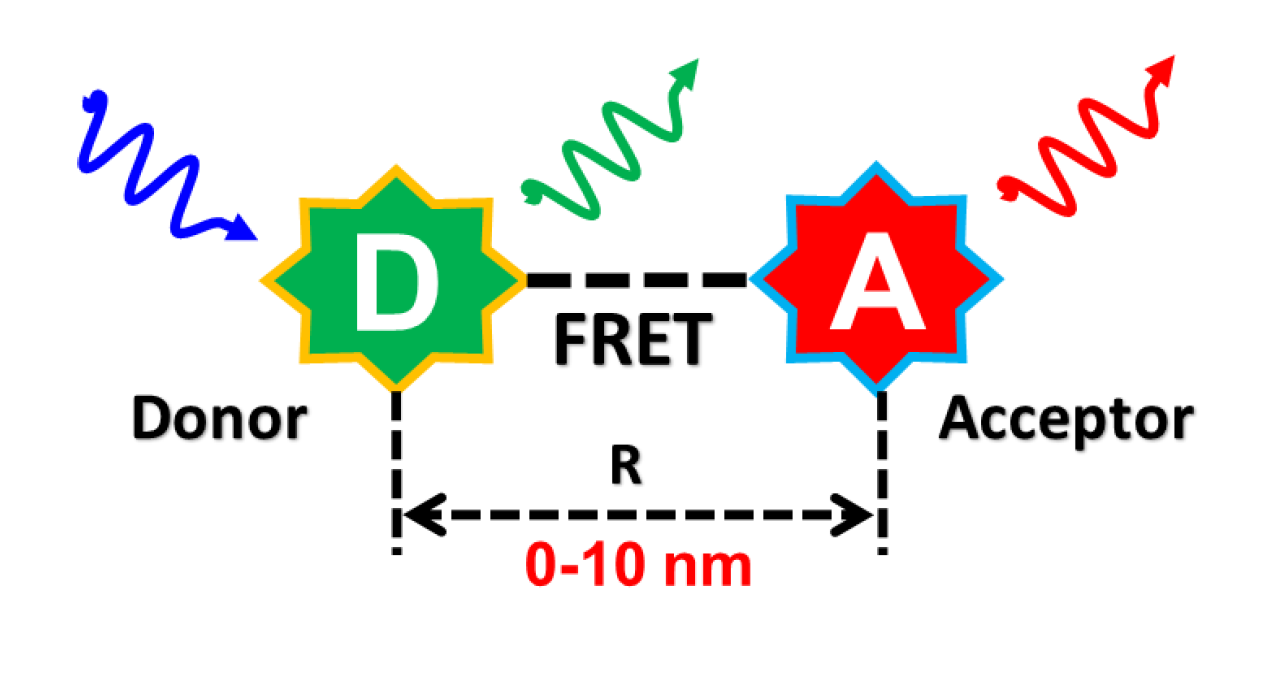
\includegraphics[width=0.5\linewidth]{../figures/1/1_FRET过程示意图.png}
    \caption{FRET过程示意图\ref{}}
    \label{fig:fret}
\end{figure}

理论和实验证明,当供受体荧光分子的距离为$r$时,它们之间的能量转移速率由下式给出\upcite{yekta1995dipole}:
\begin{equation}
    k_T(r)=\frac{1}{\tau_D}(\frac{R_0}{r})^6, \label{eq:1-1}
\end{equation}
其中$\tau_D$是供体荧光寿命,$R_0$为Förster半径,由下式表示:
\begin{equation}
    R_0^6=8.79\times{10^{-5}}(n^{-4}Q_DJ(\lambda)\kappa^2)(\text{in~} \mbox{\AA}^6),
\end{equation}
上式中,$n$表示介质的折射率,$Q_D$表示供体的量子产率,$J(\lambda)$是光谱重叠积分,$\kappa^2$是方向因子,表示供、受体偶极子的相对方向,一般在自由状态下取$\kappa^2=2/3$。FRET发生需要满足三个条件:(1)$r$的数值在$R_0$附近,约0-10nm;(2)供体的发射谱与受体的吸收谱有超过30\%的重叠;(3)供、受体偶极子方向不互相垂直。

FRET效率($E$)定义为供体转移给受体的能量与供体发射的总能量的比例,是用来衡量FRET程度的指标,其主要和分子间距和荧光团光谱的重叠度有关。光谱有部分重叠的供受体分子间距越小,能量转移就越高效。其计算式为:
\begin{equation}
    {E}=\frac{k_T(r)}{k_T(r)+\tau^{-1}_{D}},
\end{equation}
将公式\ref{eq:1-1}代入,可以看出$E$与$r$的六次方成反比的关系:
\begin{equation}
    E=\frac{R_0^6}{R_0^6+r^6}=\frac{1}{1+(r/R_0)^6}.
\end{equation}

\subsection{FRET在生物学中的应用}

FRET发生的条件是供、受体分子之间的距离$r$在0 - 10nm之间,这使得FRET技术成为一种“纳米尺”,能够有效地测量纳米级的分子间距。
FRET技术在研究生物蛋白相互作用、大分子构象变化、信号通路中的蛋白质调节机制等方面得到了广泛的应用\upcite{2020Single, wu2018translocation, shrestha2015understanding}。

FRET技术应用到各种生物研究中的重要前提是荧光蛋白的发展\upcite{chudakov2010fluorescent}。
1962 年,第一种绿色荧光蛋白(Green Fluorescent Protein, GFP)在维多利亚水母中被发现,由于荧光蛋白的无毒性以及稳定遗传性,可以利用基因转导技术将荧光蛋白接到感兴趣的蛋白质分子上,借助显微成像技术实时观察活细胞中目标蛋白的转位以及信号传递等生物问题\upcite{shimomura2009discovery}。
随着基因技术的发展,最先发现的GFP 蛋白被改造出了多种GFP突变体,多种荧光蛋白的出现为同时追踪多个蛋白质分子间的相互作用和多种蛋白质的共定位等复杂的生物问题提供了必要条件,使得基于FRET显微成像技术在分子生物学和以及生物物理学的活细胞在体研究得到了广泛的应用\upcite{sekar2003fluorescence}。

FRET定量分析方法的发展,如$3^3$-FRET(Three-cube FRET)、E-FRET(Emission FRET)和FRET双杂交分析(FRET Two-hybrid Assay)等,帮助研究人员从独特的角度研究细胞内蛋白质等大分子的相互作用\upcite{erickson2001preassociation,zal2004photobleaching}。
2016年,Ben-Johny等人利用FRET双杂交分析技术定量研究了钙离子通道与钙调蛋白之间的结合,发现当细胞内钙离子浓度较低时,一个钙调蛋白与一个钙离子通道结合;当细胞内钙离子浓度较高时,一个钙离子通道可以同时结合两个钙调蛋白\upcite{ben-johny2016}。
杨方方等人利用FRET双杂交实验,研究了Bcl-2家族的四种抗凋亡或促凋亡蛋白(即Bcl-xL、Bad、Bax和tBid)在健康细胞和凋亡细胞中的相互作用。\upcite{yang2020stoichiometry}。
李小梅等人使用双杂交FRET成像等技术对L型钙通道C末端编码肽进行了定量研究,证明了Calmudolin的多种变体均通过与钙调素竞争,抑制钙通道的基本功能\upcite{yang2022cytosolic}。

基于FRET技术在活细胞内实时监测钙离子的动态变化操作简单,灵敏度更高。
Cornea 等在2009利用荧光共振能量转移技术研究了钙调蛋白(CaM)与骨骼肌 Ryanodine 受体(RyR1)的结合模式\upcite{cornea2009fret}。
2020年Yoon等开发了一种基于 EGFP 和 Fusion Red 的新型 FRET 钙传感器(FRET-GF-PRed),并结合高频超声(HFU)技术实现了单细胞水平的精准刺激与成像\upcite{yoon2020fret}。
Yi等人开发红色电压指示剂 Cepheid1,利用 eFRET 技术实现单细胞电活动与钙信号同步监测,揭示了胰腺细胞电振荡与钙波动的时空关联\upcite{han2023bright}。

FRET还可用于检测酶的活性\upcite{carmona2009use, walter2021coumarin}。
酶支配着生物体内的新陈代谢、营养和能量转换等许多催化过程,影响着生物体内许多信号转导过程。
Cheppali等利用单分子三色 FRET 监测 NSF 酶解聚 SNARE 复合体的过程,揭示其解聚存在两条路径,澄清了酶作用的中间状态机制\upcite{cheppali2025single}。
樊林玮等通过 FRET 传感器发现机械牵张激活 cPLA2,抑制脂肪酸氧化酶活性,通过调控转录因子 YY1 影响血管平滑肌细胞功能\upcite{fan2025mechanical}。

在疾病诊断方面,FRET 技术在药物疗效评估等方面同样具有重要意义\upcite{song2011development, sun2021recent,双杂交药筛}。
2014年,Bozza等人通过设计特定的 FRET 生物传感器,能够直接反映癌症药物诱导癌细胞凋亡的效果,为药物的研发和筛选提供了有力的工具,避免了因无法区分细胞死亡和生长抑制而导致的结果偏差\upcite{bozza2014use}。

\subsection{基于受体敏化发射的FRET定量测量方法(E-FRET)}

受限于实验仪器和样本的准备,早期的FRET测量方式都只能基于定性或半定量测量\upcite{awais2004A,Aye2009Fluorescent}。
复杂实验条件的校正,需要使用表达特定荧光蛋白的细胞进行校正,而蛋白质在细胞中的表达又受到表达的成熟度、胞内的微环境等多种因素制约\upcite{liu2018influence}。

基于受体敏化发射的通道方法(E-FRET)具有测量速度快、无损伤的特性,被公认是最适合用于活细胞动态监测的FRET半定量检测技术\upcite{erickson2001preassociation}。
E-FRET方法需要对实验系统响应和荧光团的光学性质进行严格的校准,一般通过提前测量多个参照样本,然后保持在整个实验过程中系统的稳定和实验条件的一致。
E-FRET方法需要3个Cube组成的3个通道,分别实现供体激发供体收集(DD通道)、供体激发受体收集(DA通道)和受体激发受体收集(AA通道)。
受体的敏化荧光从DA通道测得($I_{DA}$图像),但实际上$I_{DA}$图像包含有供体转移到受体的敏化荧光、供体激发光直接激发受体的荧光和供体受激发的发射荧光这三个部分。
为了消除后两部分串扰,需要收集额外的DD通道和AA通道的荧光图像$I_{DD}$和 $I_{AA}$。通过减掉串扰得到敏化荧光$F_C$,由如下公式得到:
\begin{equation}
F_C=I_{DA}-a(I_{AA}-cI_{DD})-d(I_{DD}-bI_{AA}) ,
\label{eq:fc}
\end{equation}
其中$a, b, c, d$是串扰系数,由单转的供体样本和单转的受体样本得到,其计算公式如下:
\begin{align}
a&=\frac{I_{DA}(A)}{I_{AA}(A)}, \label{eq:a}\\
b&=\frac{I_{DD}(A)}{I_{AA}(A)}, \label{eq:b}\\ 
c&=\frac{I_{AA}(D)}{I_{DD}(D)}, \label{eq:c}\\ 
d&=\frac{I_{DA}(D)}{I_{DD}(D)}, \label{eq:d}
\end{align}
其中,$I_{DA}(A)$表示单转受体(A)样本在DA通道测得的荧光强度,其他参量意义类似。

E-FRET还需要测量得到荧光强度由DD通道转换为DA通道的转换因子$G$,在仪器系统参数保持不变时,$G$因子可以通过敏化发射荧光$F_C$在受体光漂白后荧光减少与受体光漂白后供体在DD通道的荧光恢复的比值确定,其定义如下:
\begin{equation}
    G=\frac{F_C-F_C^{post}}{I_{DD}^{post}-I_{DD}}, 
    \label{eq:g}
\end{equation}
其中$I_{DD}^{post}$是受体光漂白后受体敏化发射的荧光强度,$I_{DD}^{post}$是受体光漂白后供体的荧光强度。
获得敏化淬灭转化因子$G$和敏化发射荧光强度$F_C$后,供体角度的FRET效率$E_D$可以通过如下公式计算:
\begin{equation}
    E_D=\frac{F_C}{F_C+G \cdot I_{DD}}.
    \label{eq:ed}
\end{equation}
% \vspace{-2.5em} % 减少与后续文字的垂直间距

为了确定待测样本中受体与供体的浓度比例,需要首先通过测量受体与供体比例为1:1的FRET固定质粒样本来确定发生FRET时相等浓度的供体荧光和受体荧光的比例\upcite{chen2006measurement}:
\begin{equation}
    k=\frac{I_{DD}+F_C/G}{I_{AA}}.
    \label{eq:k}
\end{equation}
然后使用$k$测量待测样本中的受供体浓度比$R_C$,计算方式为:
\begin{equation}
    R_C = \frac{[A]}{[D]} = \frac{k \cdot I_{AA}}{I_{DD} + F_C/G}.
    \label{eq:rc}
\end{equation}

\section{FRET双杂交分析技术}

\subsection{基于Langmiur模型曲线拟合的FRET双杂交分析(L-FRET)}
蛋白质之间相互作用的化学计量比是阐明蛋白质间相互作用机制的重要参数,确定化学计量比能够进一步评估蛋白质间的生物相关性,并且能够确定其病理角色\upcite{zhao2020quantitative, clark2023single}。
传统的体外生化方法往往都需要从细胞中分离并且提纯大分子复合物才能进行测量,这类体外实验方法无法在活细胞中获得结果,而且一些大分子的复合物不容易进行分离提纯或者体外重建,这就限制了这些体外方法的应用\upcite{cui2019techniques}。

FRET过程改变了供受体复合物荧光发射谱的两个方面:(1)供体荧光淬灭;(2)受体荧光增强。
从这两个方面出发,FRET效率也可以从两种方式进行测量:(1)通过E-FRET方法从供体角度测量的FRET效率$E_D$,即供体转移给受体的能量占供体总能量的比例;(2)通过$3^3$-FRET方法从受体角度测量的FRET效率$E_A$,即受体敏化发射的荧光量占所有供体能量转移给受体时受体的荧光发射总量的比例。
$3^3$-FRET方法中,$E_A$可由如下公式给出:
\begin{equation}
    E_A = \frac{F_C}{a \cdot I_{AA}} \frac{\varepsilon_A}{\varepsilon_D},
    \label{eq:ea}
\end{equation}
其中,$\varepsilon_A / \varepsilon_D$是受体和供体的摩尔消光系数之比,$a$是光谱串扰系数,由公式 \ref{eq:a} 确定。

FRET双杂交分析是目前唯一可以在活细胞内进行生物大分子结合“滴定”实验的技术。
FRET双杂交分析实验中,通过不断增加受体的浓度使得每个供体都结合有受体,从而测出饱和结合时供体角度探测的最大$E_D$($E_{D,max}$)。
同样的方法,通过不断增加供体的浓度使得每个受体都结合有供体,从而测出饱和结合时受体角度探测的最大$E_A$($E_{A,max}$)。
在存在自由供体、自由受体和以$n_D:n_A$比例结合的受供体复合物($n_DD$-$n_AA$,$n_D$和$n_A$是供体和受体在复合物中的数量),当所有供体都被受体结合时,每个供体预期的能量转移效率为
\begin{equation}
    E_{D,max}=\frac{1}{n_D} \sum_{i=1}^{n_D} \sum_{j=1}^{n_A} E_{ij}.
\end{equation}
当所有受体都被供体结合时,每个受体预期的能量转移效率为
\begin{equation}
    E_{A,max}=\frac{1}{n_A} \sum_{i=1}^{n_D} \sum_{j=1}^{n_A} E_{ij}.
\end{equation}
于是,$E_{A,max}$与$E_{D,max}$的比值即为供受体的化学计量比:
\begin{equation}
    \upsilon = \frac{n_D}{n_A} = \frac{E_{A,max}}{E_{D,max}}. \label{eq:stoic}
\end{equation}

2016年,Butz等人提出将FRET效率和自由受供体浓度按照Langmiur模型进行拟合的FRET双杂交分析方法\upcite{butz2016}。
对于包含自由供体、自由受体和供受体复合物中,$E_D$和$E_A$可分别与自由受体浓度、自由供体浓度相关联:
\begin{align}
    E_A = E_{A,max} \frac{D_{free}}{D_{free}+K_{d,EFF}}, \label{eq:eadfree} \\
    E_D = E_{D,max} \frac{A_{free}}{A_{free}+K_{d,EFF}}, \label{eq:edafree}
\end{align}
其中,$K_{d,EFF}$为相对解离常数,$D_{free}$是自由供体的浓度,$A_{free}$是自由受体的浓度。
从公式 \ref{eq:eadfree} 和公式 \ref{eq:edafree} 可以看出,与体外滴定实验类似,用$3^3$-FRET法可得到$E_A$随自由供体浓度变化的动态滴定曲线,并得到$E_{A,max}$,用E-FRET方法也可以得到$E_D$随自由受体浓度的动态滴定曲线,并得到$E_{D,max}$。供受体复合物的化学计量比计算与公式 \ref{eq:stoic} 相同。

\subsection{\texorpdfstring{基于FRET效率$E_D$和受供体浓度比$R_C$线性分离的FRET双杂交分析}{基于FRET效率Ed和受供体浓度比Rc线性分离的FRET双杂交分析(DC-FRET)}}

L-FRET方法存在一定的局限性。从实验条件上来看,L-FRET需要得到FRET效率与自由供体/自由受体间的饱和滴定曲线,这意味着实验人员需要精心准备不同供受体浓度比的样本,并且这些样本的供受体浓度分布要尽可能均匀。
因此L-FRET往往需要配备一系列梯度比例的供体和受体溶液,然后分别对其进行混合和检测,这增加了实验样本的数量。
在实验数据处理时,大量浓度梯度都需要进行测量和数据处理,这极大地增加了实验人员的工作量和操作难度。
另一方面,从公式 \ref{eq:eadfree} 和 \ref{eq:edafree} 来看,$A_{free}$和$D_{free}$是拟合过程中更新的中间量,在实际的计算分析过程中,由于这些中间量的不确定性以及数据的复杂性,很容易出现拟合失败的情况。
一旦拟合失败,就需要重新进行实验或者调整参数,进一步增加了实验成本。

为了解决这些问题,在2018年,Du等人创新性地发展了基于FRET效率($E_D$)和受供体浓度比($R_C$)线性分离的FRET双杂交分析方法,简称为 Du-Chen-FRET(DC-FRET)\upcite{Du2018}。
DC-FRET聚焦关注分析供体饱和结合和受体饱和结合的数据。
当供体完全饱和时,即$D_{free}>>K_d$,此时受体被完全结合,以下公式成立:
\begin{align} 
    E_A &= E_{A,max}, \label{eq:ea_appro} \\
    E_D &= {E_{A,max}}{\cdot}{R_C}. \label{eq:ea_slope}
\end{align}
此时$E_D$与$R_C$成正比,且斜率为$E_{A,max}$。
当受体饱和时,即$A_{free}>>K_d$,此时供体被完全结合,以下公式成立:
\begin{align}
    E_D &= E_{D,max}, \label{eq:ed_appro} \\
    E_A &= E_{D,max}{\cdot}{1/R_C}. \label{eq:ed_slope}
\end{align}
此时$E_D$与$R_C$成正比,且斜率为$E_{A,max}$。
求得$E_{A,max}$和$E_{A,max}$后,供受体复合物中的化学计量比计算同公式 \ref{eq:stoic} 。

DC-FRET方法相比L-FRET方法有着一定的优势。
首先,在实验准备阶段,L-FRET由于需要得到FRET效率与自由供体/自由受体间的饱和滴定曲线,因此需要准备大量不同浓度的供体和受体样本,才能保证滴定曲线拟合的准确性。
DC-FRET方法只需要准备$R_C$比较大的样本和$R_C$比较小的样本,省去了不饱和结合的样本准备工作。
其次,L-FRET方法因为采用参数迭代拟合计算,容易放大异常数据带来的影响,从而出现结果超出物理意义范围或者出现不合理的结果,鲁棒性较差;DC-FRET方法线性拟合需要的$E_A$、$E_D$和$R_C$数据是$3^3$-FRET和E-FRET方法直接测量得到的,其数据可靠且方便筛选,通过这种方式得到的数据进行线性拟合,其结果也更加稳定可靠。

\section{FRET分析数据处理方法现状}

\subsection{FRET双杂交分析数据处理现状}
FRET 双杂交数据处理流程复杂耗时,人工依赖程度高,严重制约了实验效率与数据可重复性。
Butz 等指出,数据处理包括图像分析、FRET 定量计算及双杂交分析等多个环节,共28个步骤,单次实验数据处理过程需要 3.5 - 7 小时不等\upcite{butz2016}。
在图像分析环节,科研人员需手动标注上百个典型荧光区域作为 ROI,逐一定量灰度值并计算荧光信号与背景值,这一过程通常耗时 1 - 3 小时。
在 FRET 定量计算阶段,研究人员需将标注三通道荧光强度数据,再通过 Excel 设定公式完成批量计算,包括敏化发射荧光和 FRET 效率等参数。
这一过程虽部分实现自动化,但仍需人工输入数据并验证公式逻辑,耗时约 30 分钟至 1 小时。
在双杂交拟合计算中,使用 Excel 规划求解拟合 Langmuir 模型需经历 14 个步骤,耗时约 30 分钟。

通用软件缺乏针对 FRET 双杂交的优化。
Zen和ImageJ等通用软件可以手动标注ROI,但是缺少直观的辅助信息如信号背景比等,更无法展示FRET效率等直观的结果。
Excel 的规划求解功能在处理非线性拟合时灵活性不足,常需结合编程工具进行二次开发,频繁在 Excel 与 Matlab / Python 等工具间转移数据。

传统数据处理流程对科研人员的技术要求较高,不利于实验结果的复现和对比。
FRET图像处理中,人工标记 ROI 是一种盲处理,要求实验人员拥有丰富的处理经验和专业知识。
此类人工操作不仅效率低下,还因缺乏操作规范,易引入主观偏差,影响数据的可复现性。
在面对动态荧光事件或低信噪比数据时,人工分析的主观性与低效性尤为突出\upcite{zhou2024deep}。

这些挑战促使科研人员探索更高效的自动化解决方案,以推动 FRET 技术在生物医学研究中的广泛应用。

\subsection{基于机器学习的FRET数据处理}
近年来,随着机器学习不断发展,越来越多的研究者着手将此类方法应用于 FRET 数据分析。

深度学习技术为单分子FRET技术中高效解析动态轨迹数据提供了新方法。
Li等基于长短期记忆(Long Short-Term Momery, LSTM)和卷积神经网络(Convolutional Neural Network, CNN)的 AutoSiM 框架,自动分类和分割单分子荧光轨迹,提升 SiMREPS 检测灵敏度与 smFRET 分析效率,支持迁移学习适应新数据\upcite{li2020automatic}。
Zhang等人提出基于LSTM的Kin-SiM框架通过预训练模拟数据自动识别 smFRET 轨迹中的分子状态及动力学参数,实现轨迹理想化,性能与传统 HMM 相当但效率更高,支持多任务学习适应不同状态数\upcite{zhang2025pretrained}。
Miao等提出基于深度学习的局部特征分类框架DEBRIS和多帧双通道融合去噪网络(MUFFLE),通过滑动窗口技术和用户自定义标准,自动识别双色/单色单分子荧光事件。

多分子FRET技术中,应用深度学习技术可以提高选取FRET荧光信号的效率,避免了重复的人工数据处理。
Ge等人研发出一种基于 U-Net 模型的深度学习方法进行高效FRET分析,该模型基于一个包含230个手动标注ROI的数据集进行训练,随后通过旋转操作将数据集扩充,最终得到 2760 个样本\upcite{ge2020}。
U-Net 模型是图像分割领域广泛运用的卷积神经网络架构,它能够有效捕捉荧光图像的特征,精准地分割并提取 ROI 的荧光强度信息\upcite{ronneberger2015u}。
Thomsen 等人开发的 DeepFRET 软件基于深度学习技术,实现了从原始显微镜图像到 FRET 数据分类的全自动化流程\upcite{thomsen2020deepfret} 。
该软件通过预训练的深度神经网络对荧光轨迹进行逐帧分类,仅需用户设定质量阈值,即可快速生成高质量的 FRET 直方图。
Feldmann 等在进行FRET双杂交分析数据处理时采用了ilastik这一用于生物医学图像分析的开源交互式工具,将机器学习算法与用户交互相结合,能减轻手动标注的工作量\upcite{feldmann2023, berg2019ilastik}。

然而,机器学习驱动的FRET图像分析算法仍存在一定局限性。
首先,模型训练和泛化的效果依赖优质的数据集,而FRET图像的手动标注需专业知识且耗时费力,导致优质数据稀缺\upcite{kromp2020annotated}。
其次,深度人工神经网络模型的训练需要高性能图形处理器,伴随较长的训练时间,数据集越大,训练占用的时间可能会越久\upcite{9120226, huang2018gpipe}。
此外,深度学习模型的 “黑箱” 特性使其缺乏可解释性\upcite{zhang2021survey, fan2021interpretability}。
就基于强度的 FRET 定量分析而言,神经网络虽然能够捕捉图像的细微特征,但却无法用清晰的数学框架来解释决策逻辑,而且可能会引入未知的偏差。

\section{本文的工作内容和意义}

针对活细胞 FRET 双杂交分析数据处理存在的数据孤岛、流程繁琐、强人工依赖等核心问题,本文从以下方面开展了工作:

(1)首次设计并实现了针对FRET双杂交分析技术的数据处理软件 Fretha。
基于FRET双杂交分析技术的数据特点和处理流程,本文划分了成像参数设置、数据校验、FRET图像处理、数据管理、结果可视化等功能模块,并设计了用户友好的操作界面。
基于分层架构构建,Fretha由底层向上分为数据层、数据接口层、业务层和表现层。
通过封装 FRET 计算器、图像处理器和双杂交求解器,Fretha实现了E-FRET、$3^3$-FRET、DC-FRET、L-FRET等多种算法,为FRET定量分析计算提供了后台计算的能力。
软件采用 Qt 5.15.2 开发,支持跨平台部署,并通过 OpenCV 和 Dlib 库实现图像处理与优化计算\upcite{陆文周2015Qt5, bradski2000opencv, bradski2008learning}。
Fretha实现了从原始图像到化学计量比结果的一键式分析,有效替换了5款专业软件,避免了软件工具的切换,使得数据处理更加简单高效。
Fretha的推出,将有效降低FRET双杂交分析技术的使用门槛,提高实验结果的可对比性和可重复性,推动FRET双杂交技术在生物大分子相互作用研究中的应用。

(2)对 Fretha 软件进行了系统的验证和测试。
本文通过对标准质粒进行$3^3$-FRET和E-FRET分析,测得C4Y、C10Y、C40Y和C80Y的$E_A$、$E_D$和$R_C$值,测量得到的$E_{A}$值分别为$0.291\pm0.020$、$0.243\pm0.031$、$0.159\pm0.018$和$0.118\pm0.019$,$E_{D}$值分别为$0.307\pm0.040$、$0.230\pm0.022$、$0.155\pm0.011$和$0.117\pm0.012$,与文献值的相对误差分别为3.9\%、2.2\%,验证了Fretha计算FRET效率的准确性。
在FRET双杂交验证实验中,本文测量得Cerulean和Venus在C32V中的结合化学计量比为1.071,在CVC中为2.023,接近文献报道的结果,进一步验证了Fretha双杂交计算确定化学计量比的准确性。
本文针对每个功能模块单独进行了测试,以确认每个模块的功能效果,保证了软件运行时符合设计预期。
可靠性测试显示,软件在 48 小时连续运行和高频操作下保持稳定,资源占用无显著波动。
综合测试结果表明,Fretha 软件在数据处理准确性和可靠性方面均达到预期,支持连续稳定的数据处理。

(3)首次提出了基于明度和均匀度的自动ROI选取(Luminance-Uniformity-based ROI Selection, LURS)算法,实现了自动FRET双杂交分析。
LURS算法通过多通道自适应阈值分割、变异系数均匀性评估和连通区域分析,实现了荧光图像中高信噪比区域的精准识别,显著减少了人工标注 ROI 的时间成本。
结合LURS算法和鲁棒性较好的 DC-FRET 方法,Fretha软件提供了FRET 双杂交分析的数据处理全自动化,提高了大规模数据处理能力。
通过对比深度学习的方法,本文验证了LURS自动处理在性能上优于ilastik和SAM-Med2D,更适用于大数据量场景。
基于LURS算法的自动FRET双杂交分析为高通量药物筛选等大规模数据处理需求提供了高效可靠的算法工具,进一步推动了FRET双杂交分析技术的应用。

\section{本文的章节安排}
第一章,绪论。本章简要概述了定量FRET技术和FRET双杂交分析技术的理论基础和发展,然后介绍了FRET数据分析处理方法的研究现状。同时介绍了本文的工作内容和结构安排。

第二章,FRET双杂交分析数据处理软件的设计和开发。
本章基于FRET双杂交分析数据处理流程和FRET 多模态显微成像系统的特点进行需求分析,然后设计了Fretha软件的总体架构和模块划分,并详细介绍了各个模块的开发实现。

第三章,Fretha的验证和测试。
本章验证了使用Fretha进行$3^3$-FRET和E-FRET分析测量结果的准确性和稳定性,以及进行FRET双杂交分析数据处理的准确性。
针对每个模块,本章进行了单独的功能测试和性能测试,验证了Fretha软件的功能和性能符合预期。
最后,本章实施了Fretha稳定性测试,以测试Fretha长时间运行和高频操作下的稳定性。

第四章,基于LURS的自动FRET双杂交分析。
本章分析了FRET双杂交分析时的痛点,提出了基于明度和均匀度的自动ROI选择算法,并结合DC-FRET方法实现了全自动的FRET双杂交分析数据处理算法,在标准质粒和模型质粒上进行了验证实验。然后,本文还应用自动化数据处理算法分析了加药处理前后的Bcl-xL-Bak在活细胞内的相互作用,对比了深度学习方法的计算性能指标。

第五章,总结与展望。
本章总结了本文的工作内容和在相关领域的意义,对后续研究内容和方法进行展望。 


\chapter{Fretha的设计和开发}

\section{引言}
传统的 FRET 双杂交分析数据处理过程繁琐,不同处理阶段需要使用各种数据处理软件,在频繁转移数据的同时,还带来了更高的使用门槛。
开发专门针对 FRET 双杂交分析数据处理的配套软件,能够实现数据的采集、标准化处理以及高效的分析统计,对于提升实验规范性具有重要意义。

本章节介绍了FRET双杂交分析数据处理软件 Fretha 的设计和开发过程。
首先,根据课题组自研的 FRET 显微成像系统(FRETScope)的数据特征和 FRET 双杂交分析数据处理功能进行需求分析,确定了主要的数据处理流程。
对应数据处理的阶段和流程,软件被划分了相应的功能模块,减少了功能的耦合。
其次,对软件进行了分层架构设计,预留好了对应的接口,方便了软件的后续开发和扩展。
然后,基于Dlib和OpenCV等,设计了FRET定量计算器、FRET图像处理器和FRET双杂交求解器等后台接口,封装了E-FRET、$3^3$-FRET、L-FRET和DC-FRET等多模态分析算法,完成核心计算功能的实现。
最后,结合功能需求、业务逻辑、后台结构接口,完成了对各个功能模块的实现和开发。

\section{需求分析和总体设计}

\subsection{需求分析}

\ifshowtext
FRETScope是本课题组自研的适用于$3^3$-FRET、E-FRET、Pb-FRET(Photobleaching-FRET)等多种定量FRET分析方法的FRET多模态显微成像系统。
该系统具备高分辨率成像、多通道同步采集等先进特性,能够获取高质量的 FRET 三通道图像数据。
\begin{figure}[hbtp]
  \centering
  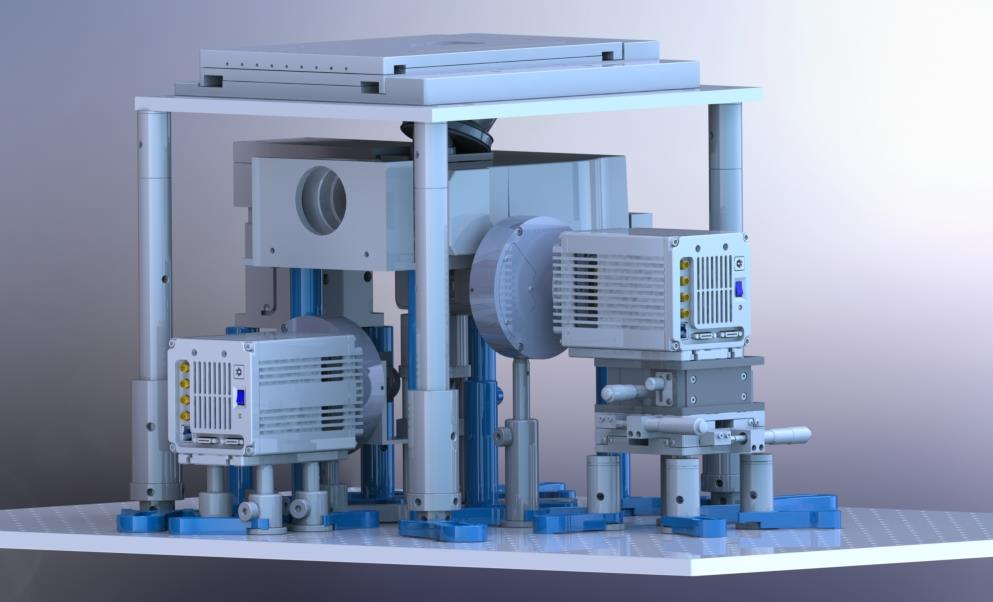
\includegraphics[width=0.9\linewidth]{../figures/2/2_FRETScope2示意图.jpg}
  \caption{FRETScope硬件外观示意图}
  \label{fig:fretscope2硬件示意图}
\end{figure}

使用FRETScope对制备好的样本进行图像采集得到若干视野的FRET三通道图像后,通过FRET双杂交分析方法定量计算细胞中的生物大分子结合作用的FRET饱和效率、化学计量比、相对亲和力等信息。FRET双杂交分析的数据处理需要如下步骤:首先需要对FRET数据进行数据完整性校验,确保每个视野下存在完整的三通道图像和文件完整可读,然后对每个视野进行荧光信号提取,通过在图像上绘制ROI并计算其灰度均值作为FRET分析计算重要的荧光信号;根据E-FRET和$3^3$-FRET方法将上述荧光信号代入对应的计算公式 \ref{eq:ed}、\ref{eq:rc} 和 \ref{eq:ea} 求取$E_A$、$E_D$、$R_C$等FRET数据;对这些数据进一步依据物理含义或者数据分析进行异常值去除等数据预处理;最后是通过优化算法拟合Langmiur模型或者线性模型计算相关的参数。具体流程如图 \ref{fig:tha_data_process} 所示。

\begin{figure}[hbtp]
    \centering
    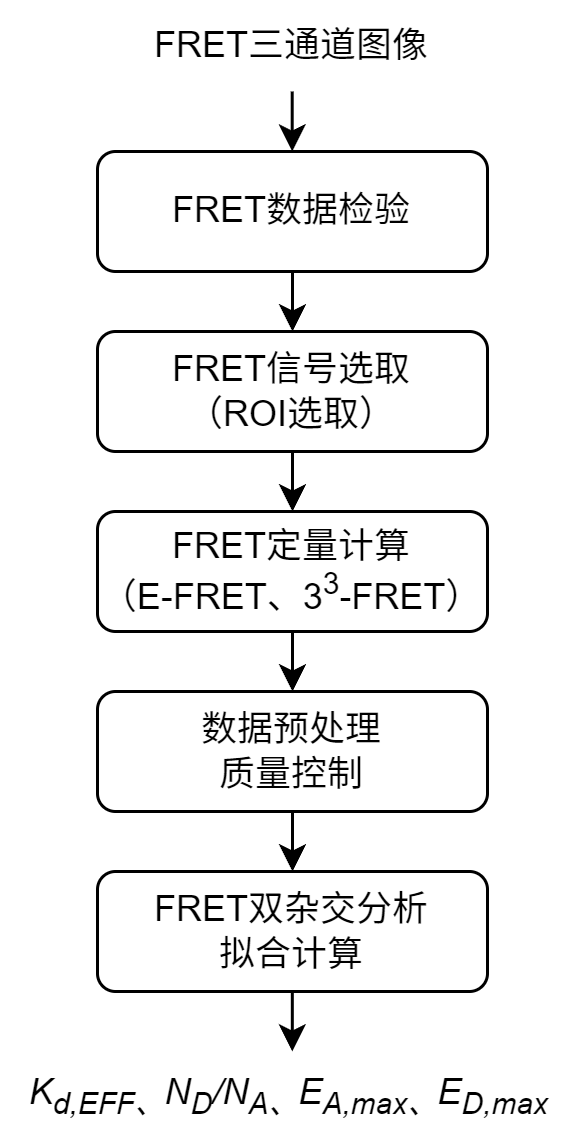
\includegraphics[width=0.4\linewidth]{../figures/2/2_FRET双杂交分析数据处理流程.png}
    \caption{FRET双杂交分析数据处理流程}
    \label{fig:tha_data_process}
\end{figure}

\fi

\subsection{模块划分和界面设计}

结合 FRET 双杂交分析的数据处理流程与功能逻辑,Fretha 软件主要划分为以下核心模块:
\begin{enumerate}
  \item {成像参数设置模块:}
  负责设置 FRET 成像过程中的成像参数,在不同实验数据处理前,需要更新对应地参数。
  该模块允许用户输入和保存成像参数,如曝光时间、串扰系数和校正因子等,并提供参数校验功能,确保参数在合理范围内,避免因参数设置错误导致数据分析处理异常。
  此外,该模块还支持将参数持久化到本地,以供多次处理数据时使用。
  \item {数据检验模块:}
  对输入数据进行命名规范和完整性等合法性检验,防止用户输入异常数据导致软件错误。
  该模块按照FRETScope系统的数据结构特征,检查每个子视野的三通道图像文件是否完整,并对文件格式和内容进行验证,确保数据的可靠性。
  \item {FRET 图像处理模块:}
  支持手动图像处理和 ROI 选取,满足用户对数据的精细化处理需求。
  手动选取感兴趣区域ROI是一个基础且关键的操作,它能帮助分析人员聚焦于细胞中荧光质量较高的区域,进行更精确的数据处理与分析。
  用户可以选择启用图像增强功能,比如归一化增强视图、生成FRET效率伪彩图等,从而提高ROI标注时的参考信息。
  该模块还提供ROI状态栏,实时计算ROI的荧光信号、视野背景、敏化发射荧光和E-FRET计算结果等,可以为ROI的质量判定提供参考。
  \item {数据管理模块:}
  数据处理模块用于增删数据、筛选数据、导入导出、开始计算等功能,还可以数据项反向定位追踪FRET图像中的ROI详情,以便检查数据和再处理。
  该模块作为FRET图像处理模块和结果可视化模块的桥梁,负责数据的统一管理和高效传递。
  \item {结果可视化模块:}
  将分析结果以直观的图表形式展示,并提供数据保存功能,方便用户进一步分析和应用。
  用户可以根据需要选择L-FRET或者DC-FRET方法的对应视图,以切换FRET双杂交分析方法。
  该模块通过在同一坐标系下绘制趋势线图和散点图,用户可以更直观地评估FRET双杂交分析计算拟合程度等。
  结果可视化模块还可以将分析结果保存为图片或数据文件,方便用户进行后续数据处理和报告撰写。
  
\end{enumerate}

在界面设计上,根据软件使用需求和模块功能,主要分为:开始页、参数设置页、数据处理页、结果页。
在软件开始页提供了跳转参数设置页或数据处理页的按钮,如图 \ref{fig:开始页界面} 所示;
\begin{figure}[hbtp]
  \centering
  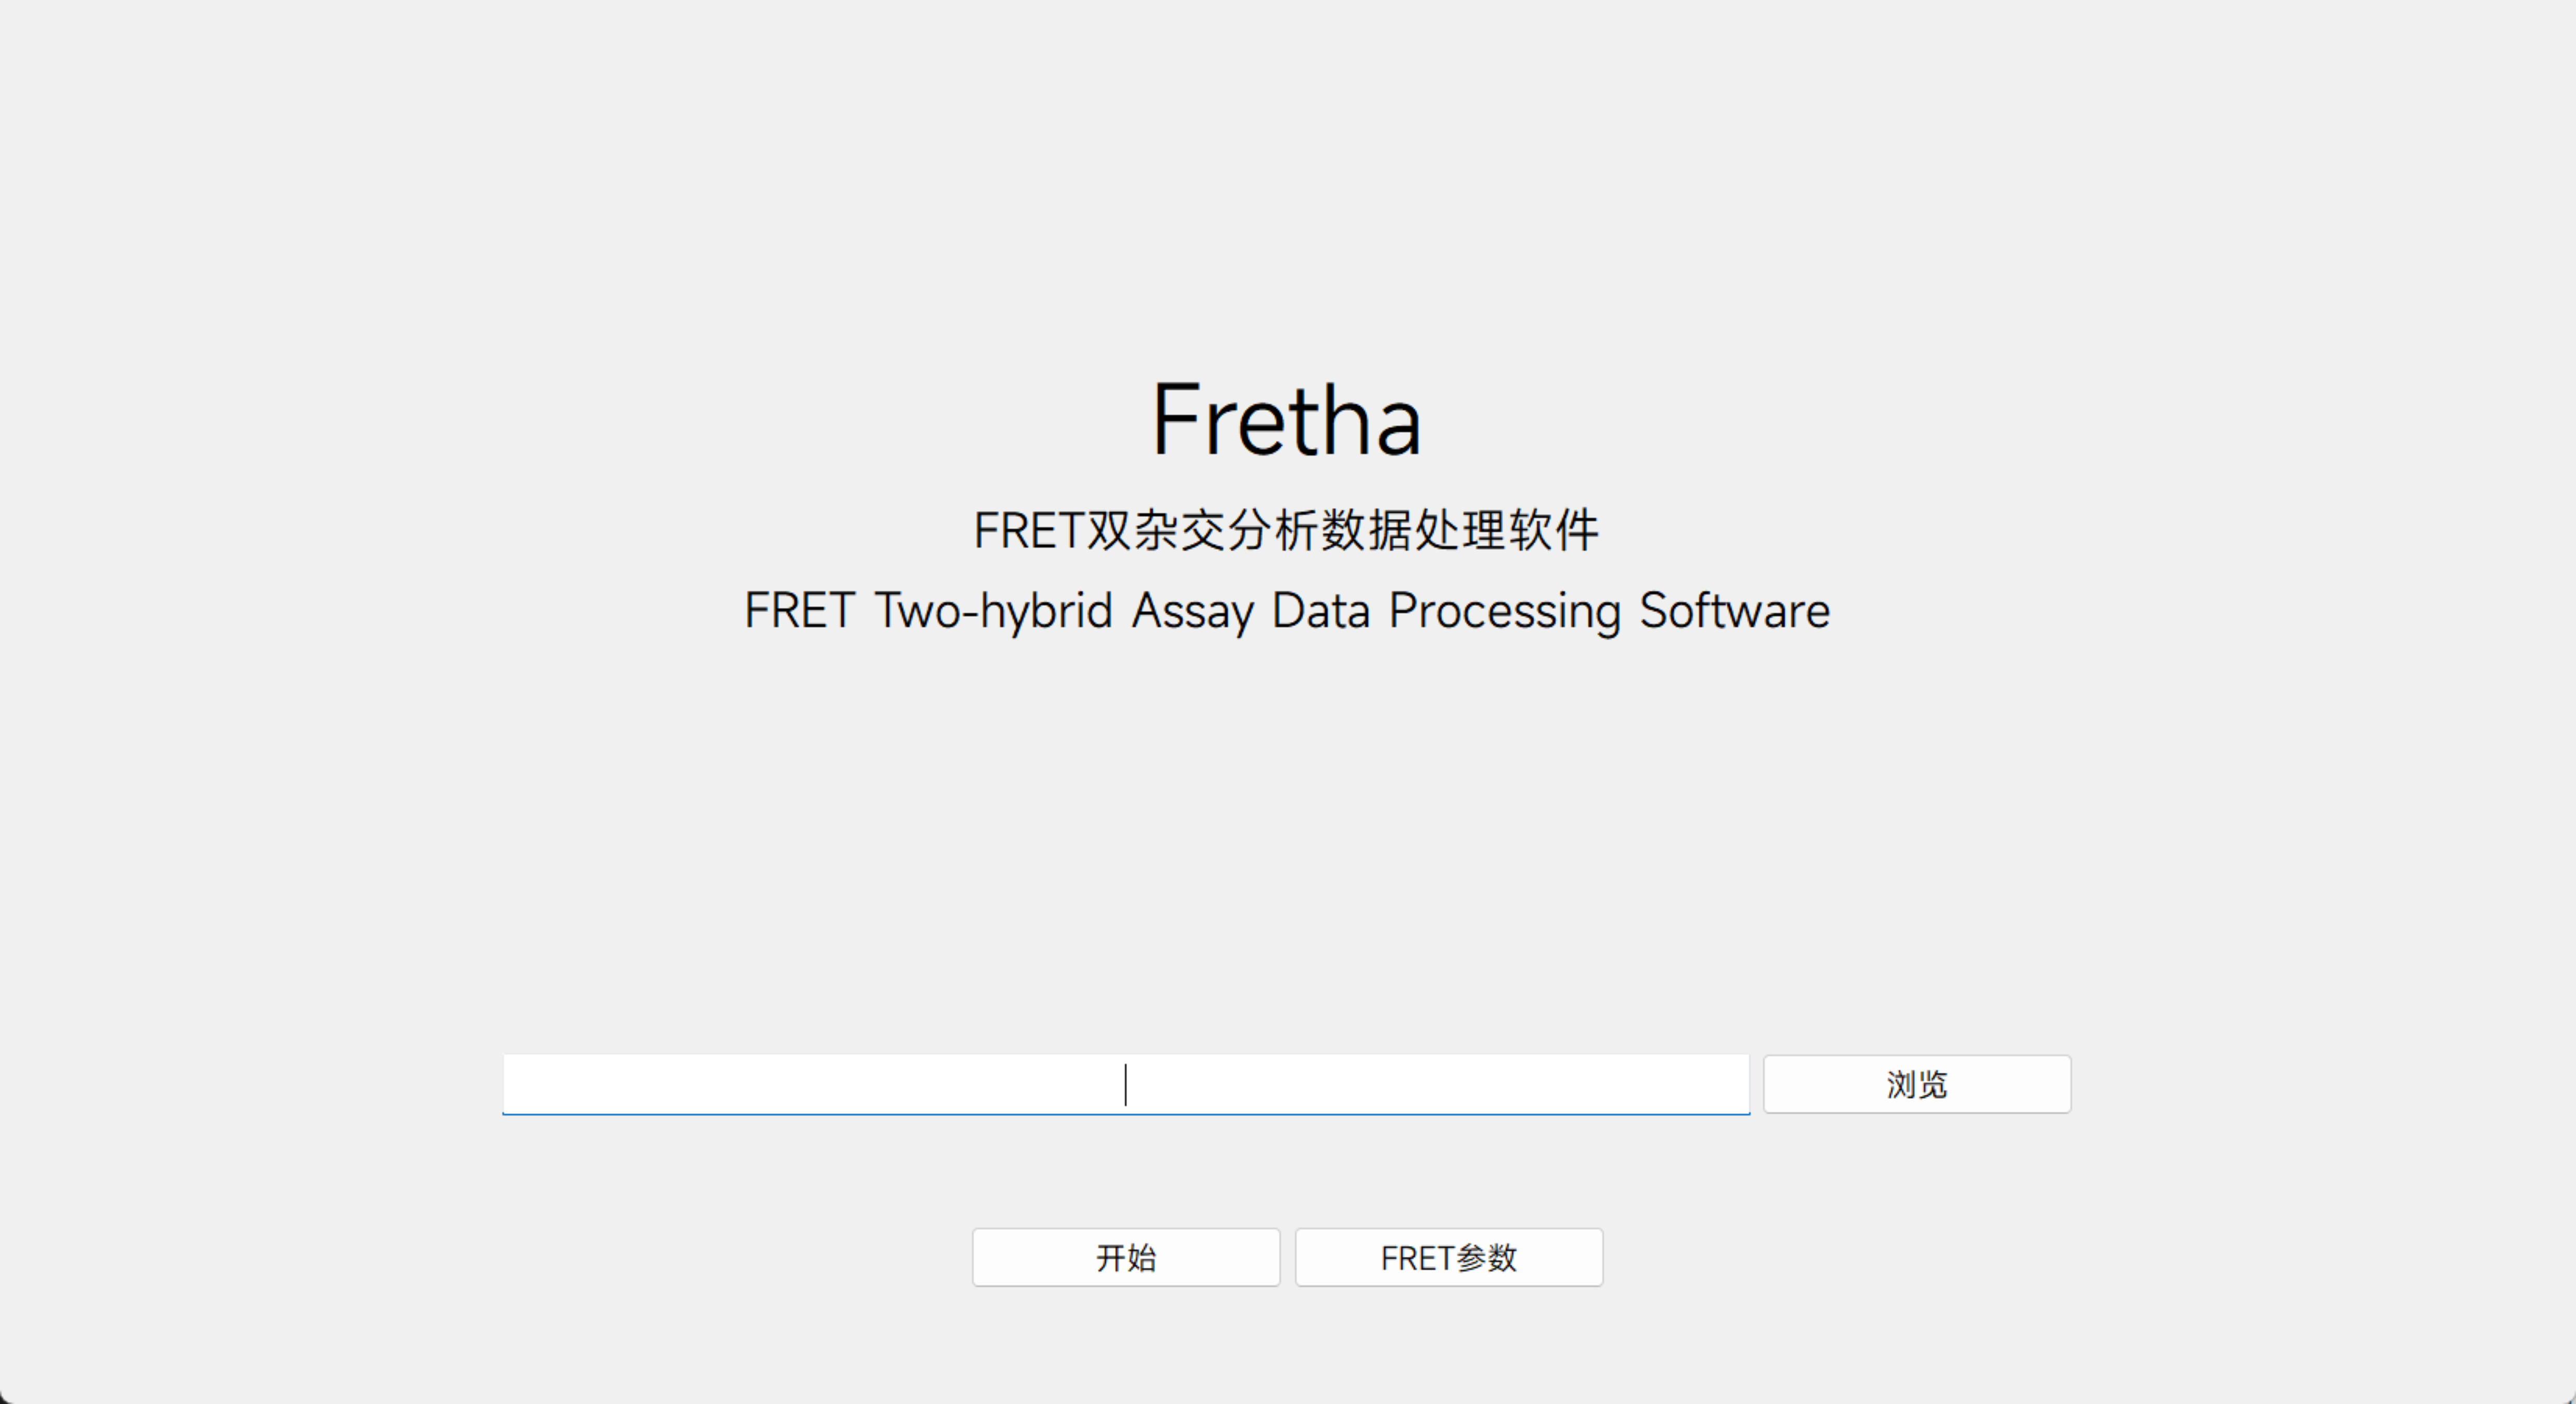
\includegraphics[width=0.9\linewidth]{../figures/2/2_开始页界面.png}
  \caption{Fretha开始页界面}
  \label{fig:开始页界面}
\end{figure}
参数设置页面包括成像参数设置模块,其界面如图 \ref{fig:参数设置页界面} 所示;
\begin{figure}[hbtp]
  \centering
  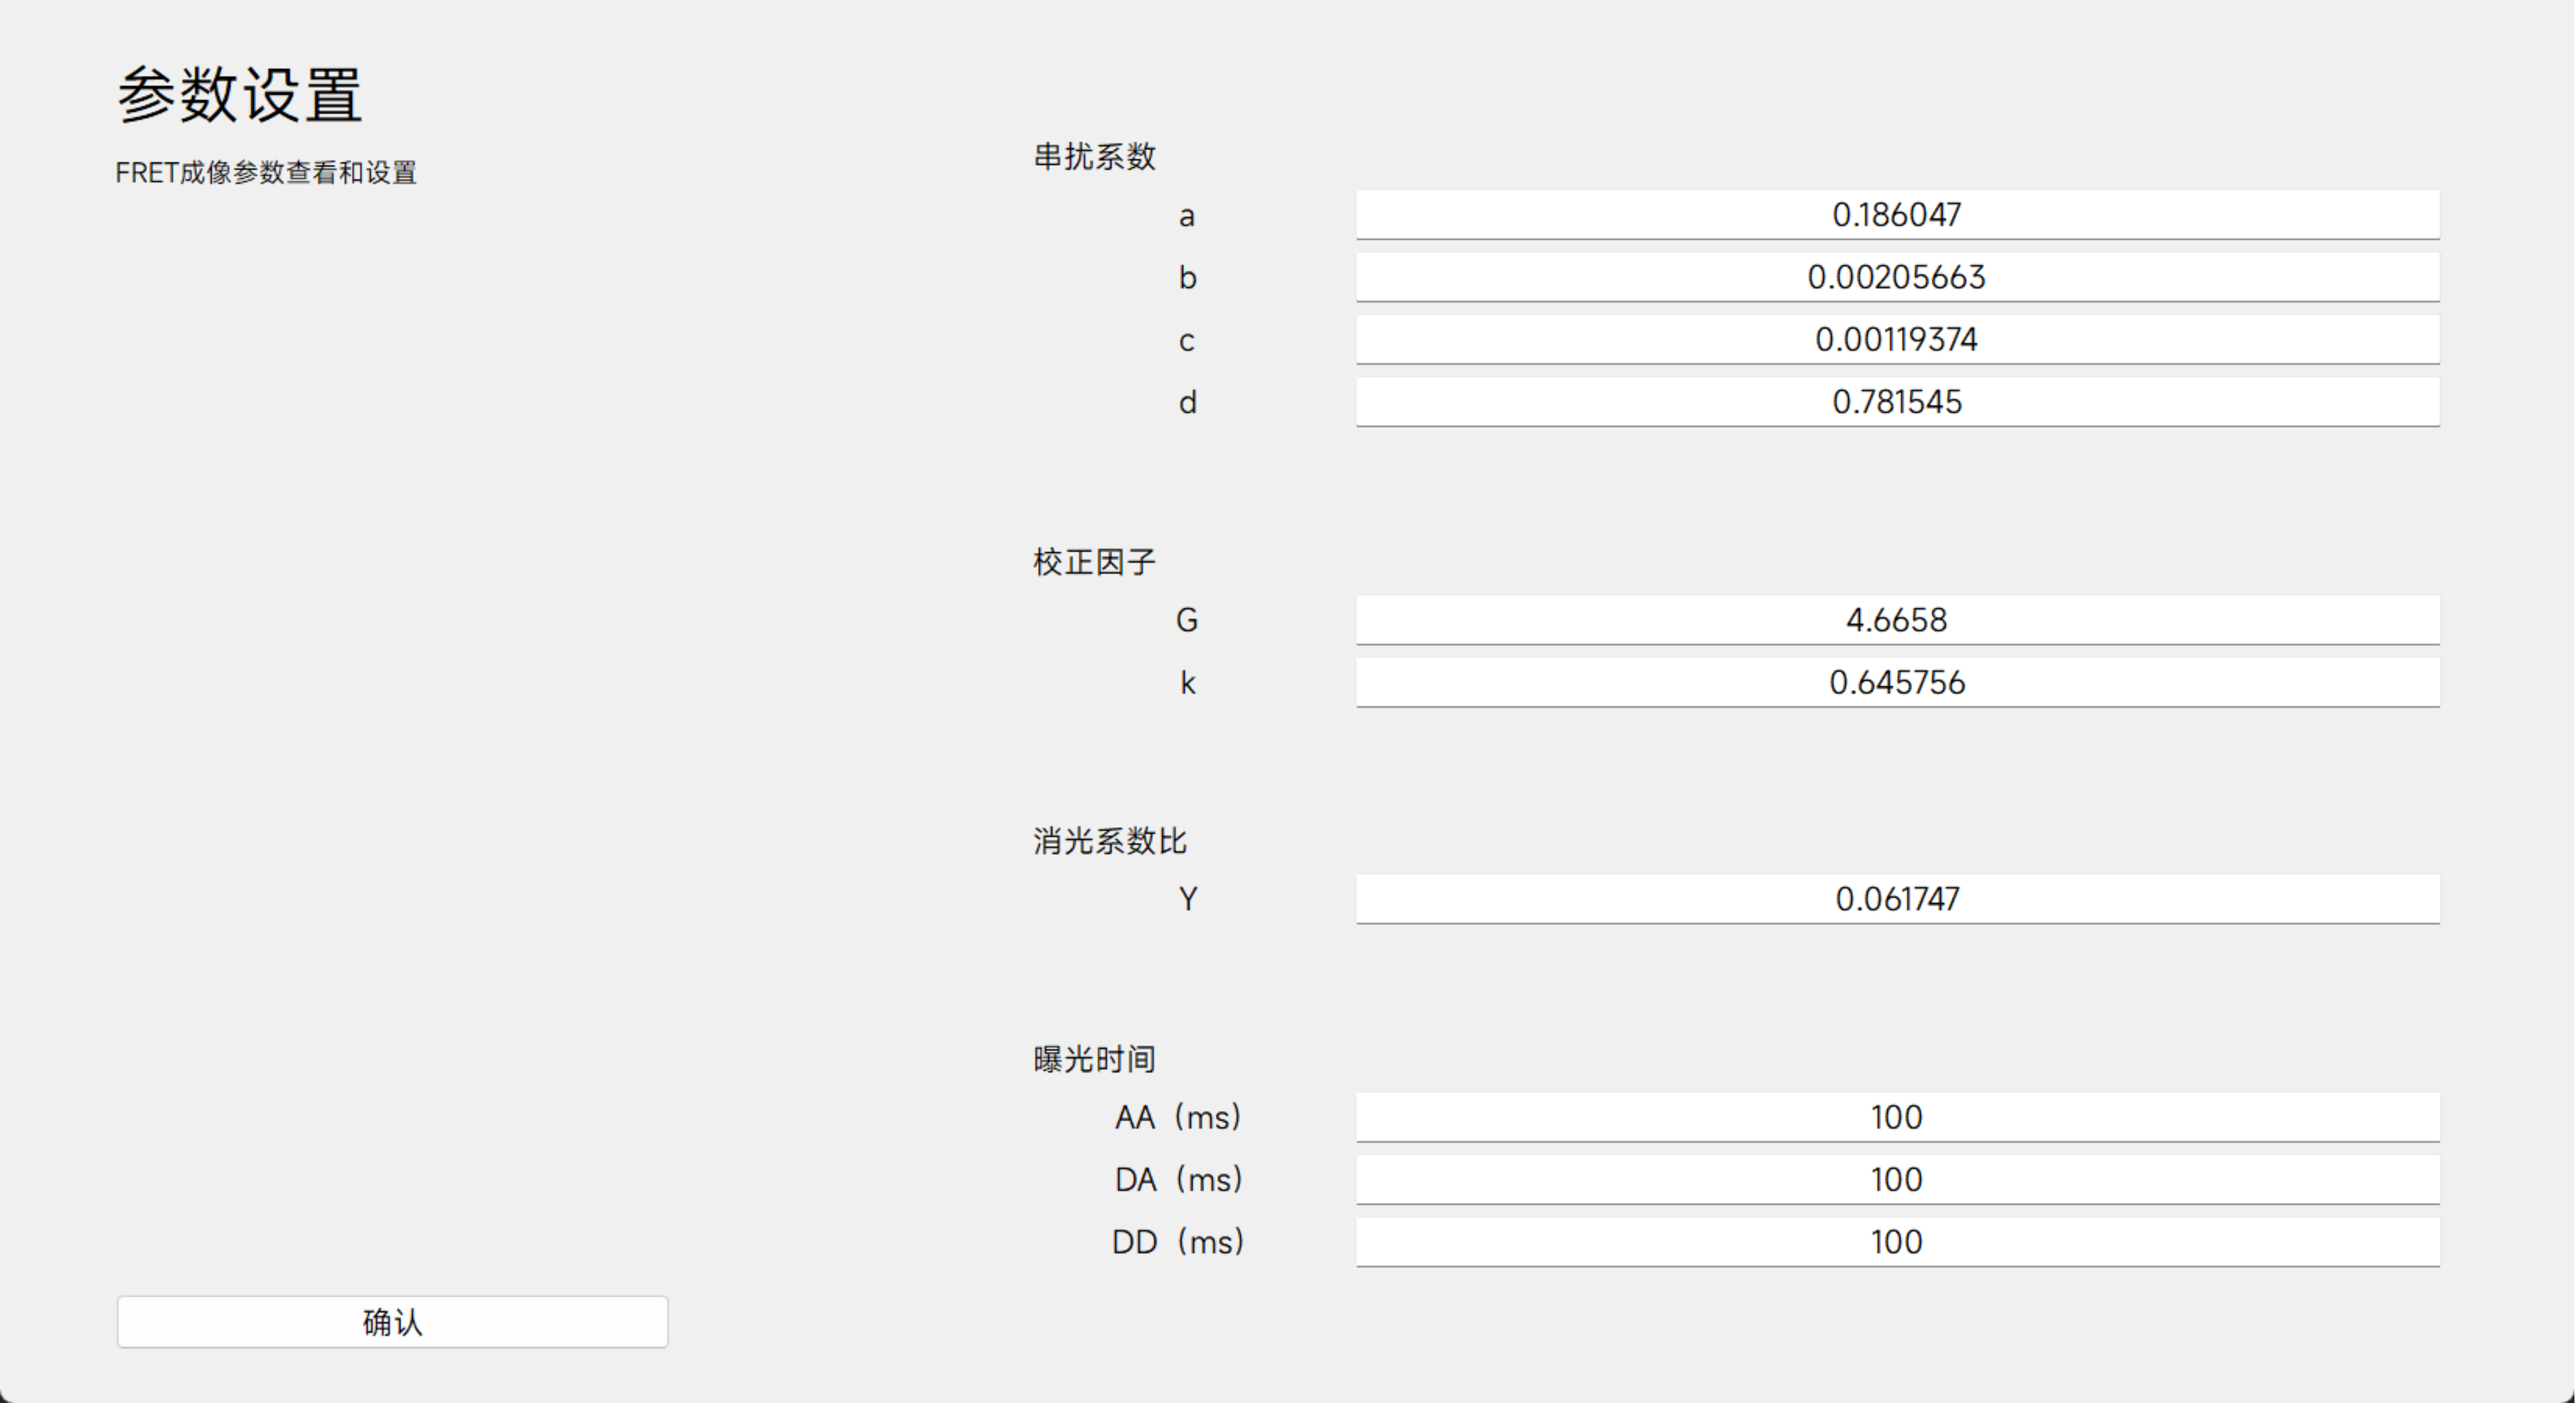
\includegraphics[width=0.9\linewidth]{../figures/2/2_参数设置界面.png}
  \caption{Fretha参数设置页界面}
  \label{fig:参数设置页界面}
\end{figure}
数据处理页包括数据检验模块的检验结果、FRET图像处理模块、数据管理模块,其界面和模块划分如图 \ref {fig:界面模块分布图} 所示;
\begin{figure}[hbtp]
  \centering
  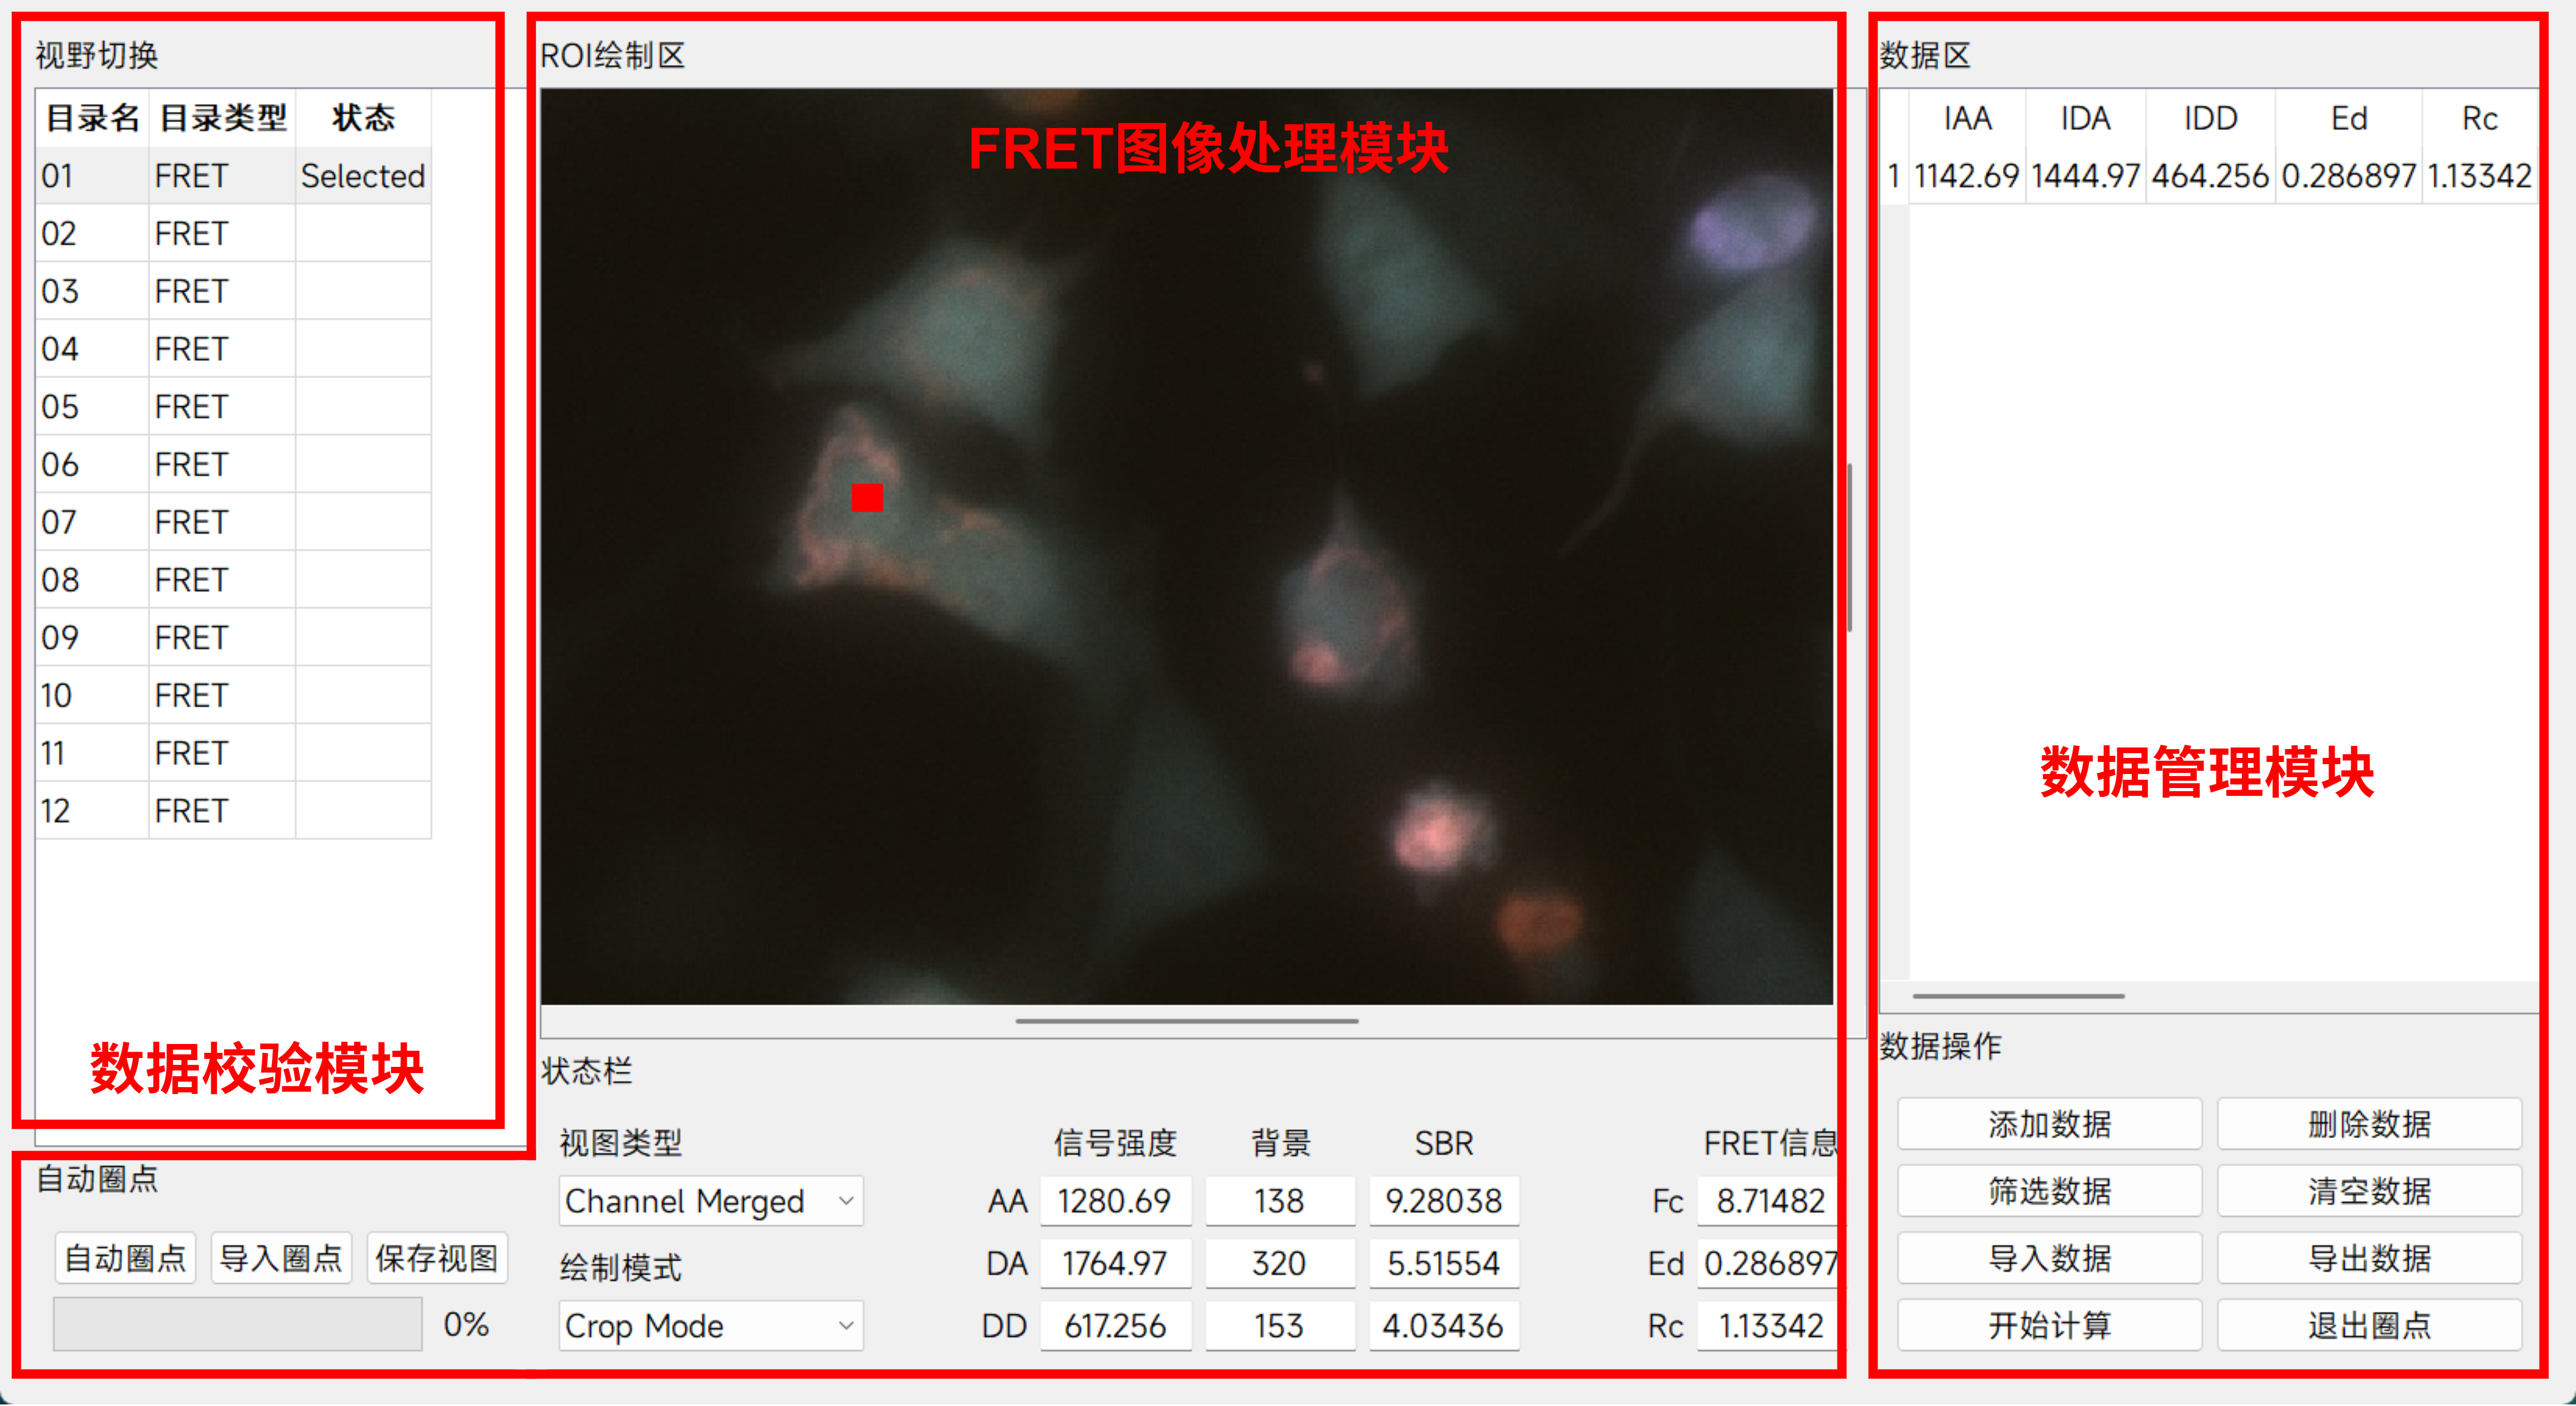
\includegraphics[width=0.9\linewidth]{../figures/2/2_模块界面.png}
  \caption{Fretha数据处理页界面及模块划分}
  \label{fig:界面模块分布图}
\end{figure}
结果页展示结果可视化模块中FRET双杂交数据处理的图像视图结果,界面如图 \ref{fig:Fretha结果可视化模块界面} 所示。
\begin{figure}[hbtp]
  \centering
  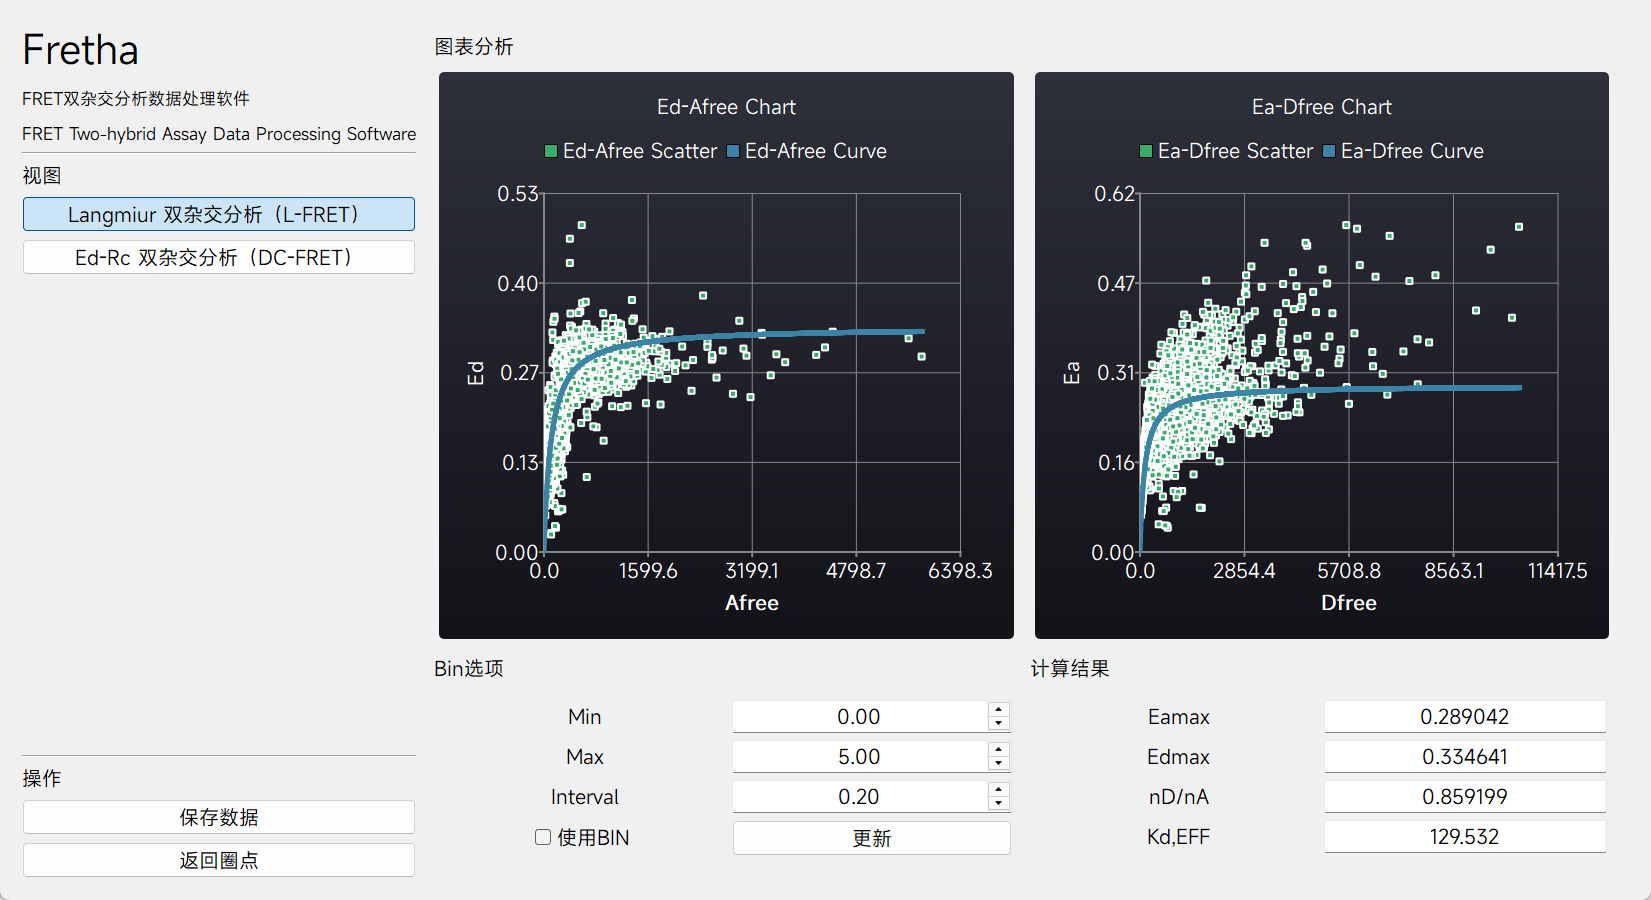
\includegraphics[width=0.9\linewidth]{../figures/2/2_结果可视化.png}
  \caption{Fretha结果可视化模块界面}
  \label{fig:Fretha结果可视化模块界面}
\end{figure}

\subsection{软件总体框架}

Fretha架构采用分层设计,由顶层向下依次分别为:表现层、业务层、数据访问层和数据层,如图 \ref{fig:fretha_arch} 所示。

\begin{figure}[hbtp]
    \centering
    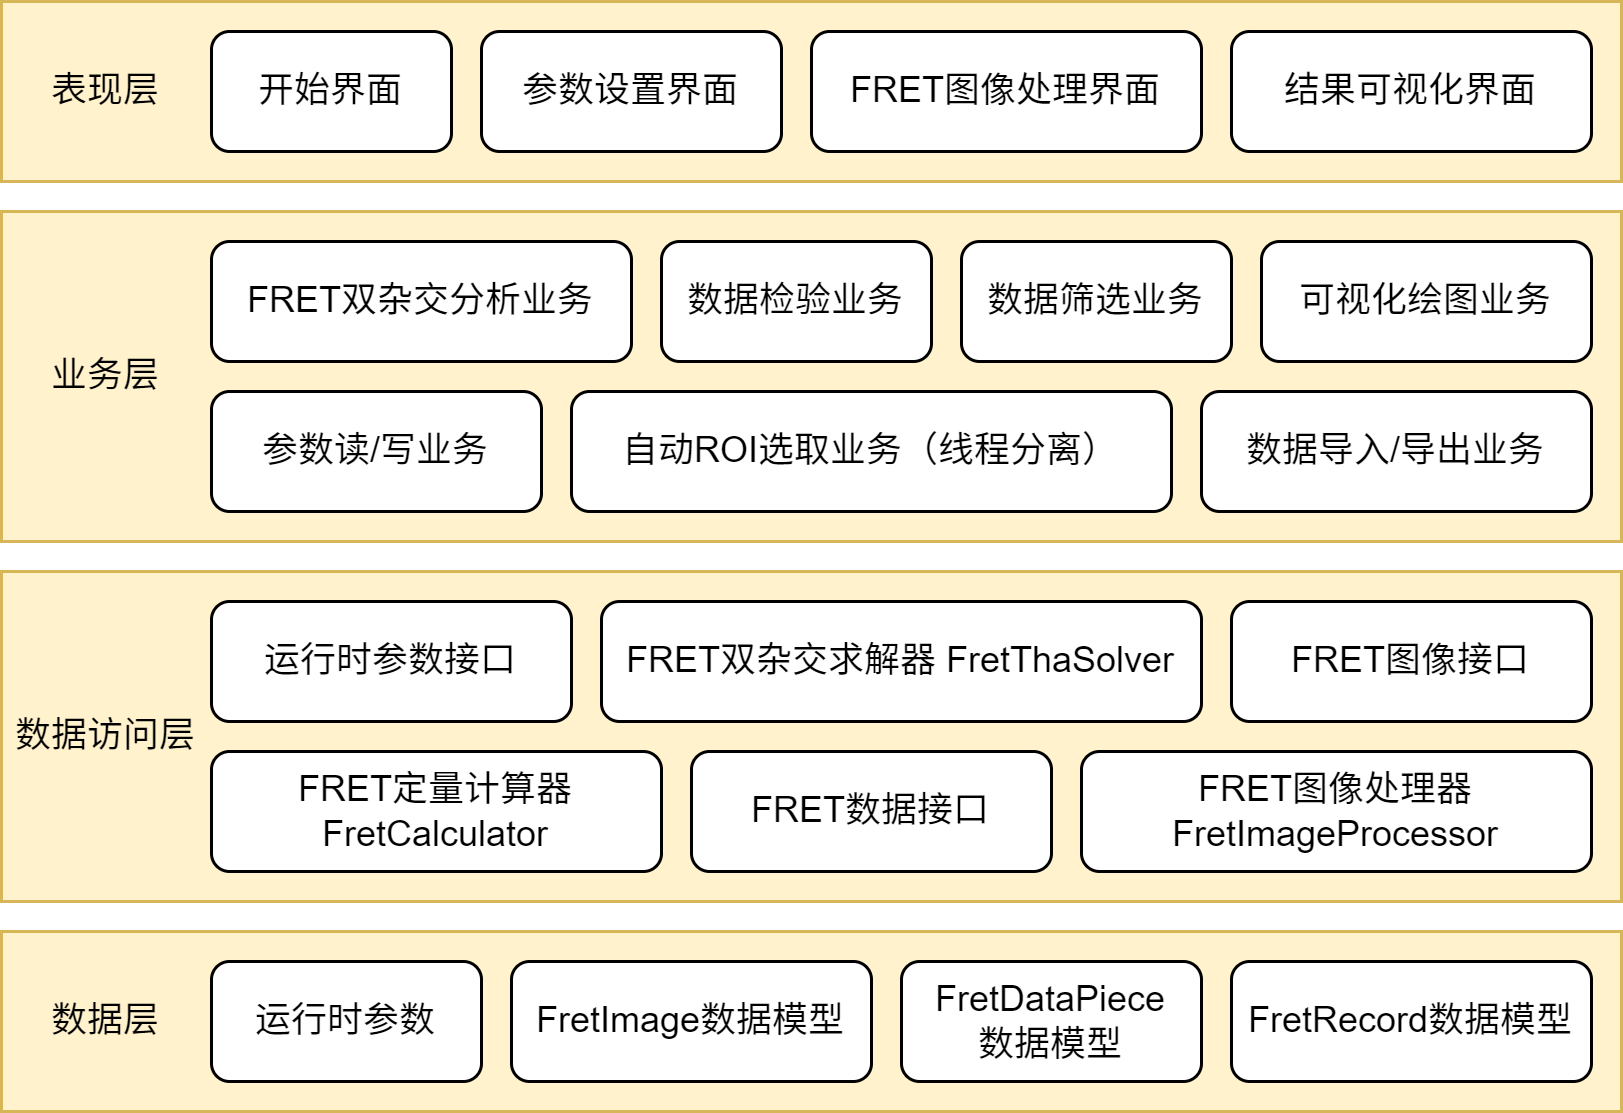
\includegraphics[width=0.9\linewidth]{../figures/2/2_Fretha架构.png}
    \caption{Fretha软件总体架构}
    \label{fig:fretha_arch}
\end{figure}

表现层(Presentation Layer)处于整个架构的最上层,是用户与系统进行交互的主要界面。
表现层通过QtCreator静态构建结合QML动态创建,负责接收用户输入的操作和数据,并以直观、友好的方式展示系统的处理结果。
表现层主要包括开始界面、参数设置界面、FRET图像处理界面、结果可视化界面等。
Fretha通过表现层的设计约束了用户的操作流程和操作规范,标准化和规范化了FRET双杂交分析数据处理的过程。

业务层(Business Logic Layer)是整个架构的核心逻辑处理部分,承担着具体模块功能和其对应的业务逻辑的实现。
业务层接收来自表现层的请求,根据预设的业务逻辑对数据进行处理和转换。
Fretha的业务层封装了包括参数读/写业务、数据检验业务、自动ROI选取业务、数据导入/导出业务、FRET双杂交分析业务、可视化绘图业务等。

数据访问层(Data Access Layer)实现对数据的访问和操作,将业务层与数据层进行隔离。
业务层通过调用数据访问层提供的接口来获取和操作数据,无需关心数据的具体存储方式和位置。
通过设置数据访问层,能够使得在复杂的业务处理时避免对数据的直接操作和影响,从而提高了数据存储的安全性。
Fretha的数据访问层包括FRET图像数据访问、FRET数值数据访问和FRET双杂交数据访问的接口。
特别地,在数据访问层还包括FRET定量计算器和FRET图像处理器、FRET双杂交求解器等,它们除了可以作为数据访问层的接口,还可以完成FRET计算分析作为业务层的业务逻辑处理单元,这样的设计减少了业务层设计的复杂度,提高了系统的可维护性和可扩展性。

最后是数据层(Data Layer),作为架构的最底层,数据层负责存储系统的所有数据。
Fretha数据层包括系统静态数据、FretImage模型、FretDataPiece模型和FretRecord模型。
系统静态数据是在软件运行时的环境参数,只需要在指定步骤运行前提前设置好即可,如成像参数、文件目录等。
FretImage、FretDataPiece和FretRecord用来存储和计算各种动态数据。
在FRET双杂交分析数据处理中,一组FRET三通道图像中可以提取并计算出若干条FRET数据,由若干条FRET数据作为一个批次只能解析出一条FRET双杂交分析结果。
因此,在设计上三种数据实体类型存在关联关系,FretImage和FretDataPiece之间存在一对多的关系,FretDataPiece和FretRecord之间存在一对多关系,如图 \ref{fig:fretha_data_relations} 所示。
\begin{figure}[hbtp]
    \centering
    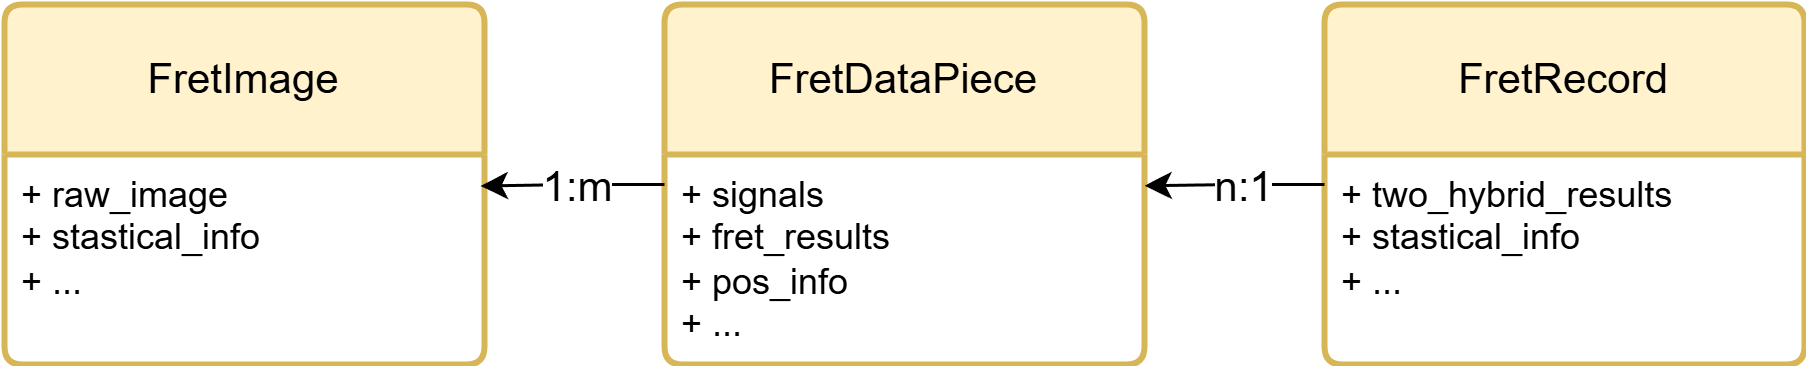
\includegraphics[width=1\linewidth]{../figures/2/2_Fretha数据层对应关系.png}
    \caption{Fretha数据层实体关联关系图}
    \label{fig:fretha_data_relations}
\end{figure}

\subsection{开发技术选型}
\ifshowtext
Qt是目前最流行的跨平台应用程序和 UI 开发框架之一,广泛应用于桌面、嵌入式和移动设备等领域。
Qt提供了可靠的C++类库,提供了良好的跨桌面和嵌入式操作系统的移植性,包括:
\begin{enumerate}
  \item 图形用户界面(Graphics User Interface, GUI):提供了按钮、文本框、对话框等完整的控件,以及支持控件的自定义;
  \item 多线程:方便开发者管理线程,数据和对象,且基于信号和槽机制实现了线程间的安全通信;
  \item OpenGL支持:可以在构建支持硬件加速的高性能可视化应用程序,提高对系统资源的利用。
\end{enumerate}
Qt 5.15.2是Qt官方发布的长期支持(Long Term Support, LTS)版本,本文选择Qt 5.15.2作为Fretha的开发框架。

OpenCV(Open source computer vision library)是一个跨平台开源计算机视觉库。
它轻量级且高效,C++版本由一系列C函数和C++类构成,同时提供了Python、MATLAB等语言的接口。
OpenCV 提供了大量的计算机视觉算法和图像处理工具,广泛应用于图像和视频的处理、分析以及机器学习领域,主要提供的功能库包括:
\begin{enumerate}
  \item 图像处理:提供了经典的图像滤波、边缘检测、颜色空间转换、形态学操作、特征提取等算法;
  \item 视频分析: 视频捕捉、运动分析、物体检测与追踪等;
  \item 机器学习与人工智能: OpenCV 正在不断完善对深度学习和人工智能技术的支持,如人脸识别、目标检测、图像分类等方法。
\end{enumerate}
OpenCV 的很多方法都经过高度优化,支持硬件级别的加速,因此在处理复杂计算功能时具备高性能。
鉴于这些优势,OpenCV 被选为 Fretha 图像处理模块的核心技术方案。

Dlib提供了和机器学习、数值计算、图模型算法、图像处理等领域相关的一系列功能,广泛应用于工业界和学术界,包括机器人,嵌入式设备等高性能计算环境。
L-FRET方法的参数拟合计算是一个非线性约束优化问题,Dlib能够高效地完成求解计算。
Dlib整合了梯度优化算法与自适应学习率策略,在保证收敛速度的同时减少了陷入局部最优的风险。
算法实现上,Dlib 结合了牛顿法和类牛顿方法,这种组合既保留了牛顿法的高精度特性,又通过拟牛顿近似提升了计算效率。
在约束优化问题上,还支持通过内点法解决资源分配中的约束问题。
一次,本文选择Dlib作为Fretha的FRET双杂交求解器的计算支持工具。
\fi

\section{FRET算法和后台接口}

\subsection{FRET定量计算器}
FRET定量计算器(FretCalculator)用于处理E-FRET和$3^3$-FRET定量计算,用于将输入的三通道荧光信号转换为定量FRET信息如$E_A$、$E_D$和$R_C$等。
如图 \ref{fig:fretha_calculator} 所示,FRET定量计算器在实例化后需要经过成像参数设置、加载荧光数据、数据校正、数据计算和结果获取等计算步骤,每个步骤需要按照顺序执行,并且在执行时记录运行状态,在获取结果数据之前进行检查来保证数据安全。
\begin{figure}[hbtp]
  \centering
  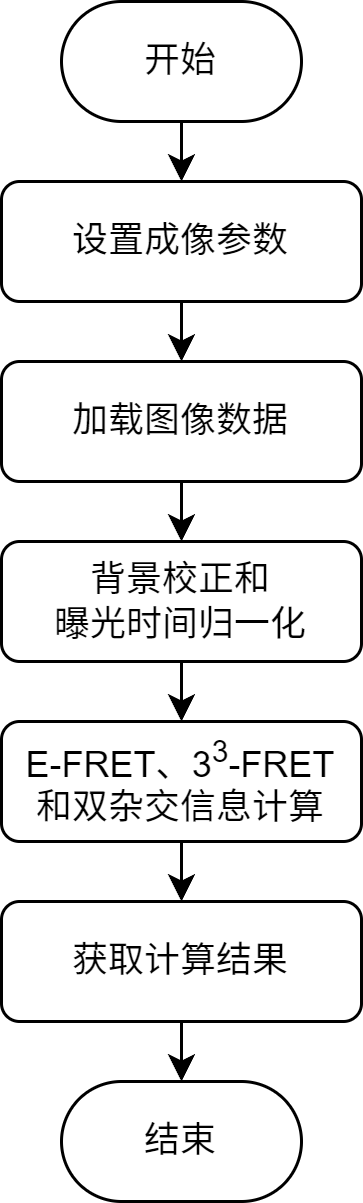
\includegraphics[width=0.25\linewidth]{../figures/2/FRET计算器计算步骤.drawio.png}
  \caption{FretCalculator计算步骤}
  \label{fig:fretha_calculator}
\end{figure}

参数设置中,FretCalculator读取系统静态数据中的成像参数,用于在计算中使用。
通过接口函数加载$I_{DD}$、$I_{DA}$、$I_{AA}$数据到FretCalculator实例的数据成员中,然后
数据校正中,FretCalculator对FRET图像数据进行背景值估计和荧光强度校正,并按照曝光时间进行归一化。
校正后的数据根据E-FRET和$3^3$-FRET方法对荧光强度进行计算,得到FRET定量计算结果$E_D$和$R_C$等。
最后FretCalculator可以返回指定计算结果给调用者。

特别地,除了支持E-FRET和$3^3$-FRET定量计算外,FretCalculator还可以计算L-FRET方法中需要的供体分子数估值$D_{est}$和受体分子数估值$A_{est}$。计算公式如下:
\begin{align}
  M_A/M_D &= G \cdot \frac{\varepsilon_D/\varepsilon_A}{d}, \\
  D_{est} &= d \cdot I_{DD} / (1 - E_D), \\ 
  A_{est} &= \frac{a \cdot (I_{AA} - c\cdot I_{DD})} {M_A/M_D},
\end{align}
其中,$M_A/M_D$是单个供体分子的亮度和单个受体分子亮度之比。

\subsection{FRET图像处理器}
FRET图像处理器(FretImageProcesser)封装了对FRET图像进行定量FRET计算的相关功能,其计算步骤和FretCalculator类似,如图 \ref{fig:fretha_calculator} 所示。
FretImageProcesser接收和返回的数据类型是OpenCV的Mat数据结构,可以方便地存储和处理图像数据和逐像素的FRET图像数据。
FRET图像分析时需要对每个像素点的荧光强度进行计算,对图像数据进行遍历处理。

此外,FRET图像处理器以静态方法的形式提供了FRET图像处理时涉及的一系列算法接口,包括图像预处理、图像分割、特征提取、图像增强等。
所有的算法接口如表 \ref{tab:算法接口} 所示。
运用这些算法,FRET图像处理器支持了对16位原始数据的计算处理能力,以及可视化输出为伪彩图等功能。

\begin{table}[hbtp]
  \centering
  \caption{FRET图像处理库算法接口}
  \label{tab:算法接口}
    \begin{tabular*}{\textwidth}{p{0.3\textwidth}p{0.3\textwidth}p{0.4\textwidth}}
      \toprule[1.5pt]
      { 接口} & { 参数} & { 说明} \\
      \midrule

      \multirow{2}{*}{morphologyClose} & 
      \begin{tabular}[t]{@{}l@{}}
        Mat: 二值化图像 \\ 
        int: 迭代次数
      \end{tabular} & 
      \multirow{2}{*}{形态学闭运算} \\

      \multirow{2}{*}{morphologyOpen} & 
      \begin{tabular}[t]{@{}l@{}}
        Mat: 二值化图像 \\ 
        int: 迭代次数
      \end{tabular} & 
      \multirow{2}{*}{形态学开运算} \\
      
      \multirow{2}{*}{medianFilter} & 
      \begin{tabular}[t]{@{}l@{}}
        Mat: 单通道图像 \\ 
        int: 核大小
      \end{tabular} & 
      \multirow{2}{*}{图像中值滤波} \\

      \multirow{2}{*}{meanFilter} & 
      \begin{tabular}[t]{@{}l@{}}
        Mat: 单通道图像 \\ 
        int: 核大小
      \end{tabular} & 
      \multirow{2}{*}{图像均值滤波} \\
      
      \multirow{3}{*}{gaussianFilter} & 
      \begin{tabular}[t]{@{}l@{}}
        Mat: 单通道图像 \\ 
        int: 核大小 \\
        double: 高斯标准差
      \end{tabular} & 
      \multirow{3}{*}{图像高斯平滑} \\
      
      getBackgroundValue & 
      Mat: 单通道图像 & 
      基于直方图的背景值估计 \\
      
      otsuThreshold & 
      \begin{tabular}[t]{@{}l@{}}
        Mat: 输入图像 \\ 
      \end{tabular} & 
      Otsu自动阈值分割 \\
      
      \multirow{3}{*}{adaptiveThreshold} & 
      \begin{tabular}[t]{@{}l@{}}
        Mat: 输入图像 \\ 
        int: 邻域大小(奇数) \\ 
        double: 阈值偏移量
      \end{tabular} & 
      \multirow{3}{*}{自适应局部阈值分割} \\
      
      applyPseduoColor & 
      Mat: 单通道图像(8位) & 
      伪彩色映射(Jet颜色表) \\
      
      \multirow{2}{*}{applyMask} & 
      \begin{tabular}[t]{@{}l@{}}
        Mat: 输入图像 \\ 
        Mat: 掩膜(二值/同尺寸)
      \end{tabular} & 
      \multirow{2}{*}{图像掩膜操作} \\
      
      minMaxNormalization & 
      Mat: 输入图像 & 
      全局线性归一化 \\
      
      \multirow{3}{*}{mergeChannels} & 
      \begin{tabular}[t]{@{}l@{}}
        Mat: R通道(8位) \\ 
        Mat: G通道(8位) \\ 
        Mat: B通道(8位)
      \end{tabular} & 
      \multirow{3}{*}{多通道图像合并} \\
      \bottomrule[1.5pt]
    \end{tabular*}
\end{table}

\subsection{FRET双杂交求解器}
FRET 双杂交求解器对采集到的 FRET 批数据 $E_D$、$E_A$、$R_C$、$A_{est}$ 和 $D_{est}$ 进行最优化计算,以获取使预测结果与测量结果之间误差最小的$E_{A,max}$、$E_{D,max}$、$n_D / n_A$、$K_{d,EFF}$等参数。求解器从数据模型 FretRecord 中获取批量数据作为数据集,然后分别按照 DC-FRET 方法或 L-FRET 方法进行 FRET 双杂交分析求解。
DC-FRET和L-FRET的双杂交求解算法如下。

求解器首先封装了DC-FRET线性拟合算法。根据公式 \ref{eq:ea_appro} 和 \ref{eq:ed_appro},DC-FRET拟合斜率时截距项为0。以参数$E_{A,max}$的拟合过程为例,其线性方程形式为
\begin{equation}
    E_D = E_{A,max}\cdot R_C ,
\end{equation}
其中,$E_D$是自变量,$R_C$是自变量,$E_{A,max}$是斜率。线性拟合的目标是找到合适的参数$E_{A,max}$,使得方程预测的$E_D$值与实际观测到的$E_D$值之间的误差尽可能小。
通常使用最小二乘法,其原理是最小化观测值与预测值之间的误差平方和$S$,即
\begin{equation}
    S=\sum^{n}_{i=1}(E_{D_i}-(E_{A,max}R_{C_i}))^2 ,
\end{equation}
其中,$n$是数据点的数量,$R_{C_i}$和$E_{D_i}$分别是第i个数据点的自变量和因变量的值。
首先,对$S$关于$E_{A,max}$求偏导:
\begin{align}
      S=\sum_{i = 1}^{n}(E_{D_i}^{2}-2E_{A,max}R_{C_i}E_{D_i} + E_{A,max}^{2}R_{C_i}^{2}), \\
      \frac{\partial S}{\partial E_{A,max}}=\sum_{i = 1}^{n}(-2R_{C_i}E_{D_i} + 2E_{A,max}R_{C_i}^{2}),
\end{align}
为了找到$S$最小的$E_{A,max}$值,令$\frac{\partial S}{\partial E_{A,max}}=0$:
\begin{align}
      \sum_{i = 1}^{n}(-2R_{C_i}E_{D_i} + 2E_{A,max}R_{C_i}^{2}) = 0, \\
    -2\sum_{i = 1}^{n}R_{C_i}E_{D_i}+2E_{A,max}\sum_{i = 1}^{n}R_{C_i}^{2}=0,
\end{align}
最后求解$E_{A,max}$:
\begin{equation}
        E_{A,max}=\frac{\sum_{i = 1}^{n}R_{C_i}E_{D_i}}{\sum_{i = 1}^{n}R_{C_i}^{2}}. \label{eq:linear_fit_quick}
\end{equation}
公式 \ref{eq:linear_fit_quick} 给出了线性拟合求解$E_{A,max}$的解析公式,应用类似方法可直接计算斜率$E_{A,max}$和$E_{D,max}$,从而避免了基于迭代的线性拟合求解算法的消耗。

Langmiur模型具有非线性和参数复杂性,无法通过解析式求解其中的参数。因此,求解器通过引入Dlib计算库进行复杂的参数拟合。
如代码 \ref{code:data_type} 所示,求解器设计了拟合计算中涉及到的数据类型:
(1)ColumnVector类型用于存储双精度浮点数的列向量,在后续的计算和优化过程中承载参数向量和中间计算结果;
(2)ExperimentalData结构体存储实验采集到的数据集,包含四个std::vector<double>类型的成员变量:aest存储受体分子数估值$A_{est}$,dest存储供体分子数估值$D_{est}$,ea\_measure存储$E_A$的测量值,ed\_measure存储$E_D$测量值。
\begin{lstlisting}[language=C++, caption={数据类型}, label={code:data_type}]  
// 定义列向量类型
typedef Dlib::matrix<double, 0, 1> ColumnVector;

// 定义数据结构体,用于存储实验数据
struct ExperimentalData {
    std::vector<double> aest;
    std::vector<double> dest;
    std::vector<double> ea_measure;
    std::vector<double> ed_measure;
};
\end{lstlisting}
CalculateLoss函数计算模型在整个数据集上的整体损失,作为优化的目标函数。
在函数内,首先对于ExperimentalData实例中的每个向量中的每个数据,计算出$E_A$或$E_D$预测值,然后求得与实际值之间的误差的平方,最后将误差累加并返回,其实现代码如下:
\begin{lstlisting}[language=C++, caption={误差计算函数}, label={code:error_calculate}]
// 计算整体损失
double CalculateLoss(const ExperimentalData& data, const ColumnVector& parameters) {
    double total_error = 0.0;
    for (size_t i = 0; i < data.aest.size(); ++i) {
        double d_free = ((data.dest[i] - parameters(0) - data.aest[i] * parameters(1)) + std::sqrt(std::pow(data.dest[i] - parameters(0) - data.aest[i] * parameters(1), 2) + 4 * parameters(0) * data.dest[i])) / 2;
        double a_free = data.aest[i] - (data.dest[i] - d_free) / parameters(1);
        double ea_pred = parameters(2) * d_free / (d_free + parameters(0));
        double ed_pred = parameters(3) * a_free / (a_free + parameters(0) / parameters(1));

        total_error += CalculateError(data.ea_measure[i], ea_pred) + CalculateError(data.ed_measure[i], ed_pred);
    }
    return total_error;
}
\end{lstlisting}
TwoHybridSolver函数实现了整个拟合过程,并向外提供调用接口,如代码 \ref{code:two_hybrid_solver} 所示。
拟合过程中,首先设置$K_{d,EFF}$、$n_D/n_A$、$E_{A,max}$和$E_{D,max}$的拟合初值为 1、1、0.5 和 0.5, 存储到 {starting\_point}中。
使用 {Dlib} 库中的 {find\_min\_using\_approximate\_derivatives} 函数进行优化,采用一种拟牛顿法 {dlib::bfgs\_search\_strategy()}搜索策略算法,在参数空间中寻找目标函数的最小值,并使用 {dlib::objective\_delta\_stop\_strategy(1e - 7)} 作为停止策略,当两次拟合后参数的变化小于 $10^{-7}$ 时,认为此时的结果已收敛,停止优化过程。
最后,函数返回 {starting\_point} 存储的优化后的参数。
\begin{lstlisting}[language=C++, caption={双杂交求解器}, label={code:two_hybrid_solver}]
  
  // 双杂交求解器,进行参数拟合
  ColumnVector TwoHybridSolver(const std::vector<double>& aest_data, const std::vector<double>& dest_data, const std::vector<double>& ea_measure_data,const std::vector<double>& ed_measure_data) {
      // 初始化参数起始点和数据
      ColumnVector starting_point(4);
      starting_point = 1, 1, 0.5, 0.5;
      ExperimentalData data = {aest_data, dest_data, ea_measure_data, ed_measure_data};

      // 定义目标函数包装器
      auto objective_wrapper = [&data](const ColumnVector& parameters) {
          return ObjectiveFunction(parameters, &data);
      };
  
      // 使用 Dlib 进行优化
      Dlib::find_min_using_approximate_derivatives(Dlib::bfgs_search_strategy(), Dlib::objective_delta_stop_strategy(1e-7), objective_wrapper, starting_point, -1, 0.01);

      return starting_point;
  }
\end{lstlisting}  

\section{功能模块的实现}

\subsection{成像参数设置模块}
\ifshowtext
FRET定量分析中,在数据处理前需要设置好FRET定量计算过程中必须的参数,设置成像过程时的成像参数至关重要。
成像参数设置模块的界面如图 \ref{fig:参数设置页界面} 所示,包括了FRET成像参数的设置和保存功能。

FRET成像参数在Fretha中以静态参数保存在软件内存中,是数据处理时的环境参数。其中,$a$、$b$、$c$、$d$、$G$、$k$和$\varepsilon_{A}/\varepsilon_{D}$是FRET成像系统的光学参数,在前文中已介绍;ExpTimeAA、ExpTimeDD和ExpTimeDA是成像时三个探测通道的曝光时间,在FRET定量计算时需要根据曝光时间参数在各个通道归一化,然后才能进行计算。
Fretha中包括的所有成像参数如表 \ref{tab:fretha_param_list} 所示。

\begin{table}[htb]
  \centering
  \caption[FRET成像参数]{FRET成像参数}
  \label{tab:fretha_param_list}
    \begin{tabular*}{\textwidth}{cp{8cm}lc}
      \toprule[1.5pt]
      { 参数} & { 说明} & { 意义范围} & {单位} \\
      \midrule
      $a$ & 受体激发的串扰系数 & $(0,1)$ & 无\\
      $b$ & 受体发射的串扰系数 & $(0,1)$ & 无\\
      $c$ & 供体发射的串扰系数 & $(0,1)$ & 无\\
      $d$ & 供体激发的串扰系数 & $(0,1)$ & 无\\
      $G$ & 供体猝灭和受体荧光增强的比值         & $(0,+\infty)$ & 无\\
      $k$ & 受体浓度和供体浓度相同时的荧光比值 & $(0,+\infty)$ & 无\\
      {$\varepsilon_{A}/\varepsilon_{D}$} & 供受体在激发光条件下的消光系数之比 & {$(0,+\infty)$} & {无}\\
      \text{ExpTimeDD} & DD通道下的成像曝光时间 & $(0,+\infty)$ & 毫秒(ms)\\
      \text{ExpTimeDA} & DA通道下的成像曝光时间 & $(0,+\infty)$ & 毫秒(ms)\\
      \text{ExpTimeAA} & AA通道下的成像曝光时间 & $(0,+\infty)$ & 毫秒(ms)\\
      \bottomrule[1.5pt]
    \end{tabular*}
\end{table}
\begin{figure}[hbtp]
  \centering
  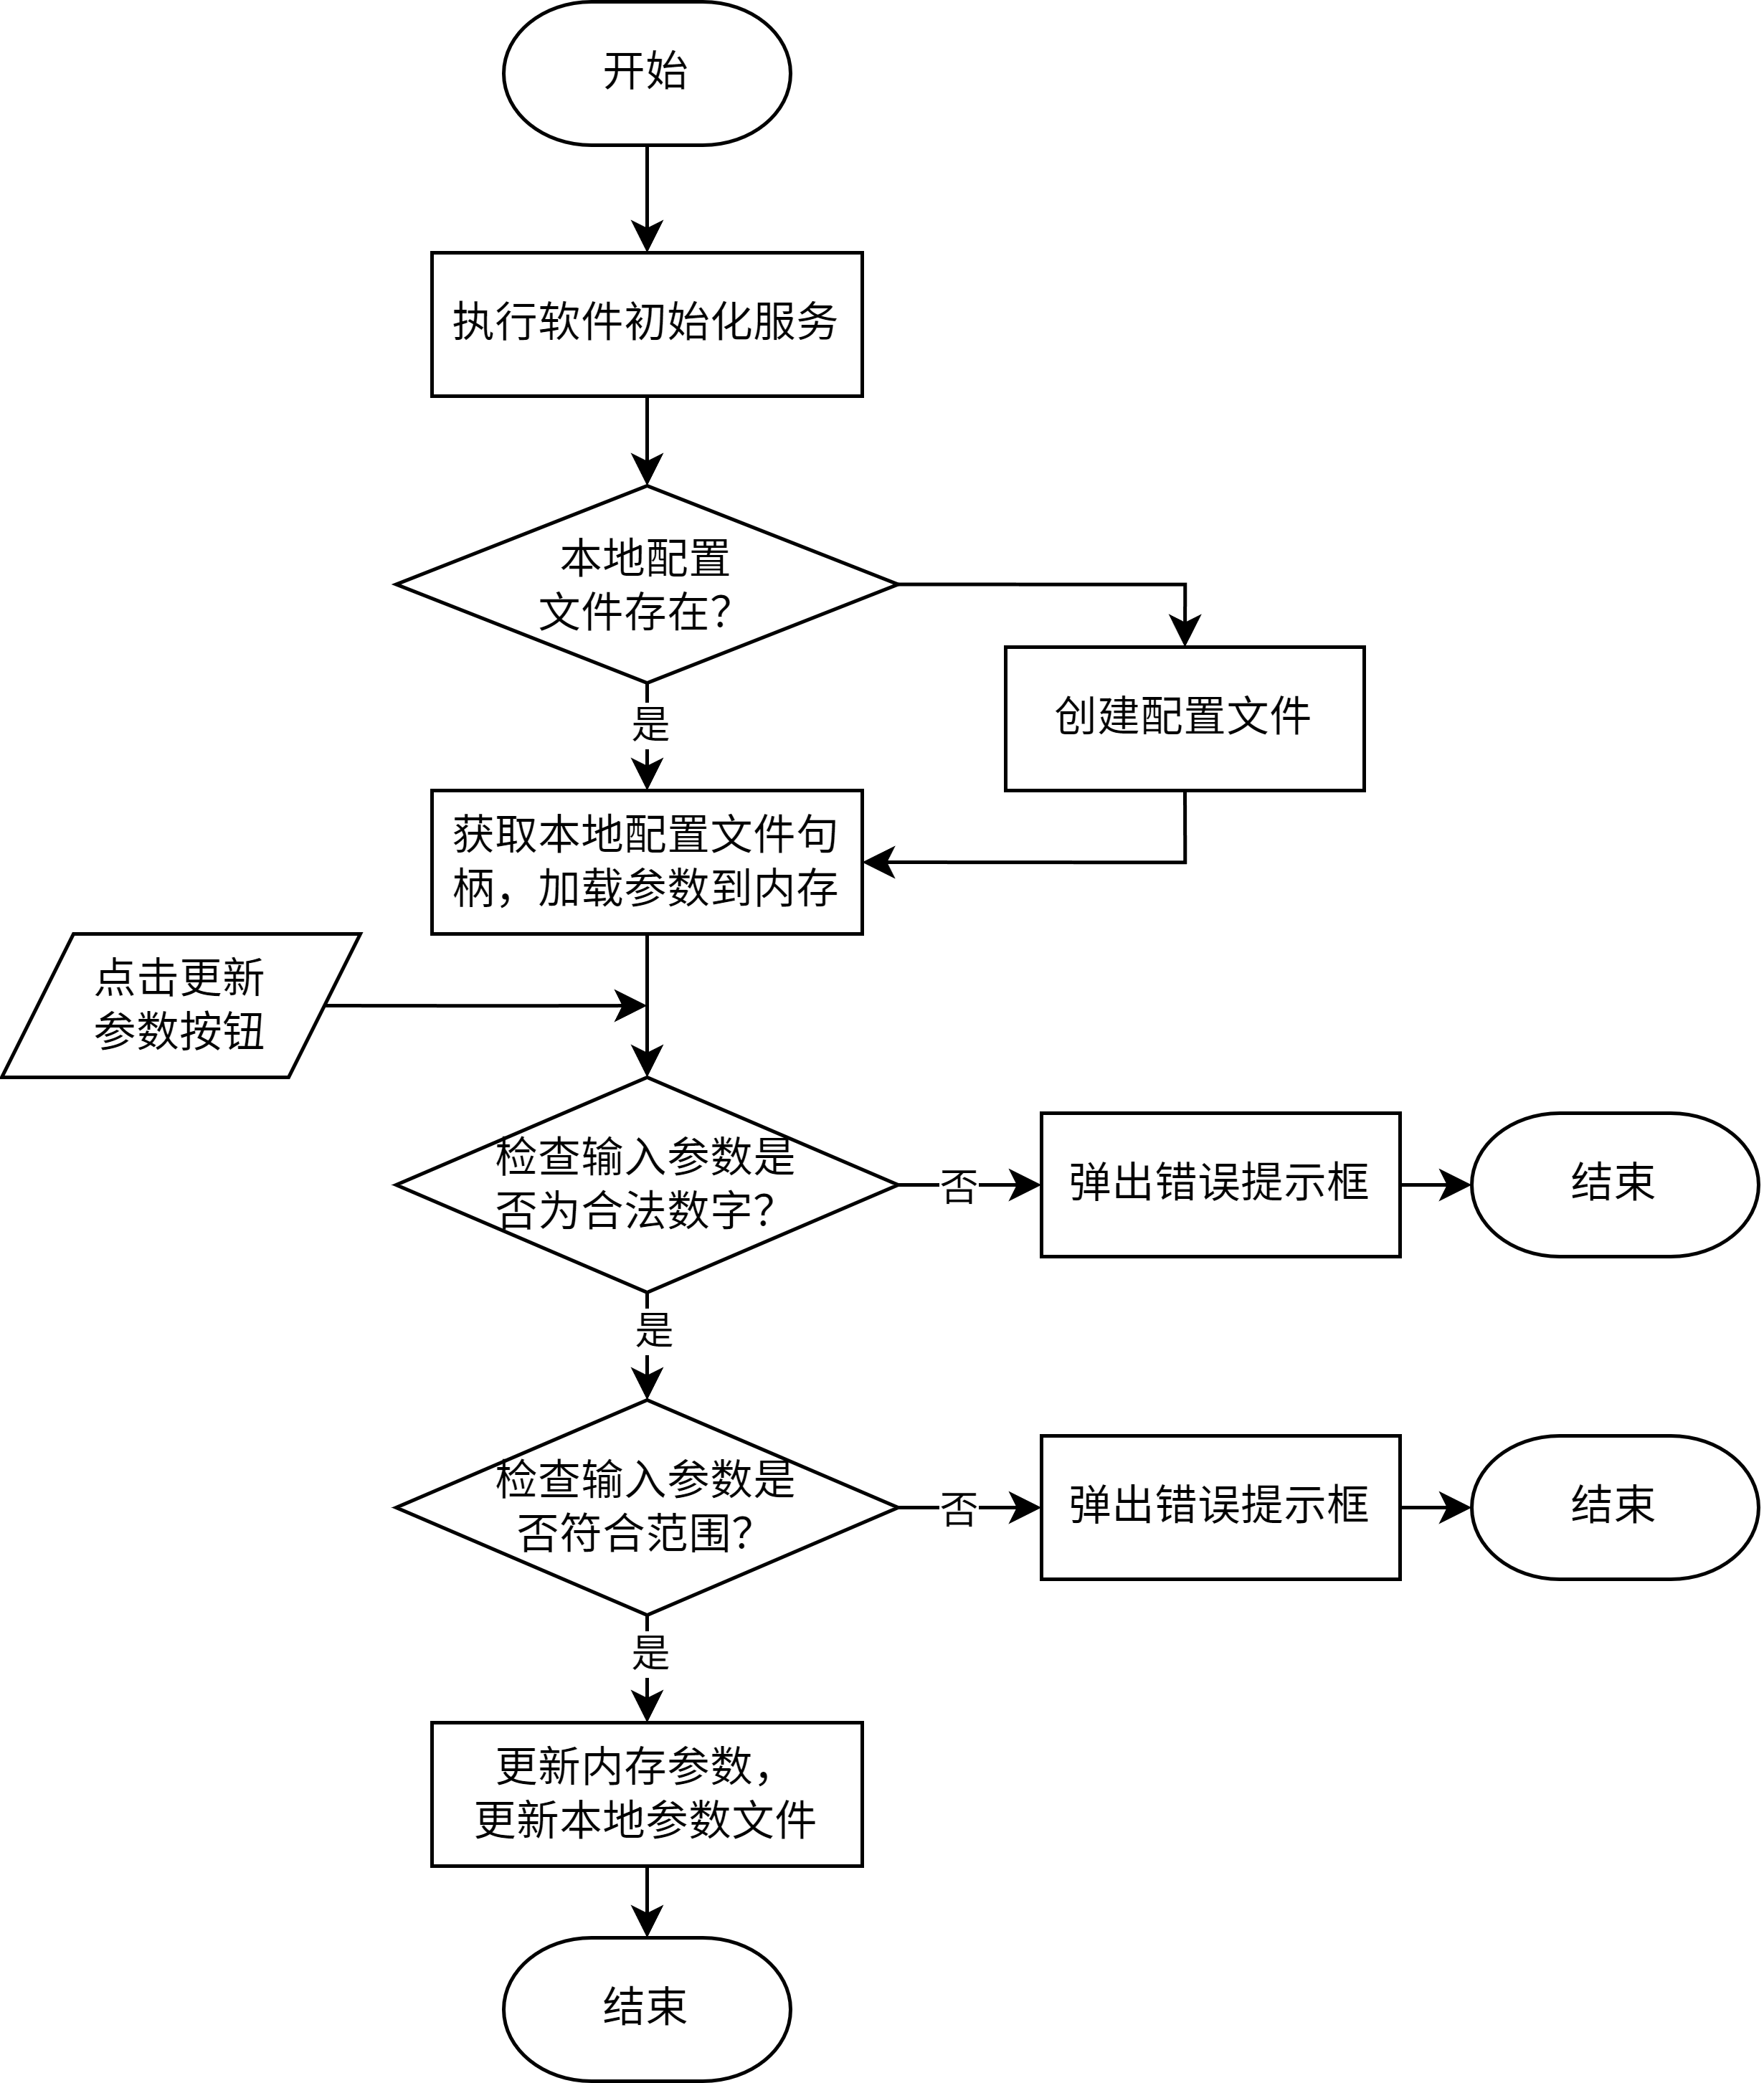
\includegraphics[height=0.9\linewidth]{../figures/2/2_成像参数设置模块业务流程.png}
  \caption{参数设置模块业务流程}
  \label{fig:fretha_param_module_flow}
\end{figure}
参数设置的主要业务流程如图 \ref{fig:fretha_param_module_flow} 所示,遵循如下原则:(1)所有参数一同更新,避免因参数不匹配导致的数据处理错误;(2)每个参数需要在其有意义的范围内,避免无意义的值。
FRET成像参数是一批参数,参数间存在依赖关系,比如测定参数$G$、$k$、$\varepsilon_{A}/\varepsilon_{D}$时需要计算敏化发射荧光$F_C$,根据公式 \ref{eq:fc} 所示,$F_C$的确定与$a$、$b$、$c$、$d$密切相关,因此依赖参数$a$、$b$、$c$、$d$。
强制所有参数一同更新可以避免用户单独设置某一参数而导致参数之间不匹配等问题。
因此,在点击“更新参数”按钮时,若无法从界面中的每个参数输入框都解析到合法的数字,那么本次更新参数就会失败。

FRET成像参数一般比较稳定,一般2到3个月才需要重新测量,因此需要持久化到本地,以供多次处理数据时使用。
Fretha的本地参数文件保存为可执行程序同级目录下的“config.ini”中。在软件初始化阶段,会自动检测并应用本地配置文件中的参数。
用户可通过保存多套配置文件,在使用时替换目标配置文件,快速进行参数配置的切换。
\fi

\subsection{数据检验模块}
\label{sec:数据检验模块}

FRET双杂交分析需要处理一批FRET图像文件,因此需要对输入数据的完备性进行检验识别。
该模块的作用有以下两个方面:一方面通过模式识别FRET合法数据,避免了异常输入导致的运行错误;
另一方面,在这一模块会将FRET批数据的视野子文件夹进行解析和类型识别,为后续数据处理提供对子文件夹的不同操作。

Fretha的数据识别检验模块匹配识别FRETScope的数据格式,从而保证数据处理能够正常开始。
如图 \ref{fig:fretscope_data_struct} 所示,FRETScope的数据结构由上层到下层依次为:
\begin{enumerate}
  \item 批数据根目录:存放所有视野子目录和数据文件;
  \item 视野子目录:存放一个视野的三通道图片和参数文件;
  \item 图片数据和参数文件。
\end{enumerate}

\begin{figure}[htbp]
    \centering
    \includegraphics[height=0.5\linewidth]{../figures/2/2_FRETScopeII数据格式.drawio.png}
    \caption{FRETScope数据文件结构}
    \label{fig:fretscope_data_struct}
\end{figure}

数据检验业务的流程如图 \ref{fig:fretha_data_check_flow} 所示。
其中,检查子文件夹类型是通过图 \ref{fig:fretscope_data_struct} 进行匹配的,当且仅当子文件夹中同时存在“DA.tif”、“DD.tif”和“AA.tif”图片文件时,当前子文件夹会被识别为FRET视野,并在视野表格模型中记录。
其他情况的子文件夹会被记作“Unknown”文件夹,在后续FRET图像处理或者自动处理中被跳过。
这种检查还会对图像数据是否可读进行检查。
\begin{figure}[htbp]
    \centering
    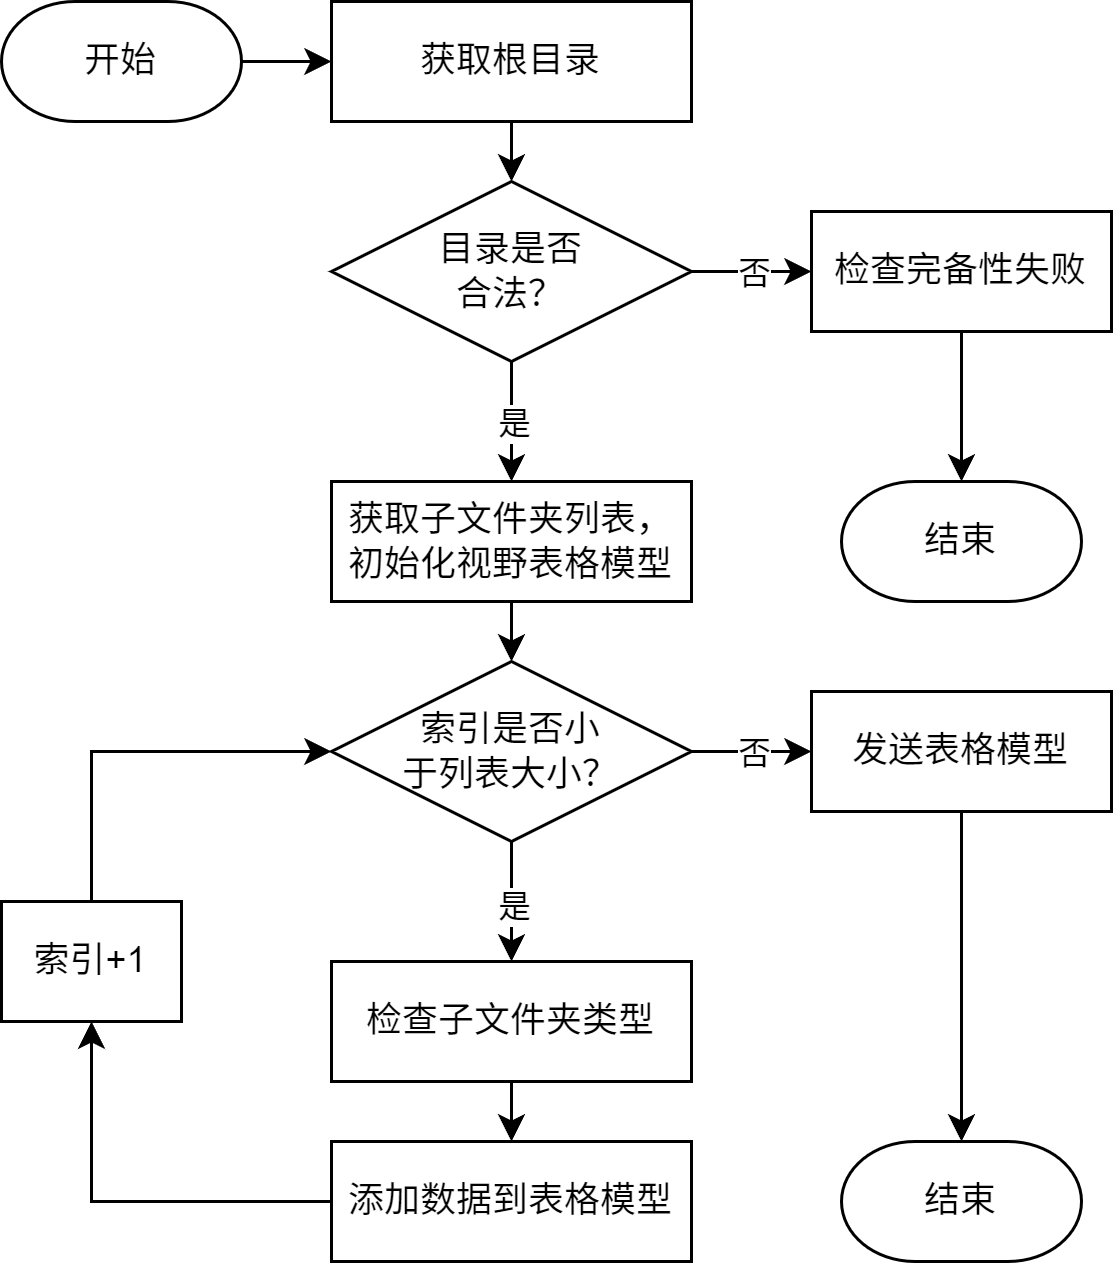
\includegraphics[width=0.65\linewidth]{../figures/2/2_数据完备性检验业务.drawio.png}
    \caption{Fretha数据检验业务主流程图}
    \label{fig:fretha_data_check_flow}
\end{figure}

\subsection{FRET图像处理模块}
\label{sec:FRET图像处理模块}
FRET图像处理模块是对FRET三通道图像进行ROI标注等图像处理分析的模块,其界面如图 \ref{fig:fretha_imageprocess_ui} 所示:
\begin{figure}[htbp]
    \centering
    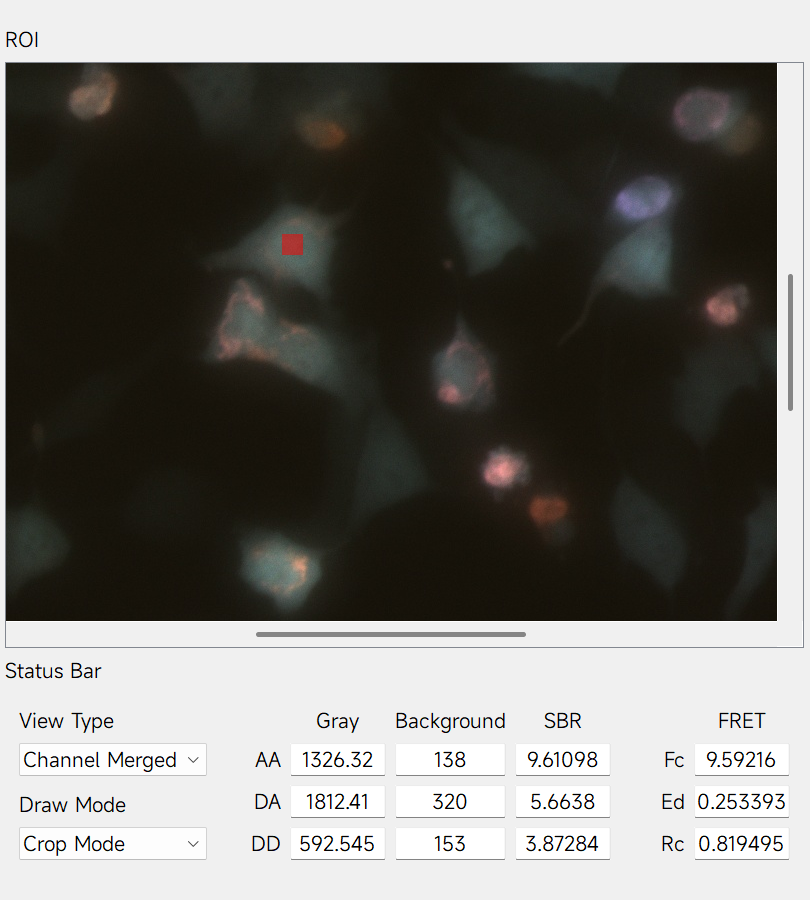
\includegraphics[width=0.75\linewidth]{../figures/2/2_图像处理模块界面.png}
    \caption{Fretha图像处理模块界面}
    \label{fig:fretha_imageprocess_ui}
\end{figure}
在FRET图像处理工作里,手动选取感兴趣区域ROI是一个基础且关键的操作,它能帮助分析人员聚焦于特定区域,进行更精确的数据处理与分析。
为实现图像处理过程中 ROI 的手动选取功能,Fretha 借助 Qt 框架提供的 QGraphicsView 类,开发了自定义的 FretGraphicsView 类。
QGraphicsView 是 Qt 用于可视化和交互处理二维图形场景的重要类,具备丰富的功能和良好的可扩展性,为 FretGraphicsView 的实现提供了有力支撑。

FretGraphicsView 类中设计了一个基于QRectItem的ROI 成员,它能够在视图中直观呈现 ROI 的大小和位置,方便用户确认所选区域。
设定ROI的绘制模式为“Crop Mode”截取模式时,此时会根据鼠标和ROI边框的位置决定鼠标的编辑功能,包括ROI的创建、移动、缩放等操作。
切换绘制模式为“Stamp”邮戳模式,ROI的大小将会被固定,从而快速圈选多个大小一致的ROI。

Fretha的状态栏中提供了视图类型切换选项,在数据处理中可以辅助圈点,支持的视图类型如表 \ref{tab:fretha_viewtype_list} 所示。
\begin{table}[htbp]
  \centering
  \caption[FRET图像视图类型]{FRET图像视图类型}
  \label{tab:fretha_viewtype_list}
    \begin{tabular}{cc}
      \toprule[1.5pt]
      {视图名} & {说明} \\
      \midrule
      Channel Merged & 三通道归一合成图 \\
      DD Normalized & DD通道的归一化增强图 \\
      DA Normalized & DA通道的归一化增强图 \\
      AA Normalized & AA通道的归一化增强图 \\
      $R_C$ Pseudo & $R_C$逐像素数值伪彩图 \\
      $E_D$ Pseudo & $E_D$逐像素数值伪彩图 \\
      \bottomrule[1.5pt]
    \end{tabular}
\end{table}
归一化增强图包括DD、DA、AA通道分别归一化的增强视图以及三通道归一化合成图。
由于FRET成像系统的相机的量程为$[0,65535]$,计算机显示渲染机制里显示会将65535的灰度值设为白色,而0的灰度值设为黑色,这样会导致图像的对比度低而不利于观察。
通过表 \ref{tab:算法接口} 中的 minMaxNormalization 算法,可以对图像进行全局线性归一化,从而增强图像的对比度。
三通道归一化合并图则是将三个通道的归一化增强图分别作为RGB色彩通道合并成一幅彩色图像,以便于用户直观地观察三通道的信号分布,无需切换通道。
通过FretImageProcessor进行逐像素FRET计算得到$E_D$和$R_C$逐像素矩阵,然后归一化后赋予伪彩,得到用于显示FRET信息的逐像素伪彩图。

Fretha状态栏能够清晰展示当前视野及ROI的状态信息,如当前视野的三通道背景灰度值、ROI信号的三通道信号背景比等,还可以显示使用当前ROI提供的扣除背景灰度值后的$I_{DD}$、$I_{DA}$和$I_{DD}$,其中所有显示内容如表 \ref{tab:fret_statusbar_list} 所示。
FretGraphicsView 通过自定义鼠标释放事件的信号,实现了与数据访问层的数据交互。
当用户完成 ROI 选取并释放鼠标时,FretGraphicsView 会将 ROI 的坐标和大小信息传递给数据访问层。
数据访问层依据当前视野索引,从数据模型中读取相应的三通道图像文件,并且从ROI信息提取FRET信号。
在获得了$I_{DD}$、$I_{DA}$和$I_{DD}$后,Fretha后台会自动扣除每个通道的背景灰度,然后根据公式 \ref{eq:fc},调用后台的FretCalculator计算出敏化发射的荧光强度$F_C$、$E_D$,$R_C$,并显示在状态栏中,方便用户获取处理结果,为ROI的保留和移除提供判断依据。
这种基于 QGraphicsView 扩展的设计,有效提升了 ROI 选取的灵活性和准确性。 

\begin{table}[htbp]
  \centering
  \caption[FRET圈点状态栏显示内容]{FRET圈点状态栏显示内容}
  \label{tab:fret_statusbar_list}
      \begin{tabular}{cc}
      \toprule[1.5pt]
      {信息} & {说明} \\
      \midrule
      DD通道信号 & DD通道的ROI内灰度均值 \\
      DA通道信号 & DA通道的ROI内灰度均值 \\
      AA通道信号 & AA通道的ROI内灰度均值 \\
      DD通道背景 & DD通道的视野背景灰度值 \\
      DA通道背景 & DA通道的视野背景灰度值 \\
      AA通道背景 & AA通道的视野背景灰度值 \\
      DD通道SBR & DD通道的信号背景比 \\
      DA通道SBR & DA通道的信号背景比 \\
      AA通道SBR & AA通道的信号背景比 \\
      $F_C$ & 敏化发射的荧光强度 \\
      $E_D$ & 供体视角的表观FRET效率 \\
      $R_C$ & 受体与供体的浓度比 \\
      \bottomrule[1.5pt]
    \end{tabular}
\end{table}

\subsection{数据管理模块}
\label{sec:数据管理模块}

数据管理模块支持对数据的实时操作,可以对于图像处理模块获得的数据,进行异常数据筛选、数据追踪、数据导入、数据导出、计算入口等数据管理控制功能。

一条数据类型FretDataPiece中包含数据如表 \ref{tab:数据项内容定义} 所示。
可以看出,FretDataPiece包含了一个ROI对应的所有原始信息,如ROI的位置、大小、信号强度、视野等;
同时,还包含了计算后的$E_D$、$E_A$、$R_C$、$1/R_C$等中间参数,可以直接被用于后续的数据处理。

\begin{table}[htbp]
  \centering
  \caption{FretDataPiece数据类型}
  \label{tab:数据项内容定义}
    \begin{tabular}{cc}
      \toprule[1.5pt]
      {信息} & {说明} \\
      \midrule
      $I_{DD}$ & ROI在DD通道扣除背景后的信号强度 \\
      $I_{DA}$ & ROI在DA通道扣除背景后的信号强度 \\
      $I_{AA}$ & ROI在DD通道扣除背景后的信号强度 \\
      $E_D$ & 根据$I_{DD}$、$I_{DA}$、$I_{AA}$计算的$E_D$ \\
      $R_C$ & 根据$I_{DD}$、$I_{DA}$、$I_{AA}$计算的$R_C$ \\
      $E_A$ & 根据$I_{DD}$、$I_{DA}$、$I_{AA}$计算的$E_A$ \\
      $1/R_C$ & $R_C$的倒数 \\
      $A_{est}$ & 供体分子数的估计值 \\
      $D_{est}$ & 受体分子数的估计值 \\
      $x$ & ROI的横坐标 \\
      $y$ & ROI的纵坐标 \\
      $w$ & ROI的宽度 \\
      $h$ & ROI的高度 \\
      $view$ & ROI隶属的视野\\
      \bottomrule[1.5pt]
    \end{tabular}
\end{table}

为保证数据符合实际物理意义,避免中间变量的异常值对后续计算产生影响,数据管理模块提供了数据筛选功能。
点击“筛选数据”,数据管理模块会对数据根据物理定义和统计学准则进行筛选,剔除异常数据。
具体数据筛选流程实施如下:
\begin{enumerate}
  \item 对$I_{DD}$、$I_{DA}$、$I_{AA}$基于物理约束的初步数据清洗:
    针对各数值型变量 \( x_i \),依据其预设的物理合理区间 \( [L_i, U_i] \) 执行有效性校验。构建如下二元判别函数:
    \begin{equation}
      \delta(x_i) = 
      \begin{cases} 
        1, & x_i \notin [L_i, U_i]  \\
        0, & x_i \in [L_i, U_i]
      \end{cases} ,
    \end{equation}
    当 \( \delta(x_i) = 1 \) 时,判定该数据点为物理意义上的异常值并予以剔除。
  \item 对中间变量$E_D$、$E_A$、$R_C$统计离群点检测:
    对经初步清洗后的数据子集 \( E_D \)、\( E_A \)和$R_C$,分别计算变量的样本均值 \( \mu \) 和样本标准差 \( \sigma \),计算公式如下:
    \begin{equation}
      \mu = \frac{1}{n}\sum_{i=1}^n x_i, \quad \sigma = \sqrt{\frac{1}{n - 1}\sum_{i=1}^n (x_i - \mu)^2}.
    \end{equation}
    采用3σ准则设定离群阈值,即构建判别区间 \( [\mu - 3\sigma, \mu + 3\sigma] \)。超出该区间的观测值均判定为统计离群点并剔除。
\end{enumerate}

数据导出用于保存数据处理时的ROI信息。
在完成FRET图像处理和ROI绘制选取后,需要保存ROI的结果,以便后续分析或者修改编辑。
在数据管理模块点击“导出数据”按钮,Fretha将会导出数据区记录的所有数据,每一条数据都会按照FretDataPiece定义进行逐列导出,文件格式为CSV文件。
数据导入功能则可以读取Fretha导出的CSV文件,然后解析其中的数据按照FretDataPiece的格式。

点击“添加数据”按钮或者使用快捷键“A”,可以添加当前状态栏中的数据到数据表格中;
点击“删除数据”按钮或者使用快捷键“D”,可以删除数据表格中选中的数据;
点击“清空数据”按钮或者使用快捷键“C”,可以清空数据表格中的所有数据;
点击“开始计算”按钮,软件将调用FretTwoHybridSolver等算法对数据表格中的数据进行FRET双杂交分析求解计算,并将结果显示在结果可视化模块中,然后切换软件界面到结果可视化模块。

在数据表格中点击某一条数据,软件会根据这条数据的位置和形状信息,在图像显示上显示该条数据对应的ROI位置,以方便检查数据处理中标注ROI的错误。
实现这一功能,主要基于Qt提供的信号与槽机制。
将数据中的数据模型被点击的事件信号与 FretGraphicsView 控件中的回调槽函数绑定后,FretGraphicView 模型可以接收到来自所选数据的信息,按照所选数据项中ROI的$x$、$y$、$w$和$h$绘制ROI到FretGraphicsView控件上,并将FretGraphicsView的视角中心移动到所选数据的ROI中心,以便用户更加直观地查看数据的位置和形状。

\subsection{结果可视化模块}
\label{sec:结果可视化模块}
\ifshowtext
FRET双杂交分析的输出结果包含双杂交计算的参数结果与拟合曲线图。
其中,$E_{A,max}$、$E_{D,max}$、$n_D/n_A$、$K_{d,EFF}$等参数以数据框形式展示;
拟合曲线图通过将双杂交理论拟合曲线与实验散点数据同图可视化,实现对拟合效果的直观评估,进而验证FRET双杂交分析结果的可靠性。

结果可视化模块的界面组成如图 \ref{fig:Fretha结果可视化模块界面} 所示,主要包含以下三个功能区域:
\begin{enumerate}
  \item 视图选择:切换FRET双杂交分析算法,更新对应的结果视图;
  \item 图表分析:显示FRET双杂交分析的拟合趋势线和散点图;
  \item 操作按钮:结果保存按钮和返回圈点界面按钮。
\end{enumerate}

点击视图按钮可以切换不同FRET双杂交分析的算法方法的计算结果,更新图表分析区域显示的方法。
在可视化结果展示区域,软件将拟合结果与实验数据同步呈现在同一坐标系中,便于用户进行直接比对。
拟合曲线是基于拟合参数计算得到的理论数据点连接而成的平滑曲线,实验数据则以离散点形式展示,用户可以直观检查拟合计算的效果和误差大小。
可视化界面基于QChart组件作图绘制,根据一批数据(FretDataRecord)的数据范围分布,自动优化坐标轴刻度范围,以提升数据可视化的清晰度。

在 L-FRET 视图模式下,软件集成了数据预处理 BIN 功能,允许用户通过合并供体 - 受体浓度在相同区间的数据进行预处理数据\upcite{供体-受体浓度比}。如图 \ref{fig:Fretha结果可视化模块界面},通过设置界面中数据合并预处理的参数,然后点击“更新”按钮即可应用数据预处理,在L-FRET拟合效果不理想时可以用来优化数据处理结果。
\begin{figure}[htbp]
  \centering
  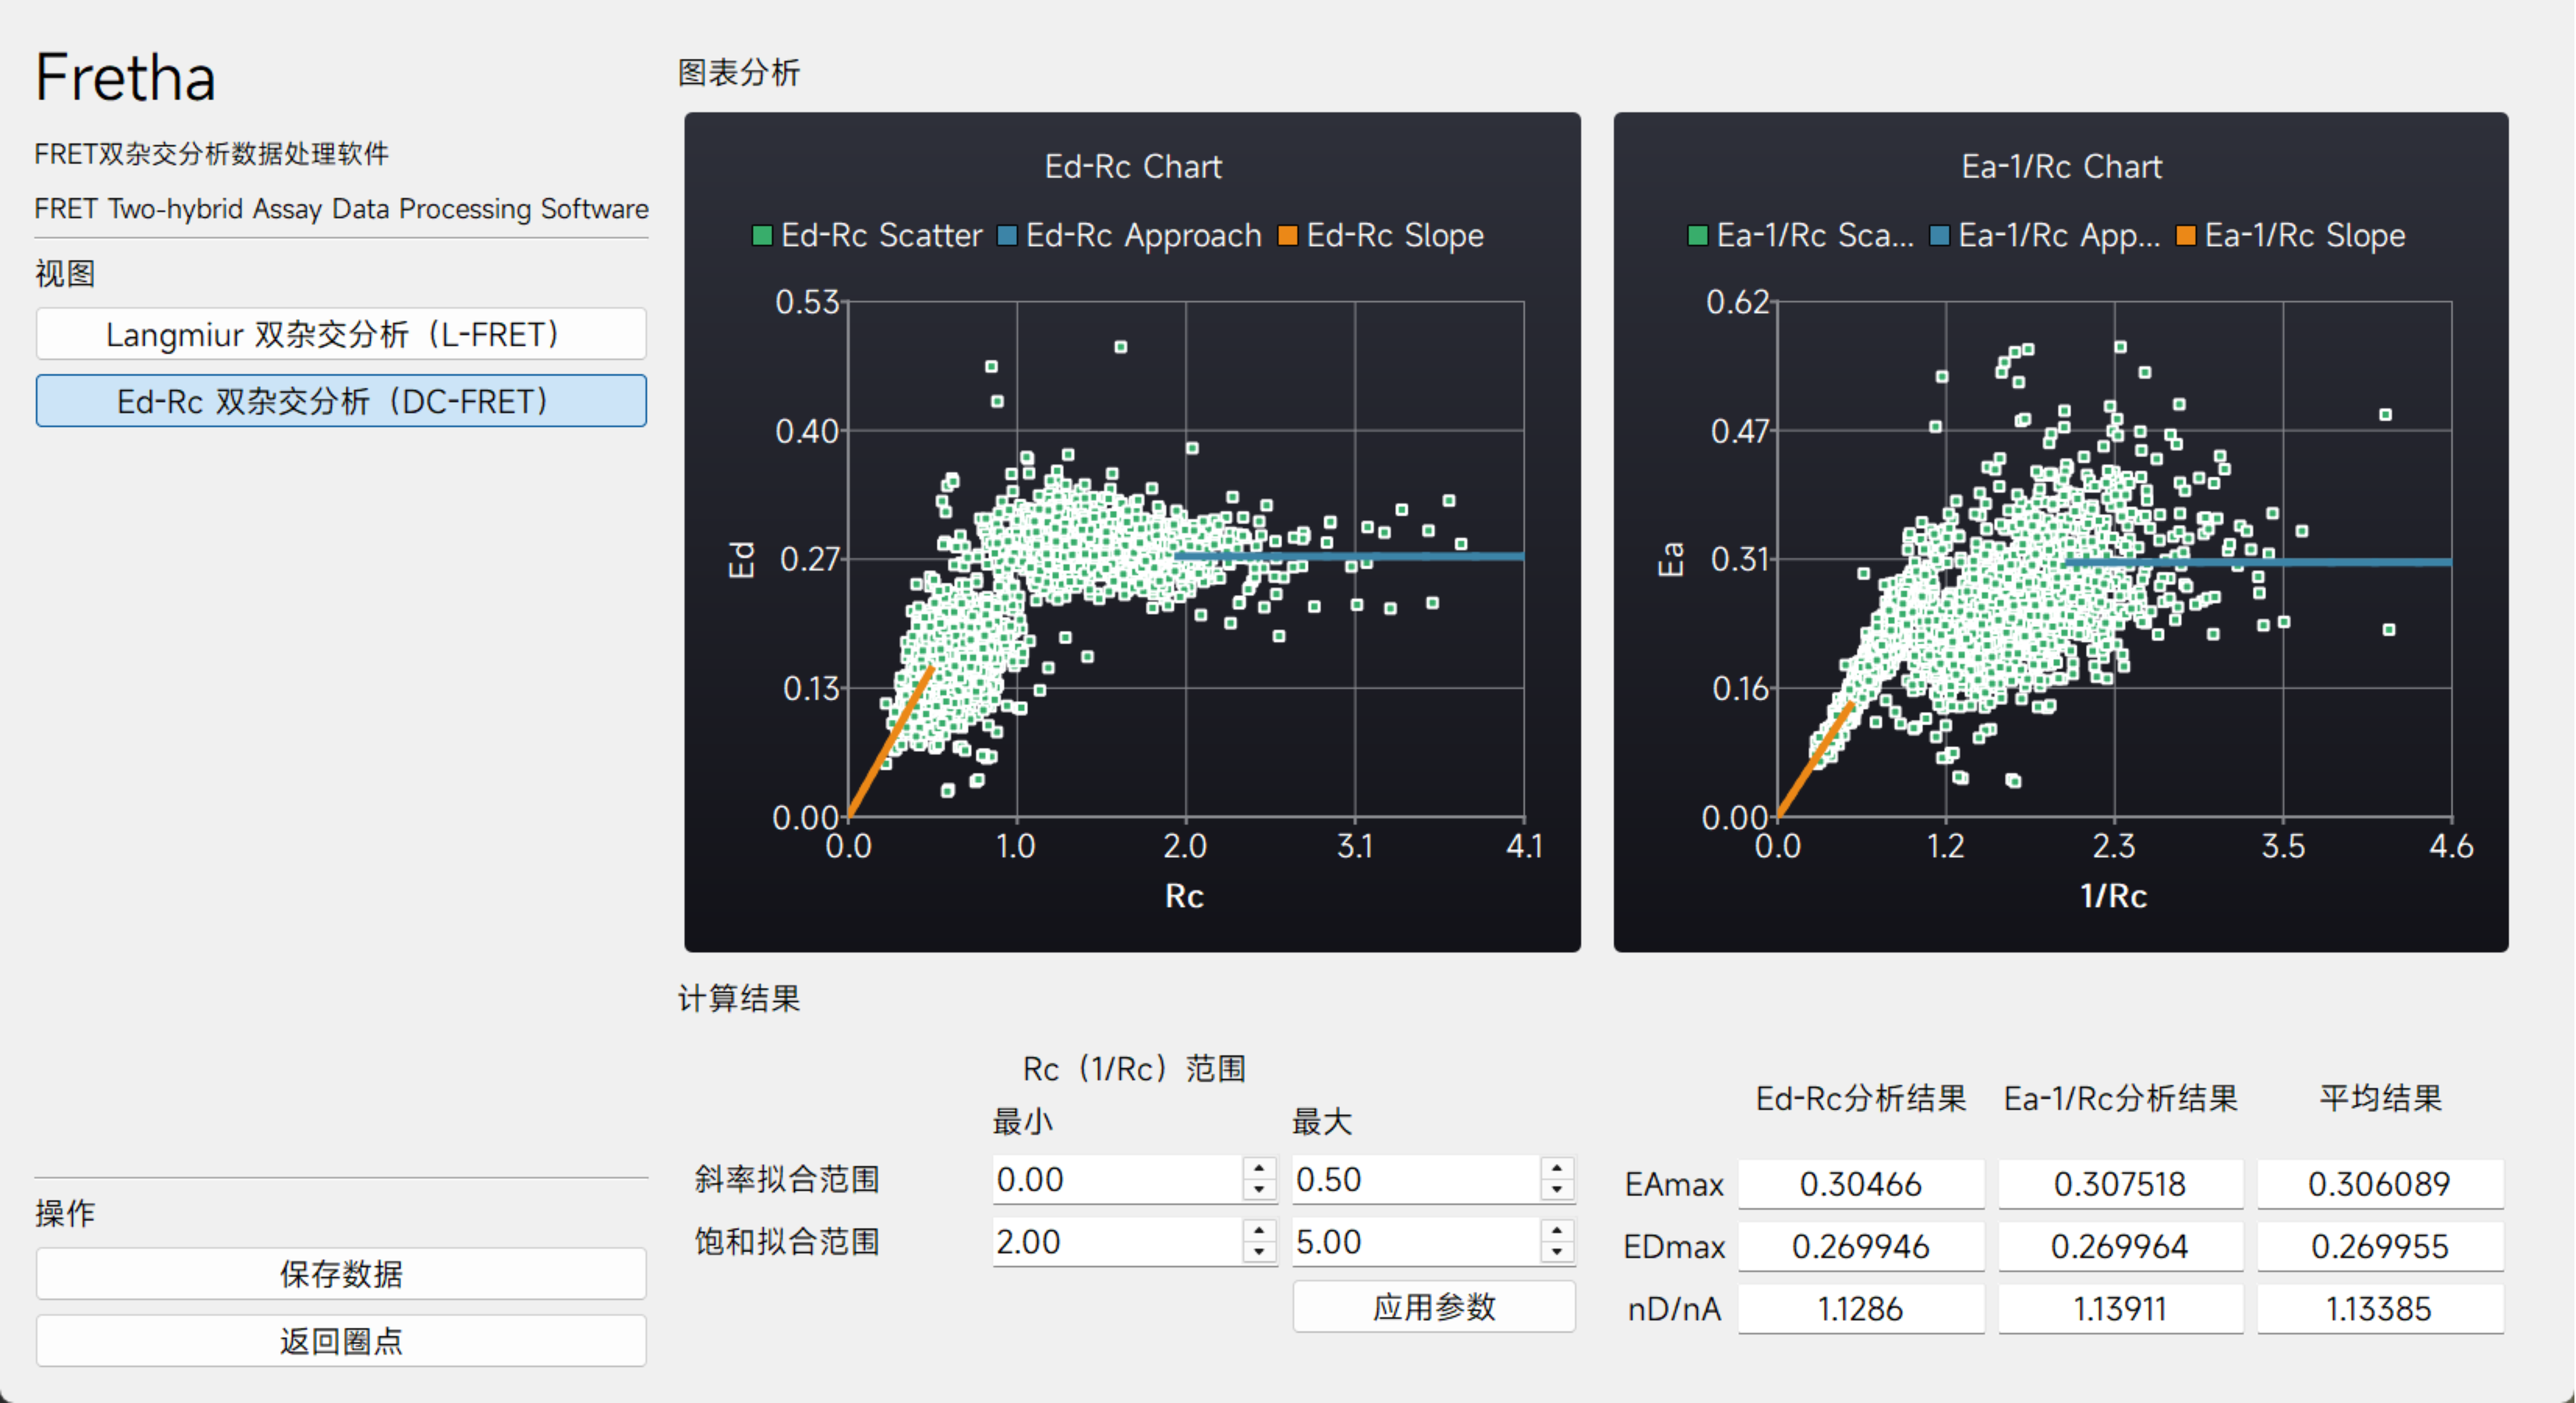
\includegraphics[width=0.9\linewidth]{../figures/2/2_DC-FRET结果界面.png}
  \caption{Fretha DC-FRET视图}
  \label{fig:fretha_dc_fret}
\end{figure}

DC-FRET视图的界面如图 \ref{fig:fretha_dc_fret} 所示。
在DC-FRET视图模式下,软件能显示出DC-FRET的拟合结果,包括$E_{A,max}$、$E_{D,max}$、$n_D/n_A$,以及拟合曲线和实验数据的对比图。
界面中设计了调整线性拟合参数的设置栏,用户可以调整$R_C$($1/R_C$)的数据范围,点击“更新”按钮以应用范围参数,用来处理复杂的数据。

点击“保存结果”按钮后,系统将同步存储拟合结果数据、可视化图像及实验数据,保存结果如图表所示。
\begin{table}[htbp]
  \centering
  \caption{结果保存生成文件}
  \label{tab:fretha_result_list}
    \begin{tabular}{cc}
      \toprule[1.5pt]
      {文件名} & {说明} \\
      \midrule
      Ea-Rda图.png & $E_A$-$1/R_C$散点和趋势线图 \\
      Ed-Rad图.png & $E_D$-$R_C$散点和趋势线图 \\
      Ea-Dfree图.png & $E_A$-$D_{free}$散点和趋势线图 \\
      Ed-Afree图.png & $E_D$-$A_{free}$散点和趋势线图 \\
      FretThaData.csv & FRET双杂交分析结果数据 \\
      FretThaResults.csv & FRET双杂交分析结果拟合参数 \\
      \bottomrule[1.5pt]
    \end{tabular}
\end{table}
其中,实验数据与拟合参数的原始数值将以 CSV 文件格式进行保存,该文件包含可直接用于其他科研绘图软件的数据记录,从而支持用户在不同可视化工具中进行后续的图形优化与再处理。
这一功能设计保障了实验结果的完整留存,为科研工作者提供了灵活的数据导出与再分析解决方案。
\fi

\section{本章小结}
本章系统阐述了 FRET 双杂交分析数据处理软件 Fretha 的设计框架与实现方法。
通过采用分层架构,Fretha采用了表现层、业务层、数据访问层和数据层的四层架构体系(图 \ref {fig:fretha_arch}),从而实现了软件的解耦设计。
基于 FRETScope 显微成像系统的多模态数据特征,数据层采用 FretImage-FretDataPiece-FretRecord 三级关联模型(图 \ref {fig:fretha_data_relations}),实现了从原始图像到分析结果的全流程数据管理。
按照FRET双杂交数据处理步骤流程,将软件的功能划分为成像参数设置、数据检验、FRET图像处理、数据管理和结果可视化五个功能模块。
基于OpenCV和Dlib等开源计算库,本章构建了包含 FRET 定量计算器、图像处理器和双杂交求解器的后台接口,实现了 E-FRET、 $3^3$-FRET、DC-FRET、L-FRET等多模态FRET算法。
在 L-FRET 分析中,采用基于 BFGS 算法的非线性优化策略(代码 \ref {code:two_hybrid_solver}),完成 Langmuir 模型的参数拟合。
基于分层架构设计和功能模块化设计,本章实现了每个功能模块,支持了FRET双杂交分析的复杂数据处理功能,
最终开发实现了一款拥有用户友好界面、简单易用、处理高效的FRET双杂交分析专业数据处理软件。
\chapter{自动FRET双杂交分析}

\section{引言}

\ifshowtext
FRET双杂交分析在生物研究中作用重大,却面临两大难题。一是数据处理复杂又耗时,涵盖选 ROIs、定荧光强度与背景、估算 FRET 效率和拟合曲线等约 50 个关键步骤,每次实验处理需 5 - 6 小时。二是对数据质量要求很高,要尽量减少异常值,否则会影响朗缪尔模型拟合,导致结果偏差。
当前 FRET 技术提取荧光强度主要靠有监督的机器学习方法,像 U - Net 模型和 ilastik 工具。但这些算法依赖人工标注数据集,效果受其大小和质量影响,且可解释性差,神经网络模型难以提供清晰数学框架解释分析模式。
针对这些问题,本文提出基于亮度均匀性的 ROI 选择(LURS)算法用于荧光数据提取。该算法受到人工处理数据时重要的明度(Luminance)和均匀度(Uniformity)启发,利用局部标准差排除灰度突变区域,提升数据提取质量。
在 C32V 和 CVC 质粒上验证了精度。本方法准确性与人工处理相当,速度更快,提升了 FRET 双杂交分析在高通量筛选中的实用性。
\fi

\section{材料与方法}

\ifshowtext
\fi

\subsection{细胞培养和转染}
\label{sec:细胞转染}
\ifshowtext
用于标准质粒实验的MCF-7细胞系购自中国科学院细胞库,培养于含有10\%胎牛血清(FBS)、100 U/ml青霉素和100 μg/ml链霉素的DMEM培养基中。对于药物作用实验,将MCF-7细胞以每孔4000细胞的密度接种于96孔板(LABSELECT,中国)中,加入DMEM和10\% FBS,置于37$^\circ \text{C}$、5\% CO2的孵箱中培养12小时。每孔转染400 ng的质粒,使用3:1或1:3比例的转染复合物进行转染。
\fi

\subsection{FRET成像系统}
\label{sec:成像条件}
\ifshowtext
本研究中,所有实验数据均使用自主研发的多模态FRET自动化成像系统获取 \upcite{sun2022automated}。
对于CY标准质粒,实验选用了20倍的0.45NA物镜(Olympus,日本)和6\%光照强度。
模型质粒实验,选用了20倍的0.45NA物镜(Olympus,日本)和50\%光照强度。
实验过程中,在AA通道寻找视野,然后依次捕获AA、DA和DD通道的荧光图像。

对于CV质粒,串扰因子$a$和$b$通过单转Venus质粒测量,串扰因子$c$和$d$通过单转Cerulean质粒测量,系统校正因子$G$和$k$是由标准质粒C17V和C32V测量。

对于CY质粒,串扰因子$a$和$b$通过单转YFP质粒测量,串扰因子$c$和$d$CFP质粒测量,系统校正因子$G$和$k$是由标准质粒C4Y、C10Y、C40Y和C80Y质粒测量。
所有的FRET成像参数如表\ref{tab:lurs_imaging_params}所示。

\begin{table}[htbp]
    \centering
    \caption{FRET成像系统参数}
    \begin{tabularx}{\linewidth}{>{\centering\arraybackslash}X>{\centering\arraybackslash}X>{\centering\arraybackslash}X}
        \toprule
        参数名 & CV质粒成像参数 & CY质粒成像参数 \\
        \midrule
        a & 0.206 & 0.160\\
        b & 0.040 & 0.002\\
        c & 0.047 & 0.003\\
        d & 0.789 & 0.784\\
        G & 4.224 & 6.430\\
        k & 0.635 & 0.406\\
        $\varepsilon_{YFP}(\lambda)/\varepsilon_{CFP}(\lambda)$ & 0.077 & 0.064\\
        \bottomrule
    \end{tabularx}
    \label{tab:lurs_imaging_params}
\end{table}
\fi

\subsection{基于明度和均匀度的自动ROI选取算法(LURS)}
不失一般性,我们将ROI定义为$n \times n$的正方形区域,这种设计简化了标注过程并增强了基于积分的图像优化方法的适用性,从而显著提升计算效率\upcite{jagadeeswari2022integral}。参数$n$与细胞的像素面积相关,本文实验中在20倍放大条件下设定为5。

LURS算法包含以下步骤:

\begin{enumerate}
\item \textbf{图像预处理。}  
对FRET三通道图像的预处理主要包括原始图像的平滑处理和背景灰度值的扣除。从三个通道采集的原始图像分别记为$I_{Raw,DD}$、$I_{Raw,DA}$和$I_{Raw,AA}$。为了获得更精确的定量分析结果,我们采用高斯模糊对图像进行平滑处理,利用钟形曲线为像素分配权重影响\upcite{gedraite2011investigation}。  
背景强度($I_{BG}$)通过识别直方图中出现频率最高的像素值确定,因为图像中大部分像素属于背景且灰度值集中\upcite{sun2019}:
\begin{equation}
    I_{BG} = \underset{p}{\arg\max} H(p), 
    \label{eq:bg}
\end{equation}
其中$p$遍历所有可能的像素值,$\underset{p}{\arg\max} H(p)$表示使$H(p)$达到最大值的像素值$p$,该值即为计算得到的背景强度$I_{BG}$。处理后的图像重新命名为$I_{DD}$、$I_{DA}$和$I_{AA}$,准备进行后续处理。

\item \textbf{基于亮度的自适应阈值分割。}  
在荧光成像中,避免低亮度区域(如细胞空腔)对于获取高质量荧光信号至关重要。传统单阈值方法可能错误排除低亮度细胞并误判不应参与荧光分析的明亮空腔。我们采用局部自适应阈值方法对平滑后的图像($I_{DD}$、$I_{DA}$和$I_{AA}$)进行二值化分割。像素$(x, y)$的阈值$T_L(x,y)$和二值化结果${Mask}_L(x,y)$计算如下:
\begin{equation}
    T_L(x,y)=\frac{1}{w \times w} \sum_{i=x-\frac{w-1}{2}}^{x+\frac{w-1}{2}} \sum_{j=y-\frac{w-1}{2}}^{y+\frac{w-1}{2}} I(i,j)+b_L,
    \label{eq1}
\end{equation}
\begin{equation}
    {Mask}_L(x,y)=\begin{cases}
        1,&I(x,y) \geq T_L(x,y) \\
        0,&I(x,y) < T_L(x,y)
    \end{cases},
    \label{eq2}
\end{equation}
其中$I(x,y)$为输入图像的灰度值,$w$为大于等于$4n+1$但不超过细胞长宽四分之一的奇数,$b_L$为偏置项(设置为各视图通过式(\ref{eq:bg})计算的背景灰度值),确保完全去除背景区域。

\item \textbf{三通道掩码合并生成${Mask}_L$。}  
三通道图像的掩码通过逻辑与操作合并生成最终掩码:
\begin{equation}
    \begin{split}
    {Mask}_L(x,y)={Mask}_{L,DD}(x,y) \land {Mask}_{L,DA}(x,y) \land {Mask}_{L,AA}(x,y),
    \end{split}
    \label{eq3}
\end{equation}
其中${Mask}_{L,DD}$、${Mask}_{L,DA}$和${Mask}_{L,AA}$是基于式(\ref{eq2})生成的各通道掩码,${Mask}_{L}$为合并结果。

\item \textbf{计算ROI的CV矩阵。}  
均匀性反映特定区域内荧光信号的一致性,对保证实验数据的可靠性和可重复性具有重要意义。我们采用变异系数(CV)评估ROI内的灰度均匀性:
\begin{equation}
   {CV}_{ROI}={StdDev}_{ROI} / {Mean}_{ROI},
    \label{eq4}
\end{equation}
其中${Mean}_{ROI}$为ROI内像素的平均灰度值,${StdDev}_{ROI}$为标准差。我们计算每个ROI的CV值并存储为$CV$矩阵(${Mat}_{CV}$)。  
同时生成均值矩阵${Mat}_{Mean}$存储各ROI的均值,像素$(x,y)$的值计算为:
\begin{equation}    
    {Mat}_{Mean}(x,y)=\frac{1}{n \times n} \sum_{i=x- \frac{n-1}{2}}^{x+\frac{n-1}{2}} \sum_{j=y-\frac{n-1}{2}}^{y+\frac{n-1}{2}} I(i,j),
    \label{eq5}
\end{equation}
其中$n$为ROI宽度。基于均值矩阵,标准差矩阵计算为:
\begin{equation}
    \begin{split}
    {Mat}_{Std}(x,y)=
    \sqrt{\frac{1}{n \times n} \sum_{i=x-\frac{n-1}{2}}^{x+\frac{n-1}{2}} \sum_{j=y-\frac{n-1}{2}}^{y+\frac{n-1}{2}}{I(i,j)}^2-{{Mat}_{Mean}(x,y)}^2},
    \end{split}
    \label{eq6}
\end{equation}
将各ROI的CV值存入${Mat}_{CV}$:
\begin{equation}
    {Mat}_{CV}={Mat}_{Std}(x,y)/{Mat}_{Mean}(x,y),
    \label{eq7}
\end{equation}
并通过线性变换将浮点型CV值转换为16位整数:
\begin{equation}
    {I}_{CV}(x,y)=\left\lfloor\frac{{Mat}_{Std}(x,y)-{Std}_{min}} {{Std}_{max}-{Std}_{min}}\times65535 + 0.5\right\rfloor,
\end{equation}
其中${Std}_{min}$和${Std}_{max}$为${Mat}_{CV}$的最小和最大CV值,$I_{CV}$为转换后的0-65535范围的整数值。

\item \textbf{基于均匀性的自适应阈值分割CV矩阵。}  
三通道CV矩阵记为$I_{CV,DD}$、$I_{CV,DA}$和$I_{CV,AA}$。采用与生成${Mask}_{L}$相同的方法生成基于均匀性的掩码(注意低CV值区域更优)。像素$(x,y)$的阈值计算为:
\begin{equation}
    T_U(x,y)=\frac{1}{w \times w} \sum_{i=x-\frac{w-1}{2}}^{x+\frac{w-1}{2}} \sum_{j=y-\frac{w-1}{2}}^{y+\frac{w-1}{2}} {I}_{CV}(i,j)+b_U,
    \label{eq8}
\end{equation}
\begin{equation}
    {Mask}_U(x,y)=\begin{cases}1,&I(x,y) < T_U(x,y)\\ 0,&I(x,y) \ge T_U(x,y)\end{cases},
    \label{eq9}
\end{equation}
其中$b_U$通过式(\ref{eq:bg})对$I_{CV}(x,y)$计算得到。

\item \textbf{三通道均匀性掩码合并生成${Mask}_U$。}  
\begin{equation}
    \begin{split}
    {Mask}_{U}(x,y)={Mask}_{U,DD}(x,y) \land {Mask}_{U,DA}(x,y) \land {Mask}_{U,AA}(x,y),
    \end{split}
    \label{eq_merge_u}
\end{equation}
其中${Mask}_{U,DD}$、${Mask}_{U,DA}$和${Mask}_{U,AA}$是基于式(\ref{eq9})生成的各通道均匀性掩码,${Mask}_{U}$为合并结果。

\item \textbf{合并亮度掩码与均匀性掩码生成${Mask}_{LU}$。}  
通过逻辑与操作合并亮度掩码和均匀性掩码:
\begin{equation}
    {Mask}_{LU}(x,y)={Mask}_L(x,y) \land {Mask}_U(x,y)
    \label{eq10}
\end{equation}

\item \textbf{从${Mask}_{LU}$中选择ROI。}  
对掩码进行连通区域分析,移除面积小于$n \times n$的碎片区域。选择高信噪比像素作为ROI中心,通过${Mat}_{Mean}$获取对应位置的信号值。
\end{enumerate}

LURS算法流程如图\ref{fig1}所示:

\begin{figure*}[!htbp]
\centering
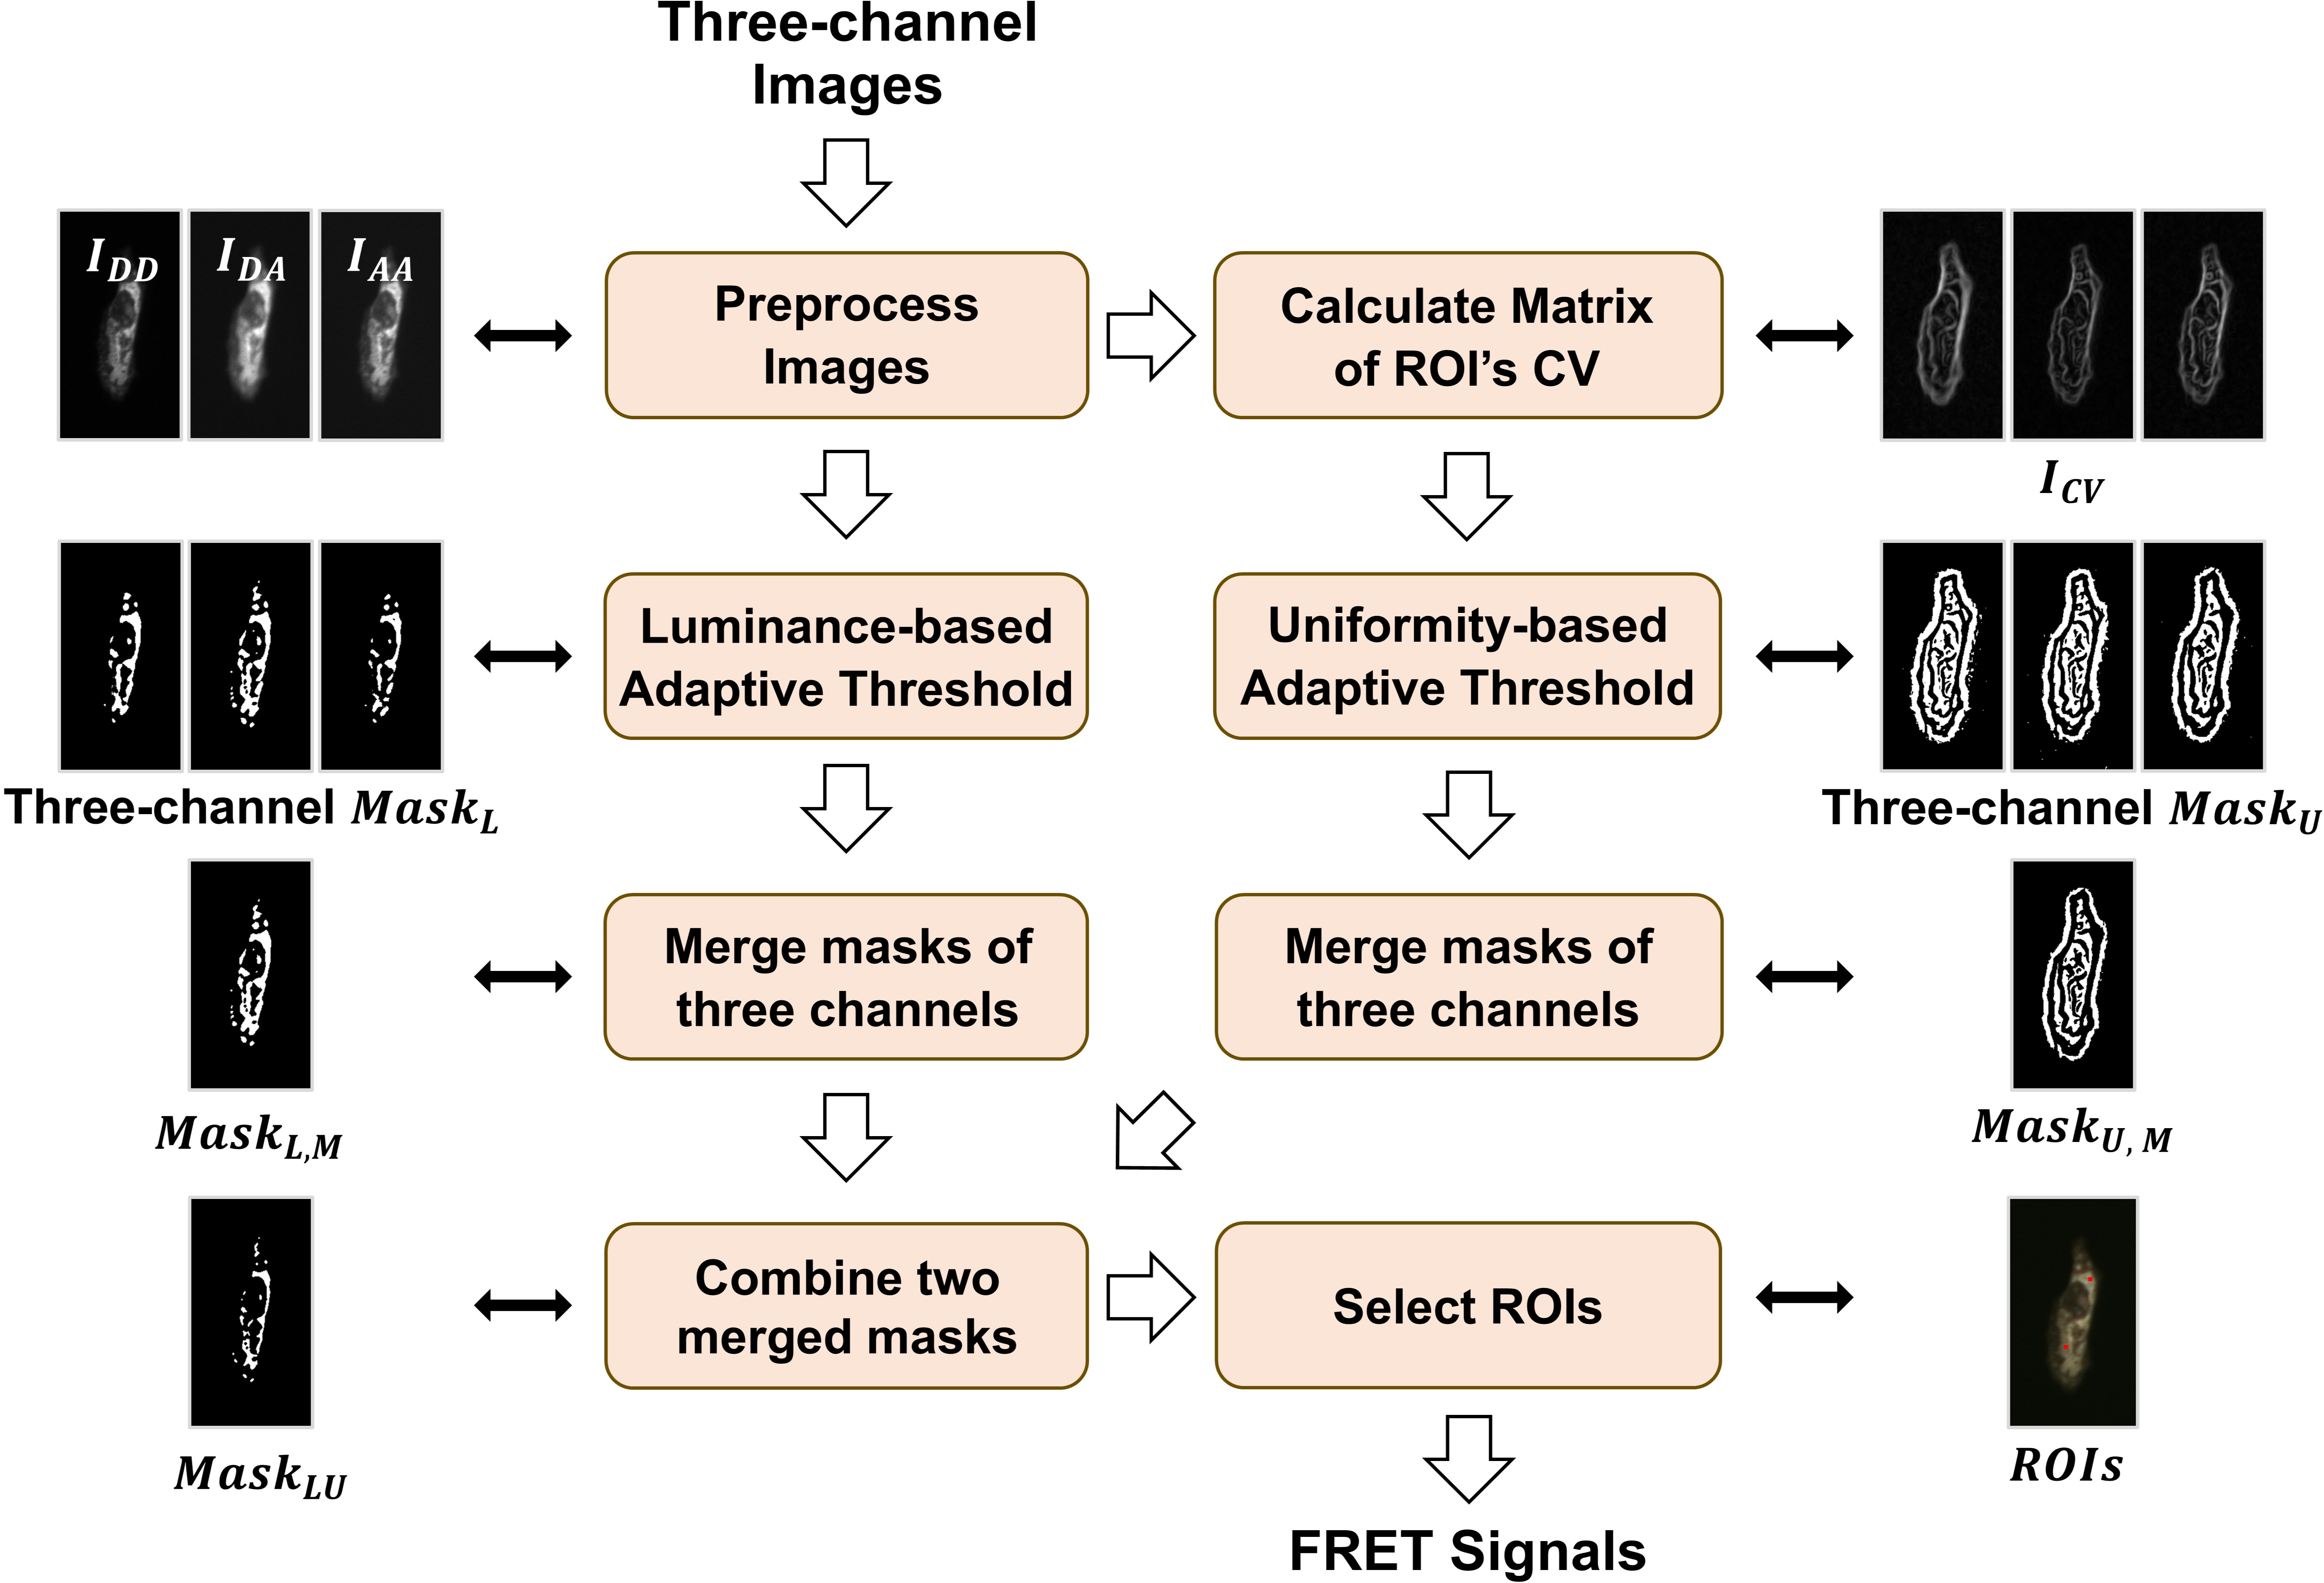
\includegraphics[width=1\linewidth]{../figures/3/3_LURS流程图.png}
\caption{LURS算法流程图}\label{fig1}
\end{figure*}

\subsection{DC-FRET方法的数据范围选取}
\ifshowtext
在自动FRET双杂交分析数据处理中,我们更倾向于使用DC-FRET方法而L-FRET方法,因为DC-FRET方法具有以下优势:
\begin{enumerate}
    \item \textbf{简化实验过程:}与L-FRET方法相比,DC-FRET方法无需在中间分布状态下准备大量样本。相反,仅需准备相对较大$R_C$值和相对较小$R_C$值的样本,这减少了样本的制备和处理时间。
    \item \textbf{得出更稳定可靠的结果:}DC-FRET中用于线性拟合的供体荧光能量转移效率($E_D$)和$R_C$数据是通过E-FRET方法进行定量测量的,该方法具有较高的准确性和稳定性,能够提供可靠的数据,使得线性拟合的结果更加稳定可靠。
\end{enumerate}

然而,DC-FRET方法在选择$R_C$或$1/R_C$的范围时需要一定经验。如果所选范围过小,将会导致数据点不足,从而使结果的稳定性变差。当拟合范围过大时,结果可能会不正确,因为这可能不符合相关原理的条件。为了避免使用数据中的不稳定部分,我们总结以下原则,以实现自动的DC-FRET分析:
\begin{enumerate}
    \item 如果样本仅包含供体饱和的情况或仅包含受体饱和的情况,应选择$R_C$($1/R_C$)值相对较小的50\%的数据。
    \item 当受体饱和和供体饱和同时存在时,则应选择$R_C$($1/R_C$)值较小的25\%的数据。
\end{enumerate}

\fi

\section{实验结果}

\subsection{标准质粒验证实验}
准确获取正确且可靠的$3^3$-FRET和 E-FRET的计算结果,是成功进行FRET双杂交分析的必要前提。
因此,我们运用我们的方法对青色荧光蛋白(CFP)和黄色荧光蛋白(YFP)构建体的单质粒进行了测量,具体包括 C4Y、C10Y、C40Y 和 C80Y。相应的结果列于表\ref{tab:results_standard_plasmids}中。

\begin{table*}[htbp]
    \centering
    \caption{ 对标准质粒进行$3^3$-FRET和E-FRET测量的结果}
    \begin{tabularx}{\linewidth}{
    >{\centering\arraybackslash}X
    >{\centering\arraybackslash}X
    >{\centering\arraybackslash}X
    >{\centering\arraybackslash}X
    >{\centering\arraybackslash}X
    >{\centering\arraybackslash}X
    >{\centering\arraybackslash}X}
    \toprule
    \multirow{2}{*}{样本} & \multicolumn{3}{c}{测量结果} & \multicolumn{3}{c}{文献结果} \\
     & $E_{A}$ & $E_{D}$ & ${R_C}$ & $E_A$ & $E_{D}$ & $R_C$ \\
    \midrule
    C4Y  & $0.31\pm0.04$ & $0.29\pm0.02$ & $0.98\pm0.11$ & $0.30$ & $0.30$ & $1$ \\
    C10Y & $0.24\pm0.02$ & $0.21\pm0.02$ & $0.94\pm0.10$ & $0.22$ & $0.23$ & $1$ \\
    C40Y & $0.17\pm0.03$ & $0.15\pm0.01$ & $0.98\pm0.17$ & $0.16$ & $0.16$ & $1$ \\
    C80Y & $0.11\pm0.03$ & $0.11\pm0.02$ & $1.03\pm0.20$ & $0.12$ & $0.12$ & $1$ \\
    \bottomrule
    \end{tabularx}
    \label{tab:results_standard_plasmids}
\end{table*}

通过对LURS 提取的ROI的FRET信号进行计算和统计分析,结果表明:C4Y 的$E_D$值为 0.31,C10Y 的$E_D$为 0.23,C40Y 的$E_D$为 0.2,C80Y 的$E_D$为 0.11。
与此同时,C4Y、C10Y、C40Y 和 C80Y 的$R_C$值分别为 0.98、0.94、0.98 和 1.03,与标准值1接近。
所有质粒的$E_D$和$R_C$值都与已报道的值接近,这表明 LURS 算法能够成功提取出正确且有效的ROI,为FRET双杂交分析提供了从供体和受体角度的准确FRET效率数据。

\subsection{模型质粒验证实验}

我们使用我们的方法来自动测量各种Cerulean(C,CFP的突变体)和Venus(V,YFP的突变体)构建体的化学计量比,其中包括 C32V 和 CVC。图\ref{fig:results_model_plasmids}展示了共表达 C32V / CVC 且含有游离的 C(C32V + C,CVC + C)(上半部分)或游离的 V(C32V + V,CVC + V)(下半部分)的活 MCF7 细胞的三张荧光图像(DD、AA 和 DA)(左侧),以及由 LURS 生成的ROI(中间),还有图和图(右侧)。

\begin{figure}[htbp]
    \centering
    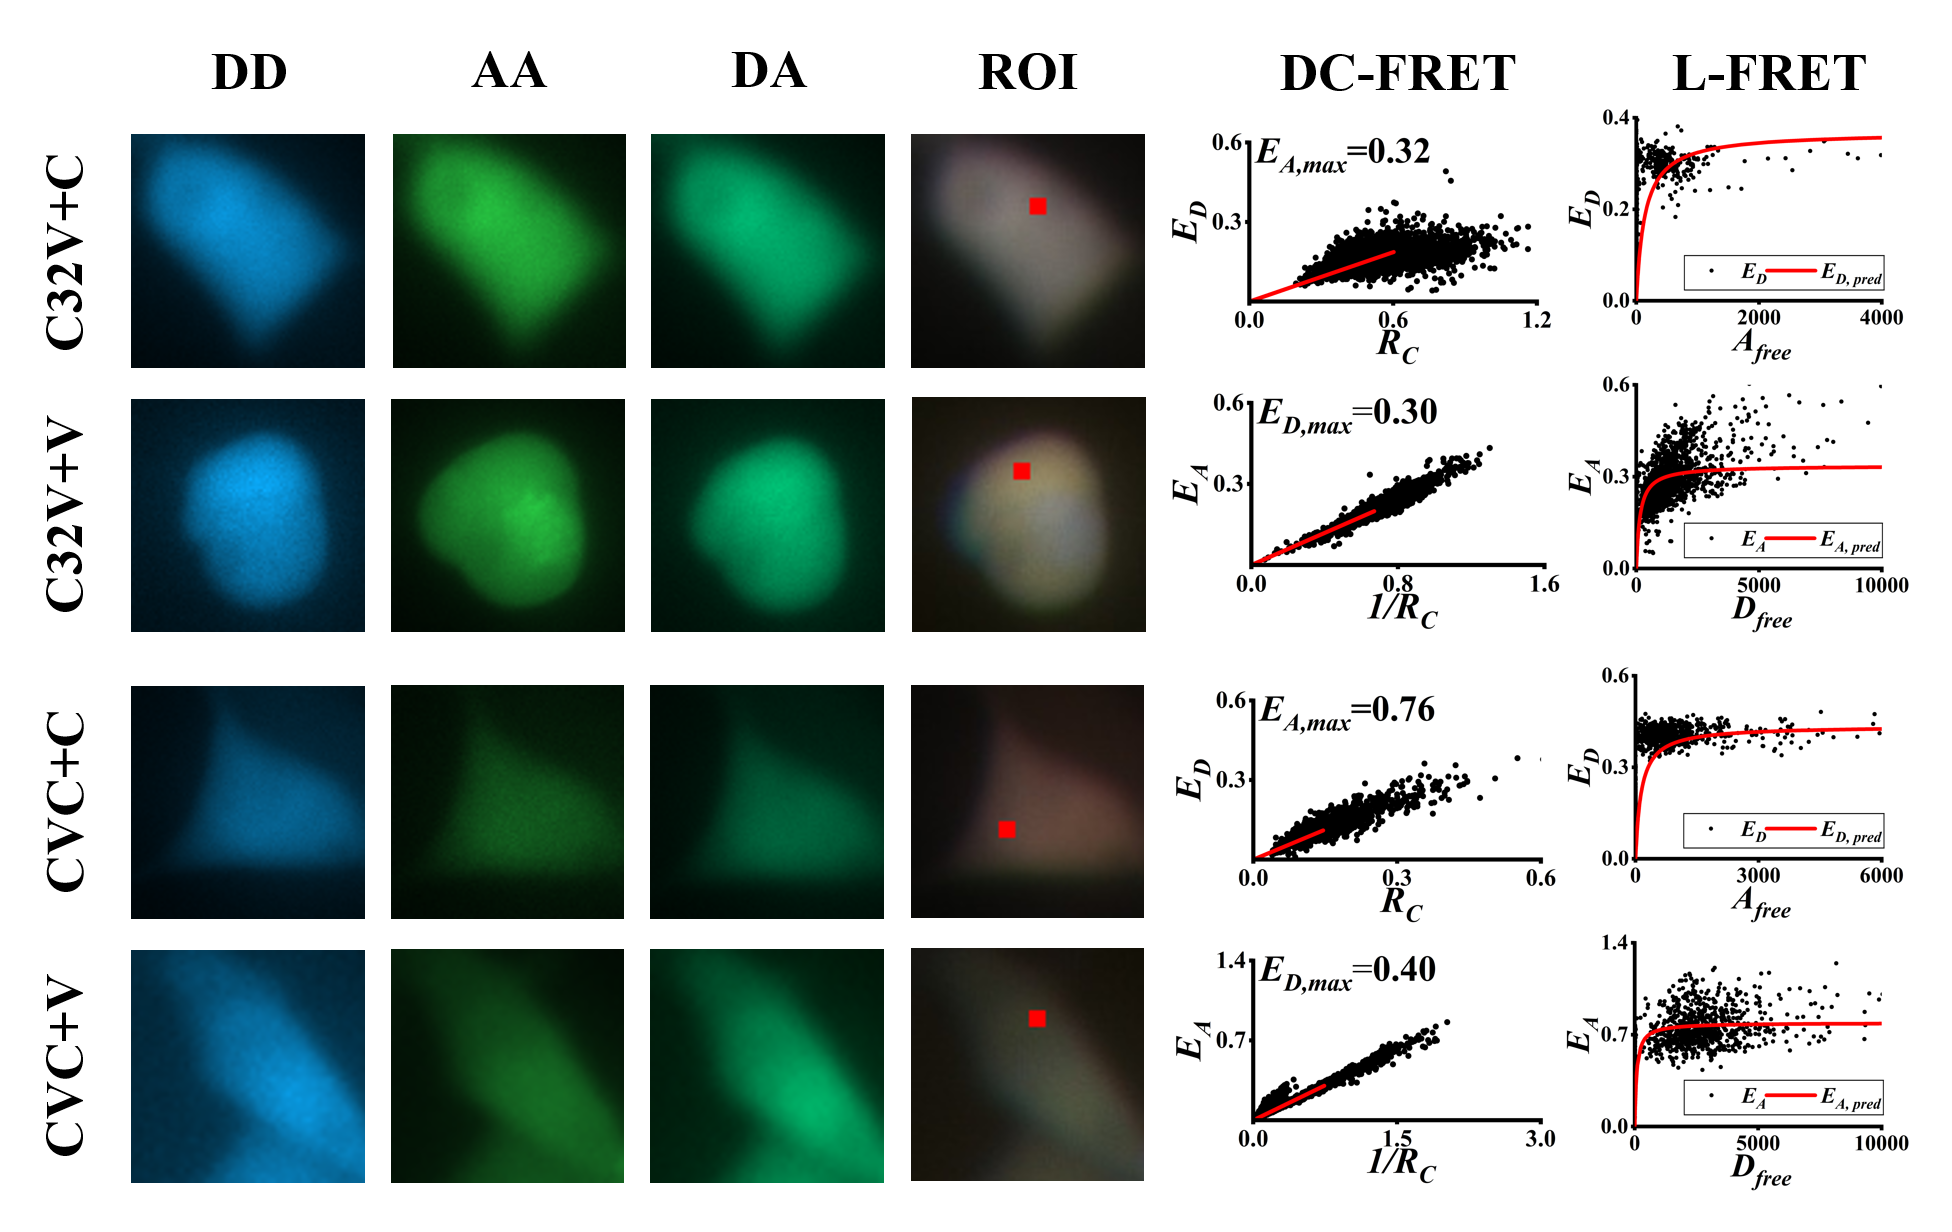
\includegraphics[width=1\linewidth]{../figures/3/3_模型质粒实验结果.png}
    \caption[模型质粒验证实验结果]{在存在游离供体或受体的情况下,分别通过DC-FRET和L-FRET方法对MCF7活细胞中标准质粒(C32V和CVC)的$E_{A, max}$、$E_{D, max}$和$n_D/n_A$进行自动FRET双杂交分析测量结果。}
    \label{fig:results_model_plasmids}
\end{figure}

运用相同的方法,我们测量了 C32V 和 CVC 质粒中Cerulean与Venus之间的结合化学计量比,测量结果见表\ref{tab:results_model_plasmids}。
对于 C32V 质粒,我们得到的$E_{A,max}$为 0.32,$E_{D,max}$为 0.30,化学计量比($n_D/n_A$)为 1.06。
这个数值与 C32V 预期的供体-受体比例 1:1非常接近。
对于 CVC 质粒,$E_{A,max}$、$E_{D,max}$和$n_D/n_A$的值分别为 0.76、0.40 和 1.90,所获得的结果与先前文献中报道的结果一致\upcite{koushik2006cerulean}。
对于这两种化学计量比不同的质粒,我们的方法成功识别到了它们的化学计量比的差别,且计算出的化学计量比的相对误差不超过 6\%,进一步证明了我们方法的准确性。

\begin{table*}[htbp]
    \centering
    \caption{模型质粒的FRET双杂交分析结果}
    \begin{tabularx}{\linewidth}{
    >{\centering\arraybackslash}X
    >{\centering\arraybackslash}X
    >{\centering\arraybackslash}X
    >{\centering\arraybackslash}X
    >{\centering\arraybackslash}X
    >{\centering\arraybackslash}X}
    \toprule
    \multirow{2}{*}{样本} & \multicolumn{3}{c}{测量结果} & \multicolumn{2}{c}{文献结果} \\
     & $E_{A,max}$ & $E_{D,max}$ & ${n_D/n_A}$ & $E_{D,max}$ & $n_D/n_A$\\
    \midrule
    C32V & $0.32\pm0.04$ & $0.30\pm0.01$ & $1.06\pm0.14$ & 0.31 & 1\\
    CVC & $0.76\pm0.02$ & $0.40\pm0.02$ & $1.90\pm0.11$ & 0.41 & 2\\
    \bottomrule
    \end{tabularx}
    \label{tab:results_model_plasmids}
\end{table*}

\section{本章小结}

\ifshowtext
本章针对传统 FRET 双杂交分析中数据处理效率低、质量依赖人工标注等问题,提出基于亮度均匀性的 ROI 选择算法(LURS)。该算法通过高斯平滑预处理、多通道自适应阈值分割和变异系数均匀性评估,实现了荧光信号的高效提取。实验结果表明,LURS 算法在标准质粒 C4Y/C10Y/C40Y/C80Y 的 E-FRET 测量中,EA 与 ED 值与文献报道误差小于 5\%,RC 值偏差不超过 0.05,验证了算法的准确性。在模型质粒 C32V 和 CVC 的化学计量比分析中,测量的 nD/nA 值分别为 1.06±0.14 和 1.90±0.11,与理论值 1:1 和 2:1 高度吻合,且计算效率较人工处理提升 80\% 以上。结合 DC-FRET 方法的自动数据范围选取策略,该系统成功实现了 FRET 双杂交分析的全流程自动化,为高通量药物筛选和蛋白质互作研究提供了可靠的技术支撑,丰富了数据处理软件Fretha的功能。
\fi
\chapter{Fretha的测试}

\section{引言}
\ifshowtext

本章我们应用我们开发的FRET双杂交分析数据处理软件,分析Bcl-xL和Bak互作时加入Bcl-xL抑制剂A1331852前后的互作变化情况\upcite {2020Stoichiometry}。
针对自动数据处理算法,我们对比了基于深度学习的自动数据处理方法,包括交互式医学图像分析软件ilastik和面向2D医学图像特化的分割大模型SAM\_Med2D,结果发现,计算结果也更接近手动处理的数据结果,速度最优,系统硬件配置要求也最低。
最后,在数据处理过程中,我们对软件的稳定性和功能进行验证,结果表明,Fretha软件运行稳定,所有功能符合预期。

\fi

\section{Fretha功能测试}
软件测试是确保软件质量和性能的重要环节。结合Fretha的应用实验,我们对软件的功能模块进行了测试,包括成像参数设置、数据导入导出、结果保存、软件性能和稳定性等方面。测试结果表明,Fretha软件在大部分情况下能够正常工作,但在一些极端情况下可能会出现问题,需要进一步优化和改进。

\subsection{成像参数设置模块测试}
成像参数设置是软件的核心功能之一,直接影响到数据处理结果的准确性。本测试旨在验证软件成像参数设置功能的正确性和灵活性,确保软件能够及时准确响应参数的更新设置。

在测试方法上,本节通过界面操作更新参数,分别用CV成像参数和CY参数处理单转标准质粒C32V和C4Y样本的FRET图像数据,将数据导出后,检查E-FRET计算结果$E_D$和$R_C$。具体测试步骤如下:
\begin{enumerate}
    \item 打开软件,进入成像参数设置界面。
    \item 使用表 \ref{tab:lurs_imaging_params} 中CV质粒成像的参数进行设置,然后处理单独转染C32V质粒样本数据和单独转染C4Y质粒样本数据。
    \item 退出参数设置界面,再次进入参数设置界面。
    \item 使用表 \ref{tab:lurs_imaging_params} 中CY质粒成像的参数进行设置,然后处理单独转染C32V质粒样本数据和单独转染C4Y质粒样本数据。
    \item 关闭软件,重新打开软件,然后进入参数设置界面。
    \item 记录两次数据处理的结果。
\end{enumerate}

\begin{table*}[htbp]
    \centering
    \caption{ 切换参数对C32V质粒和C4Y质粒的E-FRET分析结果}
    \begin{tabularx}{\linewidth}{
    >{\centering\arraybackslash}X
    >{\centering\arraybackslash}X
    >{\centering\arraybackslash}X
    >{\centering\arraybackslash}X
    >{\centering\arraybackslash}X
    >{\centering\arraybackslash}X
    >{\centering\arraybackslash}X}
    \toprule
    \multirow{2}{*}{参数} & \multicolumn{2}{c}{C32V} & \multicolumn{2}{c}{C4Y} \\
    & $E_{D}$ & ${R_C}$ & $E_{D}$ & $R_C$ \\
    \midrule
    CV体系参数 & $0.29\pm0.02$ & $0.98\pm0.11$ & $0.22\pm0.03$ & $1.31\pm0.13$  \\
    CY体系参数 & $0.38\pm0.05$ & $0.82\pm0.09$ & $0.30\pm0.02$ & $1.02\pm0.12$  \\
    \bottomrule
    \end{tabularx}
    \label{表:测试参数更新}
\end{table*}

从软件界面上,在设置参数后重新进入参数设置界面,发现参数符合预期的新参数。在软件重启后,发现界面显示的参数也与最近一次更新的参数一致。
说明软件界面能够准确显示最新的参数设置。

两次E-FRET分析的结果如表 \ref{表:测试参数更新} 所示。在计算功能上,在更新了CY成像参数后,处理C32V质粒计算得到的$E_D$和$R_C$结果分别为0.38和0.82,处理C4Y质粒,计算得到的$E_D$和$R_C$结果分别为0.30和1.02;
在使用CV参数处理C4Y质粒时,计算得到的$E_D$和$R_C$结果分别为0.22和1.31,处理C32V质粒时,计算得到的$E_D$和$R_C$结果分别为0.29和0.98。文献报道的C4Y质粒和C32V质粒的$E_D$为0.30,$R_C$结果为1。可以发现两次更新参数后,对应正确的质粒结果符合文献值,而不匹配的质粒的测量结果存在较大偏差。
说明软件内存中的参数也正确更新。

经过对界面和计算结果的检查和测试,成像参数设置模块的界面和功能均符合预期,软件界面和后台内存中的参数均能准备设置更新。

\subsection{数据完备性模块测试}
如 \ref{sec:数据完备性检验模块} 节所述,数据完备性检验模块是软件的核心功能之一,它能够帮助用户检查数据的完整性和准确性。本测试旨在验证软件数据完备性检验模块的正确性和有效性。

测试方法上,分别尝试导入FRET标准数据、FRET缺失数据、非FRET数据、空数据、异常数据,检查软件的数据完备性检验模块的反应。测试内容和结果如表\ref{tab:测试数据完备性}所示。

\begin{table*}[htbp]
  \centering
  \caption{Fretha数据完备性检验模块测试结果 }
  \begin{tabular}{ccccc}
  \toprule
  测试数据 & 视野文件夹内容 & 可打开 & 可计算 & 识别类别\\
  \midrule

  \multirow{3}{*}{FRET标准数据} &
  \begin{tabular}[t]{@{}l@{}}
    DD.tif \\
    DA.tif \\
    AA.tif \\
  \end{tabular} &
  \multirow{3}{*}{\ding{51}} &
  \multirow{3}{*}{\ding{51}} &
  \multirow{3}{*}{FRET} \\

  \multirow{2}{*}{FRET缺失数据} &
  \begin{tabular}[t]{@{}l@{}}
    DD.tif \\
    DA.tif \\
  \end{tabular} &
  \multirow{2}{*}{\ding{51}} & 
  \multirow{2}{*}{\ding{55}} &
  \multirow{2}{*}{Unknown} \\

  \multirow{2}{*}{非FRET数据} &
  \begin{tabular}[t]{@{}l@{}}
    D.tif \\
    A.tif \\
  \end{tabular} &
  \multirow{2}{*}{\ding{51}} &
  \multirow{2}{*}{\ding{55}} &
  \multirow{2}{*}{Unknown} \\

  空数据 &
  空 &
  \ding{55} &
  \ding{55} &
  Unknown \\

  \multirow{3}{*}{损坏数据} &
  \begin{tabular}[t]{@{}c@{}}
    DD.tif(损坏) \\
    DA.tif \\
    AA.tif \\
  \end{tabular} &
  \multirow{3}{*}{\ding{51}} &
  \multirow{3}{*}{\ding{55}} &
  \multirow{3}{*}{Broken} \\
  
  \bottomrule
  \end{tabular}
  \label{tab:测试数据完备性}
\end{table*}

\subsection{FRET图像处理模块测试}

打开Fretha软件,导入FRET标准数据,进入FRET图像处理模块,进行数据处理。

首先测试FRET视图增强功能。
分别切换表 \ref{tab:fretha_viewtype_list} 中的视图类型,查看视图增强的效果,过程中的软件界面和增强视图的截图如图 \ref{fig:视图测试} 所示。
结果表明,软件能够正确显示不同类型的视图,并且视图增强的效果明显,提高了用户在圈选ROI时的针对性和准确性。

\begin{figure*}[!htb]
  \centering
  \includegraphics[width=0.8\linewidth]{../figures/4/4_视图类型.png}
  \caption{Fretha图像处理视图切换测试结果}
  \label{fig:视图测试}
\end{figure*}

ROI编辑功能根据鼠标与ROI边框的位置关系,显示不同的鼠标样式。
测试方法上,我们测试了鼠标在ROI边框上、内部、外部的样式,结果表明软件能够正确显示不同的鼠标样式,提高了用户对ROI的操作体验,如表\ref{tab:ROI鼠标样式}所示。

\begin{table}
  \centering
  \caption{ROI绘制功能测试结果}
  \begin{tabular}{cccc}
    \toprule
    鼠标位置 & 鼠标样式 & 按下效果 & 是否符合预期\\
    \midrule
    ROI内部 & 手型 & 移动ROI & \ding{51}\\
    ROI左边框 & 水平箭头 & 调整ROI宽度 & \ding{51} \\
    ROI右边框 & 水平箭头 & 调整ROI宽度 & \ding{51} \\
    ROI上边框 & 垂直箭头 & 调整ROI高度 & \ding{51} \\
    ROI下边框 & 垂直箭头 & 调整ROI高度 & \ding{51} \\
    ROI外部 & 十字形 & 新建ROI & \ding{51} \\
    \bottomrule
  \end{tabular}
  \label{tab:ROI鼠标样式}
\end{table}

然后测试ROI状态栏的更新。
ROI状态栏上的数据更新发生在ROI被绘制更新以及视野切换时,因此通过编辑ROI和切换视野两种操作来测试ROI状态栏的更新,然后检查ROI状态栏的信息是否能够实时更新,结果如表\ref{tab:ROI状态栏}所示。
\begin{table}
  \centering
  \caption{重绘ROI测试状态栏数据更新}
  \begin{tabular}{cccc}
    \toprule
    状态栏信息 & 更新ROI测试结果 & 切换视野测试结果 & 是否符合预期 \\
    \midrule
    DD通道信号 & 数据更新 & 重置为0 & \ding{51} \\
    DA通道信号 & 数据更新 & 重置为0 & \ding{51} \\
    AA通道信号 & 数据更新 & 重置为0 & \ding{51} \\
    DD通道SBR & 数据更新 & 重置为0 & \ding{51} \\
    DA通道SBR & 数据更新 & 重置为0 & \ding{51} \\
    AA通道SBR & 数据更新 & 重置为0 & \ding{51} \\
    DD通道背景 & 保持不变 & 数据更新 & \ding{51} \\
    DA通道背景 & 保持不变 & 数据更新 & \ding{51} \\
    AA通道背景 & 保持不变 & 数据更新 & \ding{51} \\
    $F_C$ & 数据更新 & 重置为0 & \ding{51} \\
    $E_D$ & 数据更新 & 重置为0 & \ding{51} \\
    $R_C$ & 数据更新 & 重置为0 & \ding{51} \\
    \bottomrule
  \end{tabular}
  \label{tab:ROI状态栏}
\end{table}

上述测试结果表明,FRET图像处理的视图增强、ROI编辑和ROI状态栏更新功能均符合预期,软件能够正确显示不同类型的视图,辅助用户更好完成FRET双杂交分析数据处理中的ROI选取功能。 

\subsection{数据管理模块测试}
数据管理模块的数据导入导出功能是软件与其他系统进行数据交互的重要手段。
本测试旨在验证软件数据导入导出功能的正确性和兼容性。
确保软件能够正确地导入和导出支持的CSV数据文件,并且数据的完整性和准确性得到保证。

准备不同格式的测试数据文件,分别进行导入和导出操作,然后检查导入和导出的数据是否一致。
具体测试步骤如下:
\begin{enumerate}
    \item 准备包含不同类型数据的 CSV、Excel、JSON 文件。
    \item 打开软件,选择数据导入功能,依次导入上述测试文件,检查导入的数据是否正确显示。
    \item 对导入的数据进行一些修改和处理,然后选择数据导出功能,将数据导出为相同格式的文件。
    \item 比较原始文件和导出文件的数据内容,确保数据的完整性和准确性。
\end{enumerate}

测试结果表明,软件能够正确地导入和导出 CSV、Excel、JSON 等格式的数据文件,并且数据的完整性和准确性得到了保证。
但在导入大型文件时,软件的导入速度较慢,需要进行优化。

\subsection{结果可视化和保存测试}
结果保存功能是软件的重要功能之一,它能够帮助用户保存分析结果和处理数据。本测试旨在验证软件结果保存功能的正确性和可靠性。

确保软件能够正确地保存各种类型的结果文件,如文本文件、图像文件、报告文件等,并且保存的文件能够被正确打开和查看。

在软件中进行各种操作,生成不同类型的结果文件,然后选择结果保存功能,将结果保存到指定的文件夹中。最后,检查保存的文件是否能够被正确打开和查看。具体测试步骤如下:
\begin{enumerate}
    \item 在软件中进行数据分析和处理,生成文本结果、图像结果和报告结果。
    \item 选择结果保存功能,分别将上述结果保存为文本文件、图像文件和报告文件。
    \item 打开保存的文件,检查文件内容是否与软件中显示的结果一致。
\end{enumerate}

经过测试,发现软件能够正确地保存各种类型的结果文件,并且保存的文件能够被正确打开和查看。但在保存文件时,软件没有提供文件覆盖提示功能,可能会导致用户误操作。

\section{Fretha性能分析}

\subsection{自动算法性能测试}
在相同硬件配置(Intel\textsuperscript{\textregistered} Xeon E5-2678 v3 @ 2.50GHz处理器,NVIDIA\textsuperscript{\textregistered} GeForce RTX 3090 GPU)下,我们对LURS算法与两种主流深度学习方法(ilastik和SAM-Med2D)进行了系统性性能对比。
实验结果表明,LURS在处理速度、内存效率和硬件适应性方面展现出显著优势。  

如表\ref{tab5}所示,LURS方法在1.4GB数据集(包含30个视野的药物处理组和对照组)中仅需20秒即可提取700个可分析信号,单ROI处理时间低至6.6 ms。
相比之下,ilastik和SAM-Med2D的单ROI处理时间分别为35.2 ms和50.7 ms,LURS的速度较ilastik提升5.3倍,较SAM-Med2D提升7.7倍。  

内存利用率方面,LURS仅占用约800 MB内存,分别为ilastik(~1.8 GB)的44\%和SAM-Med2D(~14 GB)的5.7\%。这一优化使得LURS在资源受限的环境中仍能高效运行。
此外,LURS完全依赖CPU资源,无需专用GPU加速,使其能够直接集成到实时显微镜成像系统中,为高通量筛选应用提供了硬件无关性和部署灵活性。  

上述结果表明,LURS算法在保证数据处理精度的同时,通过优化计算流程和内存管理,显著提升了处理效率并降低了硬件依赖,为实时、高通量的FRET数据分析提供了更优的解决方案。

\begin{table*}[htbp]
    \centering
    \caption{不同算法的性能对比}
    \begin{tabular}{cccc}
    \toprule
    方法 & 单ROI处理时间(ms) & 内存占用 & 硬件依赖 \\
    \midrule
    LURS & 6.6 & ~800 MB & CPU \\
    ilastik & 35.2 & ~1.8 GB & GPU/CPU \\
    SAM-Med2D & 50.7 & ~14 GB & GPU \\
    \bottomrule
    \end{tabular}
    \label{tab5}
\end{table*}

\section{Fretha稳定性测试}

\section{本章小结}
\chapter{总结与展望}

\section{本文的主要内容和总结}
本文围绕 FRET 双杂交分析数据处理的自动化需求,设计并开发了专用软件 Fretha,系统研究了 FRET 双杂交分析的关键技术,提出了基于明度和均匀度的自动 ROI 选取算法(LURS),显著提升了数据处理的效率和准确性。

研究内容主要包括以下方面:
\begin{enumerate}
    \item 软件架构设计:基于 FRET 双杂交分析流程,采用分层架构设计,实现了成像参数设置、数据校验、图像处理、数据管理和结果可视化五大核心模块,支持 E - FRET、3³ - FRET 和 DC - FRET 等多种分析方法。
    \item 自动算法开发:提出 LURS 算法,通过多通道自适应阈值分割和变异系数均匀性评估,实现了 ROI 的自动化选取,处理速度较人工操作提升 80\%,在标准质粒验证中 $E_{A}$、$E_{D}$ 测量误差小于 5\%,$R_{C}$ 偏差不超过 0.05。
    \item 实验验证与测试:通过模型质粒和活细胞实验验证了算法的准确性,在 Bcl - xL - Bak 相互作用分析中,化学计量比测量结果与手动分析高度一致($n_{D}/n_{A}$ 偏差 < 6\%),且软件在高通量场景下表现出良好的稳定性和鲁棒性。
\end{enumerate}

\section{未来发展展望}
尽管 Fretha 已实现 FRET 双杂交分析的自动化处理,但仍存在优化空间,未来可从以下方向拓展:
\begin{enumerate}
    \item 集成LURS算法到显微镜在线成像系统。
    LURS算法在性能上已经达到了实验要求,但是目前还需要通过软件的方式导入到显微镜成像系统中,未来可以考虑将LURS算法集成到显微镜成像系统中,实现实时成像和数据处理。
    \item 功能完善与场景适配
    Fretha 目前仅支持 E - FRET、3³ - FRET 和 DC - FRET 等基本分析方法,未来可根据用户需求,增加更多的分析方法和功能模块,如蛋白质互作网络分析、药物筛选等。未来,可以参考ilastik的模块化设计,将不同的分析方法和功能模块集成到Fretha中。
    \item 数据库与云服务
    Fretha 目前仅支持本地数据管理,未来可考虑搭建云服务平台,实现数据的在线存储、共享和分析,提高数据的可访问性和可用性。庞大的药物筛选数据也可以通过云服务进行分析,提高数据的处理效率。
\end{enumerate}

通过持续迭代,Fretha 将逐步发展为集高效性、准确性和易用性于一体的 FRET 数据分析平台,为蛋白质互作研究和药物开发提供更强大的技术支持。

% \input{华师硕士毕业论文/data/chap教程}

% 参考文献
\cleardoublepage
\renewcommand{\chapterlabel}{\bibname} % 设置参考文献的页眉
% \bibliographystyle{gbt7714-numerical}
\bibliographystyle{bstutf8}
\bibliography{ref/refs}
\newpage
% \thispagestyle{plain}
% \mbox{}
% 附录
\appendix
\backmatter
% \input{data/appendix01}
% \chapter{其它附录}
其它附录的内容可以放到这里,当然如果你愿意,可
以把这部分也放到独立的文件中,然后将其 \verb|\input| 到主文件中。

% 致谢
% \cleardoublepage
% \renewcommand{\chapterlabel}{\ackname} % 设置参考文献的页眉
% 
%%% Local Variables:
%%% mode: latex
%%% TeX-master: "../main"
%%% End:

\begin{ack}

时间如白驹过隙,转眼三年研究生生活即将画上句号。在论文即将完稿之际,有不舍,有感动,但更多的,还是感谢。

首先,感谢我的导师曹霑懋。三年期间,曹老师鼓励、支持、不断地指导我的研究。曹老师的科研精神和严谨态度,也深深地感动了我,让我受益良多。每次的组会,总是能从与曹老师讨论中打开研究思路。在此再次向曹老师表达敬佩和感谢。

接着,感谢一路相伴的朋友的支持。感谢我的室友们,研究生生活难免有觉得疲惫的时候,和室友们在一起总是能够让我感到放松愉快。我们经常分享彼此的学习经验,在思想交流中碰撞出火花。同时,也要感谢我的同门师兄师弟们,感谢他们帮助我解决了很多科研上的问题,也感谢他们一直以来对我的鼓励和支持。

最后,感谢我的家人。感谢父母三年来对我的支持,每次遇到挫折,母亲总能鼓励我,让我有动力继续前行。感谢我的大哥二哥,谢谢你们一直在背后支持我,让我心无旁骛地完成学业。

研究生生活即将结束,这三年的生活也使我收益颇多,相信我会带上这三年满满的收货,整装待发,继续前行。

\end{ack}

% \newpage
% \thispagestyle{plain}
% \mbox{}

% 作者攻读学位期间发表的学术论文目录
\cleardoublepage
\renewcommand{\chapterlabel}{\resumename} % 设置作者个人成果的页眉
\begin{inno}

\begin{enumerate}[label={[\arabic*]}]
  % \addtolength{\itemsep}{0bp}%缩小条目之间的间距,下面类似
  
  \item 本论文第四章对应研究成果已经发表在三区(中科院分区)或EI收录杂志上;
    
  \item 本论文第二章对应研究成果已经获批软件著作权一件。
\end{enumerate}

\end{inno}

\end{document}
%%
